\documentclass[a4paper, 10pt]{scrbook}  %livre

% Permet l'encodage avec le Unicode Transformation Format-8-bit
\usepackage[utf8]{inputenc}
% Permet la gestion des caractères accentués ainsi que la stabilité des impressions en P.D.F.
\usepackage[T1]{fontenc}
% Permet la stabilisation de l'écriture
\usepackage{lmodern, textcomp}
% Permet d'utiliser les liens hypertexte sans altérer la bibliothèque KOMA
\usepackage{scrhack}
\KOMAoptions{hyperref=false}
% Utilise les règles gramaticales françaises
\usepackage[french]{babel}

%Utilise les règles typographique de la bibliothéques KOMA
\setkomafont{author}{\scshape}
%\usepackage{blindtext}

% Package pour avoir plus d'arguments dans ses commandes.
\usepackage{xargs}
%Package pour plus de souplesse
\usepackage{tabularx}

%Package pour les listes indexées
\usepackage{enumitem}

%Bibliothèque mathématiques pour la police.
\usepackage{amsfonts}
%Bibliothèques mathématiques générale.
\usepackage{amsmath}
\usepackage{amssymb}
%Pour appliquer \mathbb à des nombres
\usepackage{bbm}
%Package pour l'indexation de matrices
\usepackage{blkarray}
%\usepackage{dsfont}
%Package pour spreadsheet
\usepackage{spreadtab}
\usepackage{fp}
\usepackage{xstring}
\renewcommand\STprintnum[1]{\numprint{#1}}
\STsetdecimalsep{,}
\STautoround{6}
\usepackage{eurosym}
%Bibliothèque pour l'affichage de nombre avec la typographie définie
\usepackage{numprint}
\newcommand{\np}[1]{\numprint{#1}}
% Pour la notation scientifique
\usepackage{siunitx}
\sisetup{locale= FR,exponent-product=., unit-mode = text}
\DeclareSIUnit\year{ann\'{e}ee}
%Positionnement des images
\usepackage{float}
\usepackage{subcaption}
%Utilisation des couleurs
\usepackage{xcolor}
% Package pour le soulignement
\usepackage{color,soulutf8}
\setulcolor{red}
% Package pour les annotations
\usepackage{todonotes}
%\usepackage[pygments]{pythontex} % Pour utiliser Python
%\usepackage{fvextra} % Utile pour la mise en forme du code source inséré
%Package pour la programmation
\usepackage{listings}
% Package pour les scripts en R
\lstset{language=R,
    basicstyle=\small\ttfamily,
    stringstyle=\color{DarkGreen},
    otherkeywords={0,1,2,3,4,5,6,7,8,9},
    morekeywords={TRUE,FALSE},
    deletekeywords={data,frame,length,as,character},
    keywordstyle=\color{blue},
    commentstyle=\color{DarkGreen},
    }

%Définition de couleurs:
\definecolor{bleudefrance}{rgb}{.19, .55, .91}
\definecolor{pakistangreen}{rgb}{.0, .4, .0}
\definecolor{rossocorsa}{rgb}{0.83, 0.0, 0.0}
\definecolor{persimmon}{rgb}{0.93, 0.35, 0.0}
\definecolor{bronze}{rgb}{0.8, 0.5, 0.2}
% Annotation auteur
\newcommand{\Moi}[1]{\todo[color = teal!40]{#1}}
\newcommand{\Cnsl}[1]{\todo[color = pakistangreen!40]{#1}}
\newcommand{\MeG}[1]{\todo[color = rossocorsa!40]{#1}}
%Notation récurrante:
\newcommandx{\hb}[1]{\widehat{\beta_{#1}}}
\newcommandx{\prth}[4]{\left( #1_{#2} \right)_{#3\leq #2 \leq #4}}
% Encadrement des résultats
\newcommand{\enc}[1]{\fcolorbox{rossocorsa}{white}{#1}}
\newcommand{\encB}[1]{\fcolorbox{bleudefrance}{white}{#1}}
\newcommand{\encV}[1]{\fcolorbox{pakistangreen}{white}{#1}}
\newcommand{\encN}[1]{\fcolorbox{black}{white}{#1}}
% Soulignement couleur
\newcommandx{\sN}[1]{\setulcolor{black}\ul{#1}}
\newcommandx{\sR}[1]{\setulcolor{rossocorsa}\ul{#1}}
\newcommandx{\sB}[1]{\setulcolor{bleudefrance}\ul{#1}}
\newcommandx{\sV}[1]{\setulcolor{pakistangreen}\ul{#1}}
\newcommandx{\sT}[1]{\setulcolor{teal}\ul{#1}}
\newcommandx{\sO}[1]{\setulcolor{persimmon}\ul{#1}}
\newcommandx{\sG}[1]{\setulcolor{tiger}\ul{#1}}
% Text de couleur
\newcommandx{\tR}[1]{\textcolor{rossocorsa}{#1}}
\newcommandx{\tB}[1]{\textcolor{bleudefrance}{#1}}
\newcommandx{\tV}[1]{\textcolor{pakistangreen}{#1}}
\newcommandx{\tT}[1]{\textcolor{teal}{#1}}
\newcommandx{\tO}[1]{\textcolor{persimmon}{#1}}
\newcommandx{\tBr}[1]{\textcolor{bronze}{#1}}
% Écriture intervalle
\newcommandx{\inter}[2]{\left[\![#1, #2]\!\right]}
% Écriture intégrale
\newcommandx{\Su}[2]{{\displaystyle \int_{#1}^{#2}}}
% Écriture somme sigma
\newcommandx{\su}[2]{{\displaystyle \sum_{#1}^{#2}}}
% Écriture produit pi
\newcommandx{\prd}[2]{{\displaystyle \prod_{#1}^{#2}}}
%Écriture limite lim
\newcommandx{\lm}[2]{{\displaystyle \lim_{#1\to #2}}}
% Écriture P(X)
\newcommandx{\prob}[1]{\mathbb{P}\left(#1\right)}
% Écriture P_{\{Y\}}({X})
\newcommandx{\probC}[2]{\mathbb{P}_{#1}\left(#2\right)}
% Écriture P({X})
\newcommandx{\Prob}[1]{\mathbb{P}\left(\left\{#1 \right\}\right)}
% Écriture P_{\{Y\}}({X})
\newcommandx{\ProbC}[2]{\mathbb{P}_{\left\{#1\right\}}\left(\left\{#2\right\}\right)}
% Ecriture Esperance et Variance
\newcommandx{\E}[1]{\mathbb{E}\left(#1\right)}
\newcommandx{\Ec}[2]{\mathbb{E}_{\left\{#1\right\}}\left(#2\right)}
\newcommandx{\V}[1]{\mathbb{V}\left(#1\right)}
\newcommandx{\Vc}[2]{\mathbb{V}_{\left\{#1\right\}}\left(#2\right)}
%Symbole de la norme
\newcommandx{\norm}[1]{\left\lVert#1\right\rVert}

\title{Summarise Course/Methods}
\author{Siger}

\begin{document}

\maketitle

Si Dieu est infini, alors je suis une partie de Dieu sinon je serai sa limite\ldots

\tableofcontents
\chapter{Introduction to Statistical Learning}
\begin{itemize}
	\item
\end{itemize}
\section{Statistical Learning}
\subsection{What is statistical Learning?}
\paragraph{What is Statistical Learning?}
Notation:
\begin{itemize}
 \item \textbf{Input variables}: predictors, independent variables
   features or variables.
 \item \textbf{Output variables}: response, dependent variables.
\end{itemize}
When we observe a \tB{quantitative response $Y$} knowing there are 
\tB{$p$ predictors} such as\\
$X=\left( X_{i} \right)_{1\leq i\leq p}$ then we write:
\enc{$Y=f\left( X \right)+\epsilon$}\\
$\begin{cases}
f\text{ is some fixed but unknown function of }X\text{ 
and represents the systematics information that }X\text{ provides
about }Y\\
\epsilon\text{ is a random error term, independent of X and has mean }0
\end{cases}
$
\begin{figure}[h]
  \centering
  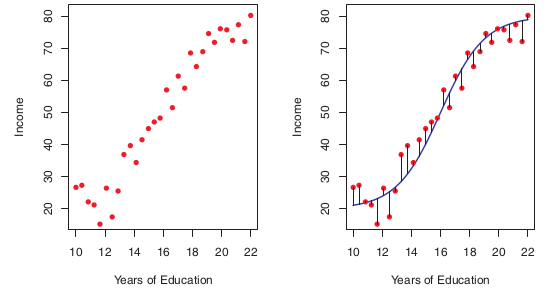
\includegraphics[width=.5\textwidth]{./chap/1chap/1sec/1images/1_1estimationOfF.png}
  \caption{Estimation of $f$}
  \label{fig:1.1}
\end{figure}\\
\begin{figure}[H]
  \centering
  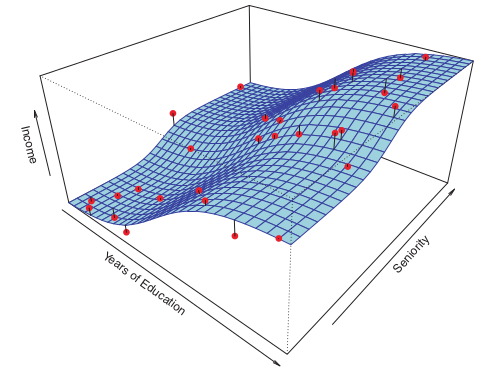
\includegraphics[width=.5\textwidth]{./chap/1chap/1sec/1images/1_2estimationF2D.png}
  \caption{Estimation of $f$ in $2-D$}
  \label{fig:1.1}
\end{figure}
In essence \textbf{Statistical Learning} refers to a set of approaches
for estimating $f$.
\paragraph{Why estimate $f$}
\subparagraph{Prediction}
\encV{$\widehat{Y}=\widehat{f}\left( X \right)$}
$
\begin{cases}
  \widehat{f}\text{ represents our estimating for }f\\
  \widehat{Y}\text{ represents the resulting prediction for }Y
\end{cases}$\\
$\widehat{f}$ is often treated as a \emph{black box} since \tB{we pay
more attention to its prediction accuracy than its exact form}.\\
The accuracy of $\widehat{Y}$ depends on $2$ quantities\\
$\begin{cases} 
  reductible~error\text{, can be \tB{improved by using most appropriate
  statistical learning technique}}\\
  irreductible~error\text{, cannot be changed and \tB{have external 
  causes which are out of control}}
\end{cases}$\\
 simple calculus shows that:
\begin{align*}
  \E{\left[Y-\widehat{Y}\right]^{2}}&=\E{\left[f\left( X \right)+\epsilon-\widehat{f}\left( X \right)\right]^{2}}\\
  &= \underbrace{\E{\left[ f\left( X \right)-\widehat{f}\left( X \right) \right]^{2}}}_{Reducible}+\underbrace{\V{\epsilon}}_{Irreducible}\text{ think that $\E{\epsilon}=0$}
\end{align*}
\subparagraph{Inference} Now we want to know how $Y$ evolves when $X$
changes, so we cannot considerate anymore $f$ as a black box.\\
\begin{itemize}
\item \emph{Which predictors are associated with the response?} (\tB{to
discover variables which have the most important influence therewith 
to reduce number of considered variables})
\item \emph{What is the relationship between the response and each
  predictor?}(\tB{Which components increase Y value and which decrease
  it})
\item \emph{\tB{Can the relationship between $Y$ and each predictor be
	adequately summarized using linear equation} or is the relationship
more complicated?}
\end{itemize}
\paragraph{How do we estimate $f$}
\subparagraph{Aim} Let $(i,j)\in\inter{1}{n}\times\inter{1}{p}$ and 
\tB{$x_{ij}$ represent the value of the $j^{th}$ predictor for $i^{th}$
observation}. Correspondingly let $y_{i}$ represent the response 
variable for the $i^{th}$ observation.\\
Then our training data consists of $\left\{ \left( x_{i},y_{i}
\right)_{1\leq i\leq n}\right\}\text{ where }x_{i}=\begin{pmatrix}
x_{i1}\\.\\.\\.\\x_{ip}\end{pmatrix}$.\\
\tR{We want to find a function $\widehat{f}$ such that $Y\approx
\widehat{f}\left( X \right)$ for any observation $\left( X,Y \right)$}
\subparagraph{Parametric methods}
\begin{enumerate}
	\item \tB{\emph{Assumption about functional form of $f$}}\\ For
		example: $f\left( X \right)=\beta_{0}+\su{{i=1}}{p}
		\beta_{i}X_{i}$ in this case instead to estimate 
		entirely $p$-dimensional function $f$ we only need to
		estimate $\left( \beta_{i} \right)_{0\leq i\leq p}$
  \item After the model selection, \tB{we need a procedure which uses
\emph{data training} to \textit{fit} or \textit{train} the model}.
    \\For example we need to estimate
    $\left( \beta_{i} \right)_{0\leq i\leq p}$ such that:
    $Y\approx\beta_{0}+\su{{i=1}}{p}\beta_{i}X_{i}$\\ The most common
    approach to fit the model is \emph{least squares}.
\end{enumerate}\encV{
The parametric methods allow to reduce the problem of estimating $f$
down
to one of estimating a set of parameters}.
\begin{figure}[H]
\begin{subfigure}{0.5\textwidth}
  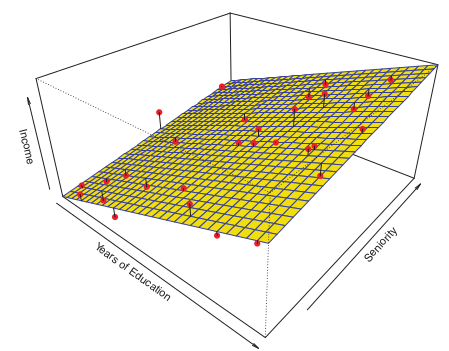
\includegraphics[width=0.9\linewidth, height=5cm]{./chap/1chap/1sec/1images/1_3linearEstimation.png} 
  \caption{Linear estimation:\\$income=\\\beta_{0}+\beta_{1}\times education+\beta_{2}\times seniority$}
  \label{fig:1.3_1}
\end{subfigure}
\begin{subfigure}{0.5\textwidth}
  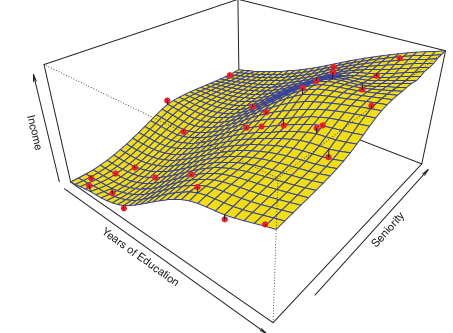
\includegraphics[width=0.9\linewidth, height=5cm]{./chap/1chap/1sec/1images/1_4BestEstimation.png} 
  \caption{Best estimation of $f$ for\\ $income\approx f\left( income,seniority \right)$}
  \label{fig:1.3_2}
\end{subfigure}
\caption{Estimation of $f$ with 2 degrees of precision}
\label{fig:1.4}
\end{figure}

\subparagraph{Non-Parametric methods}
Any parametric approaches brings with it the possibility that the
functional form used to estimate $f$ is very different from the true
$f$. In contrast non-parametric approaches completely avoid this danger
since \tB{no assumption about the form of $f$ is made.} But non
parametric approaches do suffer from non-reducing problem, and \sB{they
need a very greater number of observation than with parametric 
approaches}.
\paragraph{The trade-off between Prediction Accuracy and model
Interpretability}
When inference is the goal, there are clear advantages to using simple
and relatively inflexible statistical learning methods.
\begin{figure}[H]
   \centering
   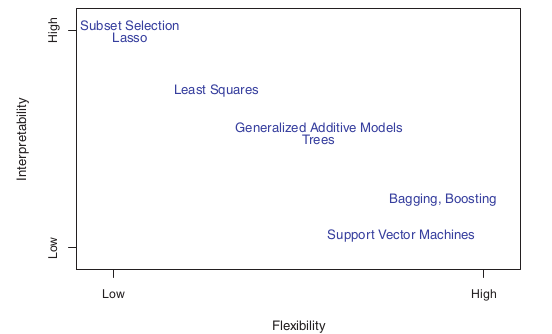
\includegraphics[width=.7\textwidth]{./chap/1chap/1sec/1images/1_5ToChooseAgoodApproach.png}
   \caption{To know which methods to use.}
   \label{fig:1.4}
 \end{figure}
 \paragraph{Supervised versus unsupervised learning}
 We speak about \tR{\emph{supervised problems}} \sR{when for each predictors
 $x_{i}$ there is an associated response measurement $y_{i}$}.\\
 Whereas in \tR{\emph{unsupervised problems}} \sR{we observe a vector of
 measurements $x_{i}$ but not associated response $y_{i}$}. Then we can
 seek to understand the relationship between the variables or between
 observations.\\ One statistical tool that we may use in this setting
 is \emph{clustering}
 \begin{figure}[H]
   \centering
   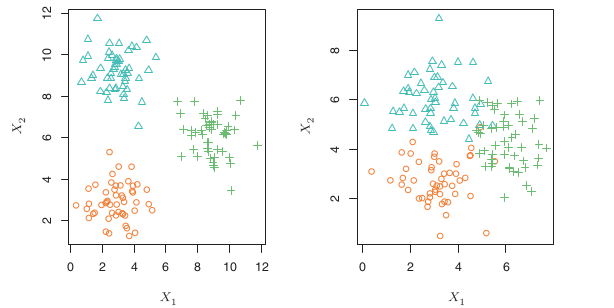
\includegraphics[width=.7\textwidth]{./chap/1chap/1sec/1images/1_6Clustering.png}
   \caption{Clustering methods is used for \emph{unsupervised problems}.}
   \label{fig:1.5}
 \end{figure}
 \paragraph{Regression versus Classification problems}
 In general Regression is used for quantitative variables whereas
 classification is used for qualitative variables but we can find
 several counter-examples.

\subsection{Assessing Model Accuracy}
\paragraph{Measuring the quality of a fit}
In regression setting, the most commonly-used measure of model accuracy
is the \tR{\emph{Mean Squared Error (MSE)}}:\encV{$MSE=\dfrac{1}{n}
\su{{i=1}}{n}\left( y_{i}-\widehat{f}\left( x_{i} \right) \right)^{2}$}
\\We do not really care about whether for all $i\in\inter{1}{n}
\widehat{f}\left( x_{i} \right)\approx y_{i}$, instead \tB{we want to 
know whether a previously unseen observation not used to train the
statistical learning method $\left( x_{0},y_{0} \right)$ is such that
$\widehat{f}\left( x_{0} \right)\approx y_{0}$}.\\In other words if we
had a large number of test observations, we could compute \encV{$Ave
\left( \left(y_{0}-\widehat{f}\left( x_{0} \right)\right)^{2} \right)$}
\tR{We want to choose the method that gives the lowest \emph{test MSE},
as opposed to the lowest \emph{training MSE}}.\\Many 
statistical methods estimate coefficients so as to minimize the 
training set MSE, then training set MSE can be quite small, but test
MSE is often much larger.
\begin{figure}[H]
  \centering
  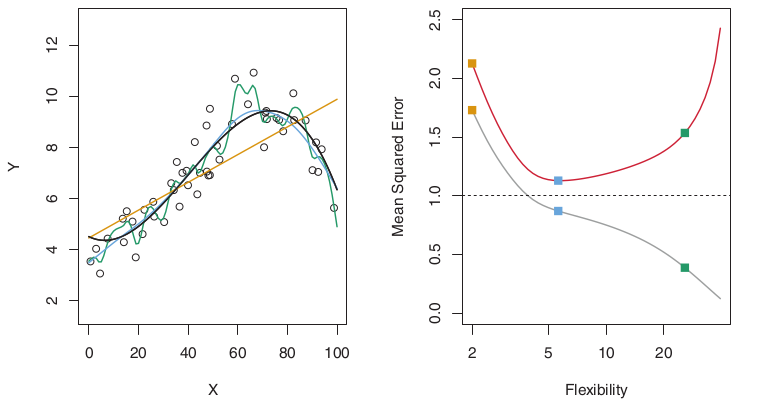
\includegraphics[width=\textwidth]{./chap/1chap/1sec/2images/2_1trainingMSEandTestMSE.png}
  \caption{Left:Data simulated from $f$, shown in black and 3 estimates
  of $f$\\Right: Training MSE in grey and test MSE in red.\\Squares
represent the training and test MSEs for the 3 fits shown in the 
left-hand pannel}
  \label{fig:2.1}
\end{figure}
The blue curve minimizes the test MSE, and visually appears to estimate
$f$ the best in the left-hand panel.\\\tR{The horizontal dashed line
indicates $\V{\epsilon}$ the irreducible error in which corresponds
to the lowest achievable test MSE among all possible methods.}\\
\tB{When a given method yields a high training MSE but a low test MSE 
we say that data are \emph{overfitting}}.

\paragraph{The Bias-Variance Trade-Off}\enc{
$\E{\left( y_{0}-\widehat{f}\left( x_{0} \right) \right)^{2}}=
\V{\widehat{f}\left( x_{0} \right)}+\left[ Bias\left( \widehat{f}
\left( x_{0} \right)\right) \right]^{2}+\V{\epsilon}$}
$\begin{cases}\E{\left(y_{0}-\widehat{f}\left(x_{0}\right)\right)^{2}}
\text{ defines the \tB{\emph{expected test MSE}} and refers to the 
average test MSE.}\\\V{\hat{f}(x_{0})}\text{ the amount by which $\widehat{f}$ 
would change if we estimating it using a different training data.}\\
\left[Bias\left(\hat{f}(x_{0})\right)\right]^{2}\text{ refers to the error that is introduced by approximating a
real-life problem.}\end{cases}$\\As we increase the flexibility of a
class methods, the bias tends to initially decrease faster than the 
variance increases. 
\begin{figure}[H]
  \centering
  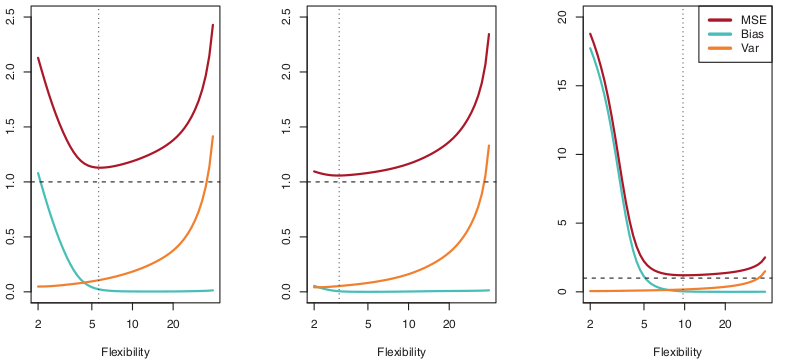
\includegraphics[width=\textwidth]{./chap/1chap/1sec/2images/2_2biaisVarianceMSE.png}
  \caption{Squared bias, variance and test MSE.\\$\V{\epsilon}$ indicates by the dashed line.}
  \label{fig:2.1}
\end{figure}
\subsection{Bias, Variance and Model Complexity}
The Loss function for measuring errors between $Y$ and $\hat{f}(X)$ is denoted by $L\left(Y,
\hat{f}(X)\right)$. Typical choices are: 
$$ L\left(Y,\hat{f}(X)\right) = 
\begin{cases}
	\left(Y-\hat{f}(X)\right)^{2}\text{ squared error}\\
	\left|Y-\hat{f(X)}\right|\text{ absolute error}
\end{cases}
$$
There are 3 important quantities:
$$ 
\begin{cases}
	\overline{err} = \dfrac{1}{N}\su{{i=1}}{N}L\left(y_{i},\hat{f}(x_{i})\right)\\
	Err_{\mathcal{T}}=\E{L\left(Y,\hat{f}(X)\right)|\mathcal{T}}\text{ \emph{Test error}}\\
	Err=\E{L\left(Y,\hat{f}(X)\right)}=\E{Err_{\mathcal{T}}}\text{ \emph{Test error}}
\end{cases}
$$
\paragraph{The classification setting}
Suppose that we seek to estimate $f$ on the basis of training 
observations $\left\{ \left( x_{i},y_{i} \right) \right\}_{1\leq i\leq
n}$ where now $\left( y_{i} \right)_{1\leq i\leq n}$ are qualitative.\\
The most common approach for quantifying the accuracy of our estimate
$\widehat{f}$ is the \tB{training \emph{error rate}}:\\
\enc{$\dfrac{1}{n}
\su{{i=1}}{n}I_{y_{i}\neq \widehat{y}_{i}}\text{ with }I_{y_{i}\neq
\widehat{y}_{i}}\begin{cases}1\Leftarrow y_{i}\neq \widehat{y}_{i}\\0
\Leftarrow y_{i}=\widehat{y}_{i}\end{cases}$}.\\ The \emph{test error
rate} associated with a set of test observation of the form $\left( 
x_{0},y_{0} \right)$ is given by:\encV{$Ave\left( I_{y_{0}\neq 
\widehat{y}_{0}} \right)$}
%\subparagraph{The Bayes Classifier}
%\sB{The test error rate is minimized, on average, by a very simply 
%classifier that assigns each observation to the most likely class}. We
%should simply assign a test observation with predictor vector $x_{0}$
%to the class $j$ for which $\ProbC{X=x_{0}}{Y=j}$ is largest.
%\begin{figure}[H]
%  \centering
%  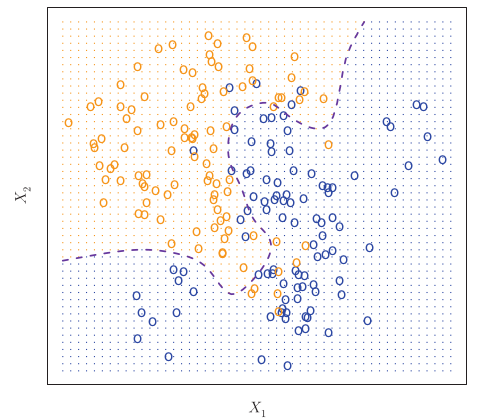
\includegraphics[width=\textwidth]{./chap/1chap/1sec/2images/2_3bayesClassifier.png}
%  \caption{A simulated data set consisting of 100 observations in each
%  of 2 groups, indicated in blue and in orange.\\The purple dashed line
%represents the \emph{Bayes decision boundary}, the orange background
%grid indicates the region in which a test observation will be assigned
%to the orange class, and likewise to blue color.}
%  \label{fig:2.2}
%\end{figure}
%The orange shaded region reflects the set of
%points for which $\ProbC{X}{Y=orange}$ is greater than $50\%$, while 
%the blue shaded region indicates the set of points for which the 
%probability is below $50\%$. The purple dashed line represents the 
%points where the probability is exactly $50\%$. \sB{Since the Bayes 
%classifier will always choose the class for which $\ProbC{X=x_{0}}{Y=j}
%$ is largest, the error rate at $X=x_{0}$ will be $1-\max\limits_{j}
%\ProbC{X=x_{0}}{Y=j}$}.\\ In general, the overall Bayes error rate is
%given by \enc{$1-\E{\max\limits_{j} \ProbC{X}{Y=j}}$}
%\subparagraph{K-Nearest neighbors}
%\sB{For real data we do not know the conditional distribution of $Y$ 
%given $X$ and so computing the Bayes classifier is impossible}.
%Therefore, the Bayes classifier serves as an unattainable gold standard
%against which to compare other methods.\\Given a positive integer $K$ 
%and a test observation $x_{0}$.
%\begin{enumerate}
%  \item It identifies the $K$ points in the training data that are
%    closet to $x_{0}$ represented by $\mathcal{N}_{0}$
%  \item It then estimates the conditional probability for class $j$ as
%    the fraction of points in $\mathcal{N}_{0}$ whose response values
%  equal $j$:$\ProbC{X=x_{0}}{Y=j}=\dfrac{1}{K}\su{{i\in\mathcal{N}_{0}}
%}{{}}I_{y_{i}=j}$
%\end{enumerate}
%\begin{figure}[H]
%  \centering
%  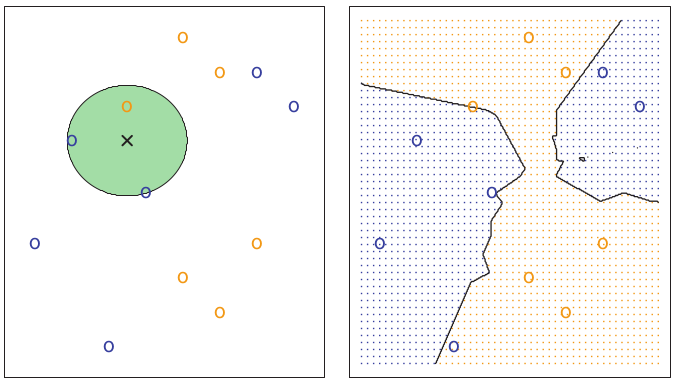
\includegraphics[width=\textwidth]{./chap/1chap/1sec/2images/2_4KNNworking.png}
%  \caption{KNN approach for $k=3$\\A test observation at which a
%  predicted class label is desired is shown as a black cross.\\
%Right-hand panel: The KNN decision boundary for this example is shown
%in black. The blue grid indicates the region in which a test 
%observation will be assigned to the blue class, likewise for the orange
%grid.}
%  \label{fig:2.2}
%\end{figure}Explanation of the KNN approach:\\
%Suppose that we choose $K=3$, then KNN will first identify the 3
%observations that are closet to the cross. This neighborhood is shown
%as a circle. It consists of 2 blue points and 1 orange point, resulting
%in estimated probabilities of $\frac{2}{3}$ for the blue class and
%$\frac{1}{3}$ for the orange class. Hence KNN will predict that the
%black cross belongs to the blue class.\\\\
%Despite the fact that is a very simple approach, KNN can often produce
%classifiers that are surprisingly close to the optimal Bayes classifier.
%\begin{figure}[H]
%  \centering
%  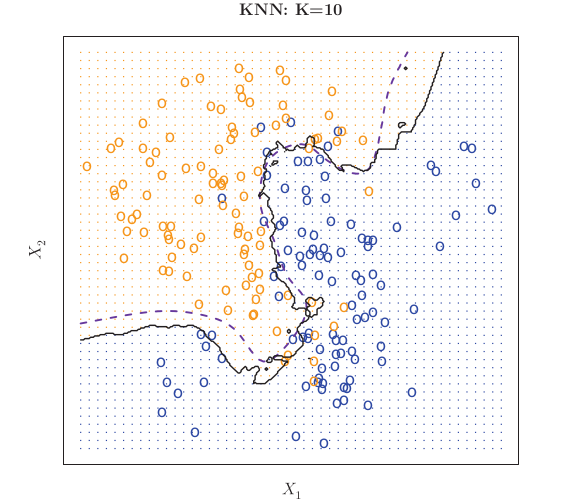
\includegraphics[width=\textwidth]{./chap/1chap/1sec/2images/2_5KNNboundary.png}
%  \caption{The black curve indicates the KNN decision boundary with
%  K=10.\\The Bayes decision boundary is shown as a purple dashed line.}
%  \label{fig:2.2}
%\end{figure}
%As $K$ grows, the method become less flexible and produces a decision
%boundary that is close to linear. This corresponds to a low-variance,
%but high-bias classifier

%\subsection{Introduction to R}
%\begin{itemize}
	\item
 \end{itemize}

%%\subsection{Exercises}
%%\paragraph{Conceptual}
\begin{enumerate}
 \item
   \begin{itemize}
     \item[(a)] The number of predictors being small, and sample size
being extremely high, and knowing the expected test MSE $\E{\left( 
y_{0}-\widehat{f}\left( x_{0} \right) \right)^{2}}=\V{\widehat{f}\left(
x_{0} \right)}+\left[ Biais\left( \widehat{f}\left( x_{0} \right)
\right) \right]^{2}+\V{\epsilon}$ which refers to the average test MSE.
\\A great number of observations results an increase of the variance.
Then to compensate this increasing we should use a unflexible method,
because unflexible methods decrease the variance.\\Then we avoid the
overfitting risk.
\item[(b)] It is the opposite case, now the low amount number of
observations results to a high probability to make mistakes on our
approximate function $f$. This means that biais increases, therefore
we should use a flexible methods therewith to componsate the biais
increasing. However the variance will increase but it's not a problem
because the number of observation is small.
\item[(c)] If the relationship between predictors and response is
highly non-linear we need a method with a high level of flexibility.
Then the challange is to approximate the real life problem therefore we
must reduce the biais.
\item[(d)] We have no control on the $\epsilon$ so I do not know.
   \end{itemize}
 \item
   \begin{itemize}
     \item[(a)] Our predictors are almost all quantitative, there is
just the industry predictor which is qualitative however we can assign
a number in function of the industry.\\Then it looks like a regression
problem. We are most interested in inference.$n=500,p=4$
\item[(b)] Our predictors are all quantitative but response is
qualitative.\\Then it looks like a classification problem. We are most
interested in prediction $n=20,p=14$
\item[(b)] Our predictors are all quantitative and the response 
searched is quantitative.\\Then it looks like a
regression problem. We are most interested in prediction $n=?,p=4$
   \end{itemize}
 \end{enumerate}


\section{Linear Regression}
\begin{itemize}
	\item
 \end{itemize}
\subsection{Simple linear regression}
In general simple linear regression is written as:\encV{$Y\approx
\beta_{0}+\beta_{1}X$}.\\We might read ``$\approx$'' as ``is 
approximately modeled as''

\paragraph{Estimating the Coefficients}
Let $\left\{ \left( x_{i},y_{i} \right) \right\}_{1\leq i\leq n}$
represent $n$ observations, our goal is to obtain coefficient estimates
$\widehat{\beta}_{0},\widehat{\beta}_{1}$ such that the linear model
fits the available data well, so that $y_{i}\approx\beta_{0}+\beta_{1}
x_{i}$ for $i\in\inter{1}{n}$, in other words we want an \emph{
intercept} $\beta_{0}$ and a \emph{slope} $\beta_{1}$\\For $i\in\inter{1
}{n}, e_{i}=y_{i}-\widehat{y}_{i}$ represents the $i^{th}$ \emph{
residual}\\
Then we define the \begin{center}\enc{$\text{RSS(\tR{Residual Sum of
Squares})}=\su{{i=1}}{n}e_{i}^{2}=\su{{i=1}}{n}\left( y_{i}- \widehat{
\beta_{0}}-\widehat{\beta_{1}}x_{i}\right)^{2}$}\end{center}.Using some calculus show 
that minimizers are \enc{$\begin{cases}\widehat{\beta_{1}}=\dfrac{\su{{
i=1}}{n}(x_{i}-\overline{x})(y_{i}-\overline{y})}{\su{{i=1}}{n}(x_{i}-
\overline{x})^{2}}\\\widehat{\beta}_{0}=\overline{y}-\widehat{\beta}_{1
}\overline{x}\end{cases}$}
\begin{figure}[H]
  \centering
  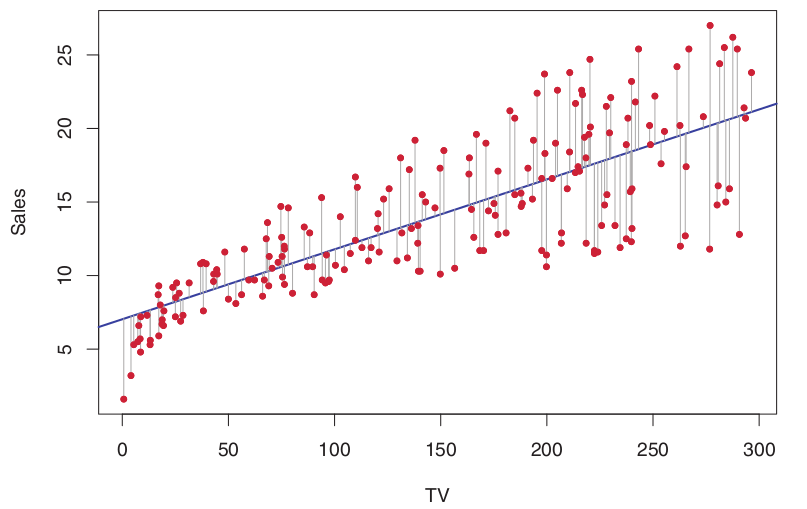
\includegraphics[width=.3\textwidth]{./chap/1chap/2sec/1images/1_leastSquares.png}
  \caption{The least squares fit for the regression of sales onto TV.}
  \label{fig:2.1}
\end{figure}
We can see on the following plots, that $\widehat{\beta}_{0},\widehat{\beta}_{1}$ minimize the RSS.
\begin{figure}[H]
  \centering
  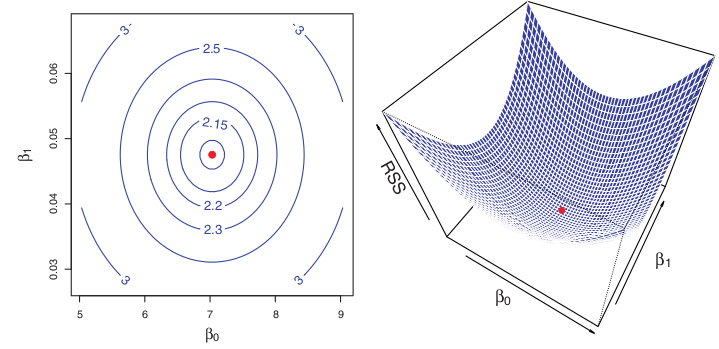
\includegraphics[width=.5\textwidth]{./chap/1chap/2sec/1images/2_leastSquaresCoefficients.png}
  \caption{Contour and 3-dimensionnal plots of the RSS on the 
Advertising data, using sales as the response and TV as the predictor}
  \label{fig:2.2}
\end{figure}

\paragraph{Assessing the Accuracy of the Coefficient Estimates}
When we assume that there is a relation between $X\text{ and }Y$ then
$Y=f\left( X \right)+\epsilon\begin{cases}f\text{ is a uknown function
 }\\\epsilon\text{ is a mean-zero random error term, is a catch-all for
what we miss with this simple model}\end{cases}$\\If $f$ is to be 
approximated by a linear function then we can write this relationship
as \encN{$Y=\beta_{0}+\beta_{1}X+\epsilon$}.\\This equation defines the
\emph{population regression line} which is the best approximation to
the true relationship between $X$ and $Y$.\\ We created $100$ random
$X_{s}$ and generated $100$ corresponding $Y_{s}$ from the model $Y=2+
3X+\epsilon$ where $\epsilon$ is generated from a normal distribution
with mean zero.
\begin{figure}[H]
  \centering
  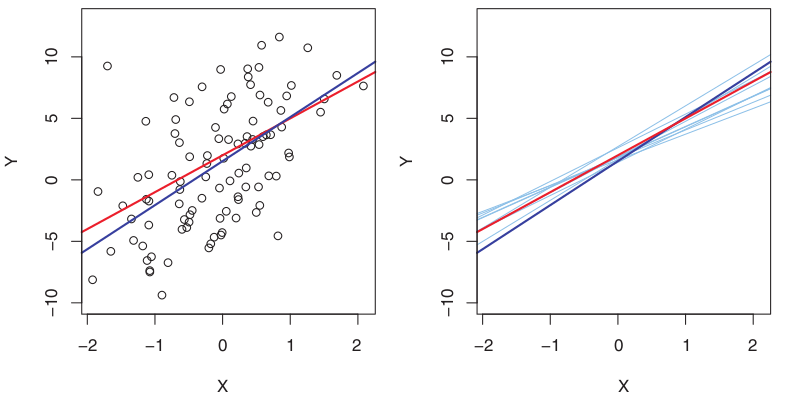
\includegraphics[width=\textwidth]{./chap/1chap/2sec/1images/3_leastSquaredErrorLineVsPopulationRegressionLine.png}
  \caption{The left-hand pannel:red line is the popuation regression
  line, and in blue line the least squares estimate for $f(X)$ bassed
  on the observed data, shown in black.\\The right-hand pannel: is the
  same graph that left-hand pannel but with 10 other least sqaures
  estimates with each a distinct training data set but from the same
  model}
  \label{fig:2.3}
\end{figure}
If we use the sample mean $
\widehat{\mu}$ to estimate $\mu$ this estimate is \emph{unbiased}, in
the sense that on average, we expect $\widehat{\mu}$ to equal $\mu$\\
We have etablished that the average $\widehat{\mu}$'s over many data
sets will be very close to $\mu$ but that a single estimate $\widehat{
\mu}$ may be a substantial underestimate or overestimate of $\mu$.
\tB{How far off will that single estimate of $\mu$ be? We generally 
answer to this question by computing the \emph{SE (Standard Error)} of
$\widehat{\mu}$ written as $SE(\widehat{\mu})$}:\begin{center}\enc{
$\V{\widehat{\mu}}=SE\left( \widehat{\mu} \right)^{2}=\dfrac{\sigma^{2}
}{n}$}\\$\sigma$ is the standard deviation of each of the realizations 
$y_{i}$ of $Y$.\end{center}
\begin{center}\enc{$
\begin{cases}SE\left(\widehat{\beta}_{0}\right)^{2}=\sigma^{2}\left[
\dfrac{1}{n}+\dfrac{\overline{x}^{2}}{\su{{i=1}}{n}\left(x_{i}-
\overline{x}\right)^{2}}\right]\\
SE\left(\widehat{\beta}_{1}\right)^{2}=
\dfrac{\sigma^{2}}{\su{{i=1}}{n}\left(x_{i}-\overline{x}
\right)^{2}}\end{cases}$}\\$\sigma^{2}=\V{\epsilon}$\end{center}\Moi{$SE\left(\widehat{\beta_{1}}
\right)$ is smaller when the $x_{i}$ are more spread out}For these
formulas we need to assume that the errors $\epsilon_{i}$ are
uncorrelated with $\sigma^{2}$. This is cleary not true but the formula
still turn out to be a good approximation.\\\sB{In general $\sigma$ is
unknown but can be estimated from the data, the estimate of $\sigma$ is
known as} \tR{\emph{Residual Standard Error}} \encB{$RSE=\sqrt{\dfrac{
RSS}{n-2}}$}.\\\Moi{Roughly speaking when $\sigma^{2}$ is estimated we
should write $\widehat{SE\left(\widehat{\beta_{1}}\right)}$}\\\\
Standard can be used to define \emph{confident interval}
\tR{For linear regression the $95\%$ confident intervals are} \begin{center}
\enc{$\begin{cases}\widehat{\beta_{0}}\pm 2\times SE\left(\widehat{
\beta_{0}}\right)\\\widehat{\beta_{1}}\pm 2\times SE\left(\widehat{
\beta_{1}}\right)\end{cases}$}\end{center}Standard error can be used
to perform hypothesis test, the most common test involves \emph{null
hypothesis} and \emph{alternative hypothesis}:\encB{$\begin{cases}
H_{0}:\beta_{1}=0\\H_{\alpha}:\beta_{1}\neq 0\end{cases}$}\\To test
null hypothesis we need to determine wehter $\widehat{\beta_{1}}$ is
sufficiently
far from zero that we can be confident that $\beta_{1}$ is non-null.\\
\emph{How far is far enough?} This depends on the $\widehat{\beta_{1}}$
accuracy then \\$\begin{cases}SE\left(\widehat{\beta_{1}}\right)\text{
is small, even relatively small values of }\widehat{\beta_{1}}\text{
can be a strong evidence that }\beta_{1}\neq 0\\SE\left(\widehat{
\beta_{1}}\right)\text{ is large then }\widehat{\beta_{1}}\text{ must 
be large in absolute value in order for us to reject }H_{0}\end{cases}$
\\In practice we compute a \emph{t-statistic} given by \begin{center}
\enc{$t=\dfrac{\widehat{\beta_{1}}-0}{SE\left(\widehat{\beta_{1}}
\right)}$}\\which measure the number of standard deviation that $
\widehat{\beta_{1}}$ is away from $0$.\end{center} \tB{If there is no
relationship between $X$ and $Y$ then we except that we will have a 
\emph{ t-distribution}}. It is a simple matter \tR{to observe the 
probability of observing any number equal to $|t|$ or larger in
absolute
value, \emph{assuming that }$\beta_{1}=0$} this probability is called
\tR{\emph{p-value}}.\\Roughly speaking a small \emph{p-value} indicates
that it is unlikely to observe such a substantial association between
the predictors and the response due to chance.\\\encN{Typical \emph{
p-value} cutoffs for rejecting $H_{0}$ is $5-1\%$}
\paragraph{Assessing the accuracy of the model}
Once we have rejected the null hypothesis in favor of the alternative
hypothesis it is natural to want to qualify to which the model fits the
data.
\subparagraph{Residual Standard Error} \tB{is an estimate of standard
deviation of $\epsilon$}, it means the average amount that the response
will deviate from the true regression line.
\subparagraph{$R^{2}$ statistic} it provides an alternative measure of
fit, and takes the form of a \emph{proportion} (the proportion of
variance explained). \tB{\emph{Total Sum of Squares}} \enc{$TSS=\su{{i=1}}{n
} \left(y_{i}-\overline{y}\right)^{2}$} represents the amount of 
variability
inherent to the response before the regression is performed, in 
contrast \emph{RSS measures the amount of variability that left
unexplained after performing regression}. \begin{center}\enc{$R^{2}=
	\dfrac{TSS-RSS}{TSS}$}\\Then $R^{2}$ measures the \emph{proportion of
variability in $Y$ that can be explained using $X$}\end{center}Recall
that \tR{correlation} defined as \begin{center}\enc{$\widehat{Cor(X,Y)}=
\dfrac{\su{ {i=1}}{n}\left(x_{i}-\overline{x}\right)\left(y_{i}-
\overline{y}\right)}{\sqrt{\su{ {i=1}}{n}\left(x_{i}-\overline{x}
\right)^{2}}\sqrt{\su{ {i=1}}{n}\left(y_{i}-\overline{y}\right)^{2}}}
$}\\$r=\widehat{Cor\left(X,Y\right)}$ is also a measure of the linear
relationship between $X$ and $Y$\end{center}\Moi{it can be shown that
in the simple regression setting $R^{2}=r^{2}$}

\subsection{Multiple linear regression}
\paragraph{Estimating the Regression Coefficients}
A common way to estimate the parameters of a statistical model is to compute
the MLE(Maximum Likelihood Estimation) defined as 
$$\hat{\bm{\theta}} \triangleq \displaystyle \argmax_{\theta} \log\left(
p(\mathcal{D}|\bm{\theta})\right)$$
\begin{align*}
    l(\bm{\theta}) &\triangleq \log\left(p(\mathcal{D}|\bm{\theta})\right)\\
                   &=\su{i=1}{n}\log\left(p(y_{i}|\bm{x_{i}}, \bm{\theta})\right)\\
                   &= \su{i=1}{n}\log\left(
                       \left[\dfrac{1}{2\pi\sigma^{2}}\right]^{\frac{1}{2}}
                       \exp\left(-\dfrac{1}{2\sigma^{2}}\left[y_{i} - \bm{\beta}^{T}
                       \bm{x_{i}}]\right]^{2}\right)\right)\\ 
                   &= \dfrac{1}{2\sigma^{2}}RSS(\bm{\beta}) +
                   \dfrac{n}{2}\log(2\pi\sigma^{2})
\end{align*}
Then the Residual Sum of Squares (RSS) is equal to $\su{i=1}{n}\left(
y_{i}-\beta^{T}x_{i}\right)^{2}$
Instead of maximizing the log-likelihood we can equivalently minimize the Negative Log Likelihood (NLL) 
\begin{center}
    $NLL(\beta) \triangleq l(\beta)$
\end{center}


Considering $\bm{X}$ the $N\times (p+1)$ matrix with each row an input
vector and $y$ be the $N-vector$ of outputs in the training set.
\begin{center}
	$RSS(\beta)=(y-\bm{X}\beta)^{T}(y-\bm{X}\beta)$
\end{center}
Differentiating with respect to $\beta$ we obtain:
$
\begin{cases}
	\dfrac{\partial RSS}{\partial\beta}=-2\bm{X}^{T}(y-\bm{X}\beta)\\
	\dfrac{\partial^{2} RSS}{\partial\beta\partial\beta^{T}}=2\bm{X}^{T}\bm{X}\\
\end{cases}
$\\
Assuming that $\bm{X}$ has full column rank, we set the first 
derivative to 0:\\ $\bm{X}^{T}(y-\bm{X}\beta)=0$ to obtain the unique
solution:

\begin{center}
	\encB{$\hat{\beta}=(\bm{X}^{T}\bm{X})^{-1}\bm{X}^{T}\bm{y}$}
\end{center}
\begin{figure}[H]
\centering
\begin{subfigure}{.5\textwidth}
  \centering
	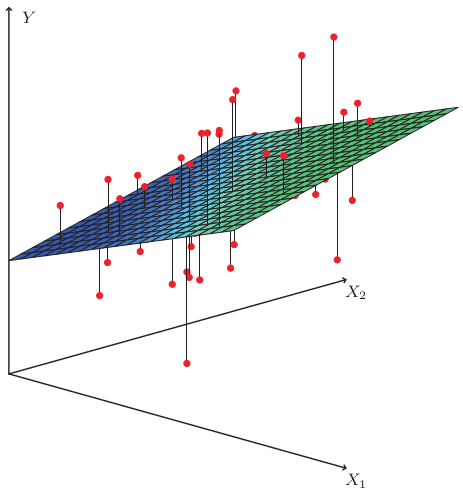
\includegraphics[width=.7\textwidth]{./chap/1chap/2sec/2images/1leastSquaresPlan.png}
  \caption{$n$ observations}
  \label{fig:2.1aLeastSquares}
\end{subfigure}%
\begin{subfigure}{.5\textwidth}
  \centering
	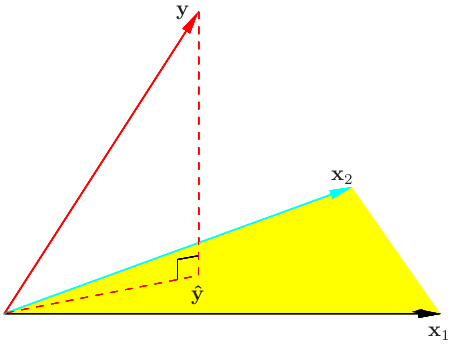
\includegraphics[width=\textwidth]{./chap/1chap/2sec/2images/11projection.png}
\caption{1 observation}
  \label{fig: 2.1bLeastSquares}
\end{subfigure}
  \caption{Least squares for a linear model with $2$ predictors of 
$p$-dimensions.}
\label{fig:test}
\end{figure}

\begin{align*}
\hat{\bm{y}} &=\bm{X}\hat{\beta}\\
	     &=\bm{X}\left(\bm{X}^{T}\bm{X}\right)^{-1}\bm{X}^{T}\bm{y}\\
	     &=\bm{H}\bm{y}
\end{align*}
$\bm{H}$ is called \tB{``hat'' matrix because it puts the hat on $\bm{y}$}.
\paragraph{Hat Matrix}
Residuals can also be expressed as a function of $\bm{H}$,
$\bm{\hat{e}} = \bm{y} - \bm{\hat{y}} = \bm{y} - \bm{Hy} = (\bm{I}-\bm{H})\bm{y}$.
It can be shown that \sB{$\bm{H}$ and $\bm{I}-\bm{H}$ are orthogonal projections}.\\
One can easily show that \tB{$\bm{H}\bm{H} = \bm{H}$} and $\left(\bm{I-H}\right)\left(\bm{I-H}\right)
= \bm{I-H}$

\subparagraph{Range and Kernel of the Hat Matrix}
$rank(\bm{X}) = rank(\bm{X}^{T}\bm{X}) = p^{*}$
\subparagraph{Residual and Fitted Values}
$\bm{H}(\bm{I}-\bm{H}) = \bm{H} -\bm{HH} = 0$, hence $\sP{\bm{\hat{y}}}{\bm{\hat{e}}} = 0$.
\tB{Therefore $\bm{\hat{y}}$ and $\bm{e}$ are orthogonal} in $\mathbb{R}^{n}$.
\subparagraph{Geometric interpretation}
The degrees of freedom associated with \tB{$\bm{\hat{y}}$ and $\bm{\hat{e}}$ can be seen to simply
be the dimensions of the respective vector subspace in which these 2 vectors have been projected}.\\
The vectors $\bm{y}, \bm{\hat{y}}$ and $\bm{\hat{e}}$ determine 3 points in $\mathbb{R}^{n}$ which
form a right-angled triangle, we can see the decomposition of total sum of squares into estimated
sum of squares and residual sum of squares as a special case of \emph{Pythagoras} theorem.
\subparagraph{Further information}
It might happen that the columns of \sB{$\bm{X}$ are not linearly independent, then
$\bm{X}^{T}\bm{X}$ is singular and the least squares coefficients $\hat{\beta}$ are not uniquely 
defined}.\\ 
Knowing that $\V{\bm{A}\bm{y}}=\bm{A}\V{\bm{y}}\bm{A}^{T}$:
\begin{center}
	\encB{$\V{\hat{\beta}}=\left(\bm{X}^{T}\bm{X}\right)^{-1}\sigma^{2}$}
\end{center}
a estimate of $\sigma^{2}$:$\hat{\sigma}^{2} = \dfrac{1}{N-p-1}\su{{i=1}}{N}(y_{i}-\hat{y}_{i})^{2}$ 
The $n-p-1$ rather than $n$ makes $\hat{\sigma}^{2}$ an unbiased
estimate.\\
$
\begin{cases}
\hat{\beta}\hookrightarrow\mathcal{N}\left(\beta, (\bm{X}^{T}\bm{X})^{-1}\sigma^{2}\right)\\
(n-p-1)\hat{\sigma}^{2}\hookrightarrow\sigma^{2}\chi_{n-p-1}^{2}
\end{cases}
$

\paragraph{Convexity}
Functions having a bowl shape with a unique minimum, more precisely:
$$\forall (\bm{\theta}, \bm{\theta'},\lambda) \in \mathcal{S}\times\mathcal{S}\times[0,1],
~ \lambda\bm{\theta} + (1-\lambda)\bm{\theta'} \in \mathcal{S} \Rightarrow \mathcal{S}
\text{ is \textbf{convex}}$$

\subsection{Other considerations in the regression model}
\begin{itemize}
	\item
 \end{itemize}

\subsection{The marketing plan}
\begin{enumerate}
	\item \emph{Is there a relationship between advertising sales
		and budget?}
		\begin{itemize}
			\item fitting a multiple regression model
			\item $F-statistic$ can be used to determine if
				or not we should reject the null 
				hypothesis, in this case a low 
				$p-value$ corresponding to the 
				$F-statistic$ indicates a clear
				evindence of a relationship.
		\end{itemize}
	\item \emph{How strong is the relationship?}
		\begin{itemize}
			\item RSE
			\item $R^{2}$
		\end{itemize}
	\item \emph{Which media contribute to sales?}
		Examine the $p-values$ associated with each 
		predictor's $t-statistic$
	\item \emph{How large is the effect of each medium on sales?}
		If confidence intervals are narrow and far from $0$ 
		then it provides evindence that exists relationship 
		between predictors.\\The collinearity can cause a wide
		confidence interval, so we could use \emph{VIF} to know
		if there is collinearity.
	\item \emph{How accurately can we predict future sales?}
		\begin{itemize}
			\item To predict an individual response $Y=
				f\left(X\right)+\epsilon$
				we use a \emph{predictor interval}
			\item To predict the average response $f\left(
				X\right)$, we use a confidence interval
		\end{itemize}
	\item \emph{Is the relationship linear?}
		To observe residual plots.
	\item \emph{Is there synergy among the advertising media?}
		In the presence of non-additive relationships we can
		introduce an \emph{interaction term} in the regression.
	\ldots
 \end{enumerate}

\subsection{Comparison of linear regression with K-Nearest neighbors}
\begin{itemize}
	\item
 \end{itemize}

\subsection{Lab: linear regression}
\paragraph{Libraries}
To download package we can do following steps:
\begin{itemize}
 	\item Download targ file on 
	 ``https://cran.r-project.org/web/packages/''
	 \item Compile it with ``sudo R CMD INSTALL''
 \end{itemize}

\subsection{Exercises}
\begin{itemize}
 \item
 \end{itemize}


\section{Classification}
To predict qualitative response is know as \emph{classifying}
%\subsection{An overview of classification}
%\begin{figure}[H]
	\begin{center}
		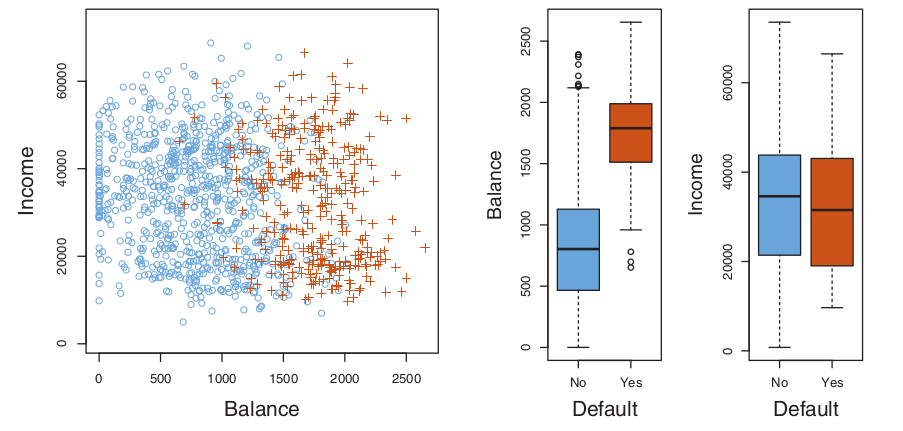
\includegraphics[width=\textwidth]{./chap/1chap/3sec/1images/1DefaultDataSetPlot.png}
	\end{center}
	\caption{The \emph{default} data set.\\Left:indivduals who
defaulted in orange in a given month and those who did not in blue.\\}
Right: The first boxplot shows the balance distribution split by the
binary default variable, the second plot the income distribution.
	\label{fig:fig3.1}
\end{figure}
It appears that individuals who defaulted tended to have a higher 
credit card balances.\\In this chapter we learn how to build a model to
predict default for  any values of balance and income.

\subsection{Why not linear regression ?}
In general there is no natural way to convert a qualitative response 
variable with more than 2 levels into the quantitative response that
is ready for linear regression. 

\subsection{Logistic regression}
\paragraph{The logistic model}
\emph{How should we model the relationship between $\ProbC{X}{Y=1}$ and
$X$?}
\begin{figure}[H]
	\begin{center}
		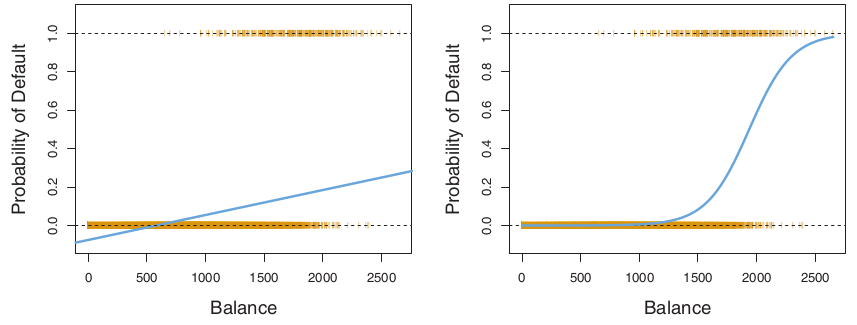
\includegraphics[width=\textwidth]{./chap/1chap/3sec/3images/1ProbabilityOfDefault.png}
	\end{center}
	\caption{Left:Estimated probability of default using linear
regression. Some of estimated probability are negative! The orange 
ticks indicate the $0/1$ values coded for default (NO/YES)\\Right:
Predicted probabilities of default using logistic regression.\\All
probabilities lie between $0$ and $1$.}
	\label{fig:fig3.2}
\end{figure}
\paragraph{The logistic model}
\subparagraph{Assumptions}
\begin{enumerate}
	\item Logistic regerssion must be binary or ordinal.
	\item Mutual independence of observations.
	\item No collinearity
	\item Linearity of qualitative independent variables and log odds.
\end{enumerate}


\subparagraph{Requirement}
\begin{enumerate}
	\item Logistic regression requires quite large sample size.
\end{enumerate}
\subparagraph{Formula}
The logistic regression:
\begin{center}
%	\encN{$p\left(X\right)=\ProbC{X}{Y=1}=\dfrac{e^{\beta_{0}+
%\beta_{1}X}}{1+e^{\beta_{0}+\beta_{1}X}}$}\\
	\encN{$p\left(X\right)=\dfrac{e^{\beta_{0}+
\beta_{1}X}}{1+e^{\beta_{0}+\beta_{1}X}}$}\\
\enc{$\log\left(\dfrac{p\left(X\right)}{1-p\left(X\right)}\right)=
\beta_{0}+\beta_{1}X$}\\ The $\dfrac{p\left(X\right)}{1-p\left(X\right)
}$ quantity is called \emph{odds}.
\end{center}
\paragraph{Estimating the Regression Coefficients}
To fit a logistic model we use the \tR{maximum likelihood} method 
rather that the least squares method (which is a specific case of the
former method). Then we seek estimates $\hb{0}\text{ and }\hb{1}$
such that the predicted probability $\widehat{p}\left(x_{i}\right)$ of
default for each individual corresponds closely as possible to the 
individual default status.
\begin{center}
%	\enc{$\mathcal{L}\left(\hb{0},\hb{1}\right)=\prd{{i:y_{i}=1}}{n}\ProbC{x_{i}}{y_{i}=1}\prd{{j:y_{j}=0}}{n}\left(1-\ProbC{x_{j}}{y_{j}=0}\right)$}\\
\enc{$\mathcal{L}\left(\hb{0},\hb{1}\right)=\prd{i=1}{n}p(x_{i})^{y_{i}}\left(1-p(x_{i})\right)^{1-y_{i}}$}\\
$\hb{0}$ and $\hb{1}$ are chosen to maximize this likelihood function.
\end{center}
%\begin{figure}[H]
%	\begin{center}
%		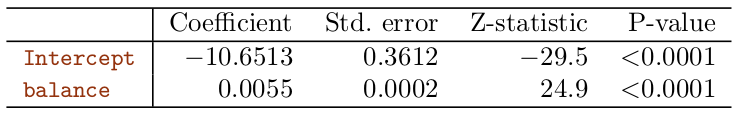
\includegraphics[width=\textwidth]{./chap/1chap/3sec/3images/2estimatesCoeffsLR.png}
%	\end{center}
%	\caption{Estimated coefficients of the logistic regression 
%	model that predict the probability of default using balance.\\
%	A once unit increase in balance is associated with an increase
%	in the log odds of default by $0.0055$ units.}
%	\label{fig:fig3.2}
%\end{figure}
\tB{The \emph{$z$-statistics} plays the same role as \emph{$t$-statistic} in
the linear regression output, $z=\frac{\hb{1}}{SE\left(\hb{1}\right)}$.}
\\The estimated intercept is typically not of interest, its main 
purpose is to adjust the average fitted probabilities to the proportion
of ones in the data.
\paragraph{Marketing Plan}
%\begin{figure}[H]
%	\begin{center}
%		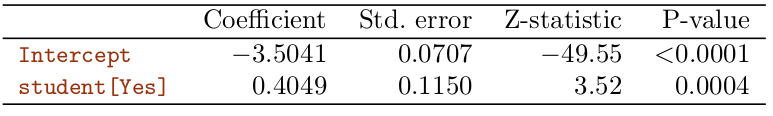
\includegraphics[width=\textwidth]{./chap/1chap/3sec/3images/3LRonDummyVariable.png}
%	\end{center}
%	\caption{Estimated coefficients of the logistic regression
%	model that predicts the probability of default using student
%	status.\\Student status is encoded as a dummy variable, with
%	value 1 for a student and $0$ for a non-student.}
%	\label{fig:fig3.2}
%\end{figure}
$\begin{cases}
	\ProbC{{student=YES}}{\widehat{default}=YES}=\frac{e^{-3.5041+0.4049\times 1}}{1+e^{-3.5041+0.4049\times 1}}=0.0431\\
	\ProbC{{student=NO}}{\widehat{default}=YES}=\frac{e^{-3.5041+0.4049\times 0}}{1+e^{-3.5041+0.4049\times 0}}=0.0292
\end{cases}$\\
This indicates that students tend to have higher default probabilities
than non-student.
\paragraph{Multiple Logistic Regression}
\begin{center}\enc{
$log\left(\dfrac{p\left(X\right)}{1-p\left(X\right)}\right)=\beta_{0}+
\su{{j=1}}{p}\beta_{j}X_{j}$}
\end{center}
%%\begin{figure}[H]
%%	\begin{center}
%%		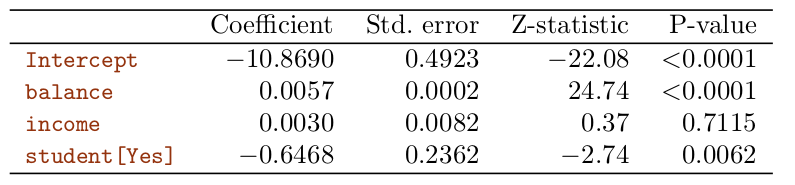
\includegraphics[width=\textwidth]{./chap/1chap/3sec/3images/4multipleLR.png}
%%	\end{center}
%%	\caption{Estimated coefficients of the logistic regression
%%	model that predicts the probability of default using balance,
%%	income and student status.\\Student status is encoded as a
%%	dummy variable, with value 1 for a student and $0$ for a
%%	non-student.\\In fitting this model income was measured in 
%%	thousands dollars.}
%%	\label{fig:fig3.4}
%%\end{figure}
%We surprisingly observe that for given values of income and balance, a
%student is less likely to default than a non-student.
%\begin{figure}[H]
%	\begin{center}
%		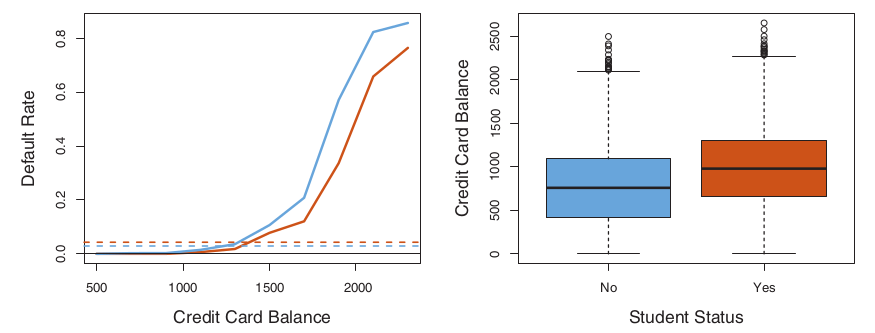
\includegraphics[width=\textwidth]{./chap/1chap/3sec/3images/5confoundingPlot.png}
%	\end{center}
%	\caption{Confounding in the Default data. Left:Default rates
%	are shown for students (orange), and non-students (blue).\\
%	The solid lines show default rate as a function of balance,
%	while horizontal dashed line display the overall default rate
%	\\Right: Boxplots of balance for students and non-students.}
%	\label{fig:fig3.4}
%\end{figure}
%Indeed we observe that from the left-hand panel that the student 
%default rate is at or below of the non-student default rate for every
%value of balance.\\But the horizontal broken lines showing the default
%rate for students and non-students averaged over all values of income
%and balance suggest the opposite effect. Consequently there is a
%positive coefficient for student in the simple logistic regression
%output.\\The right-hand panel provides an explanation for this
%discrepancy, the variables student and balance are correlated. Indeed
%students are more likely to have large credit card balances, which, as
%we know from the left-hand panel tend to be associated to a high 
%default rate. Thus, even though an individual student with a given 
%credit card balance will tend to have a lower probability of default
%than a non-student with the same credit card balance. The fact that 
%students on the whole tend to have a higher credit card balances means
%that overall students tend to default at a higher rate than 
%non-students.
\paragraph{Logistic regression for $p$>2 response classes}
We use \emph{discriminant analysis}
\paragraph{Fitting Logistic Regression Models}
\tB{Logistic regression models are usually fit by maximum of likelihood}, using the conditional 
likelihood of $G$ given $X$. The log-likelihood for $N$ observations is: 
\tB{$$ l(\theta)=\su{{i=1}}{N}log\left( p_{g}(x_{i;\theta}) \right)$$} where $p_{g}(x_{i};\theta)=
\ProbC{X=x_{i}}{G=g;\theta}$.\\
It is convenient to code the two-class $g_{i}$ via a 0/1 response $y_{i}$, where $y_{i}=1$ when
$g_{i}=1$, and $y_{i}=0$ when $g_{2}=2$. Let $p_{1}(x;\theta)=p(x;\theta)$, and 
$p_{2}(x;\theta)=1-p(x;\theta)$. Then the log-likelihood can be written:
\begin{align*}
	l(\beta) =& \su{{i=1}}{N}\left\{ y_{i}\log\left(p(x_{i};\beta)\right)+ (1-y_{i})
	\log\left(1- p(x_{i};\beta)\right)\right\}\\
	=& \su{{i=1}}{N}\left\{ y_{i}\beta^{T}x_{i} - \log\left( 1+e^{\beta^{T}x_{i}} \right) \right\}
\end{align*}

To maximize the log-likelihood, we set its derivatives to zero:
$$ \dfrac{\partial l(\beta)}{\partial\beta} = 
\su{{i=1}}{N}x_{i}\left(y_{i}-p(x_{i};\beta)\right)=0$$ which are $p+1$ equations nonlinear in
$\beta$.
To solve the score, we use the \href{https://en.wikipedia.org/wiki/Newton\%27s_method_in_optimization}{Newton-Raphson} algorithm, which requires the second-derivative or 
Hessian matrix:
$$ \dfrac{\partial^{2}l(\beta)}{\partial\beta\partial\beta^{T}}=\su{{i=1}}{N}
x_{i}x_{i}^{T}p(x_{i};\beta)(1-p(x_{i};\beta))$$
The aim of the Newton-Raphson algorithm is to find the roots of a given real values
function, here $\dfrac{\partial l(\beta)}{\partial\beta}$
Starting with $\beta^{old}$, a single Newton update is : $$ \beta^{new} = \beta^{old} - \left(
\dfrac{\partial^{2}l(\beta)}{\partial\beta\partial\beta^{T}} \right)^{-1}\dfrac{\partial l(\beta)}{
\partial\beta}$$ where the derivatives are evaluated at$\beta^{old}$

Let $\bm{p}$ denote the vector of fitted probabilities with $i^{th}$ element $p(x_{i};\beta^{old})
\text{ and } \bm{W}$ a $N\times N$ diagonal matrix of weights with $i^{th}$ diagonal element
$p(x_{i};\beta^{old})(1-p(x_{i};\beta^{old}))$. Then we have:
\begin{align*}
	\dfrac{\partial l(\beta)}{\partial\beta} =& \bm{X}^{T}(\bm{y}-\bm{p})\\
	\dfrac{\partial^{2} l(\beta)}{\partial\beta\partial\beta^{T}} =&
	-\bm{X}^{T}(\bm{W}-\bm{X})\\
\end{align*}
The Newton step is thus:
\begin{align*}
	\beta^{new} =& \beta^{old} + \left( \bm{X}^{T}\bm{W}\bm{X} \right)^{-1}\bm{X}^{T}(\bm{y}-\bm{p})\\
	=& \left( \bm{X}^{T}\bm{W}\bm{X} \right)^{-1}\bm{X}^{T}\bm{W}\left( \bm{X}\beta^{old}+
	\bm{W}^{-1}(\bm{y}-\bm{p})\right)\\
	=& \left( \bm{X}^{T}\bm{W}\bm{X} \right)^{-1}\bm{X}^{T}\bm{W}\bm{z}
\end{align*}
In the second and third line we have re-expressed the Newton step as a weighted least squares step
with the response: $bm{z} = \bm{X}\beta^{old}+ \bm{W}^{-1}(\bm{y}-\bm{p})$ sometimes known as the
\textbf{adjusted response}.\\
This algorithm is referred to as \textbf{Iteratively Reweighted Least Squares (IRLS)} since each
iteration solves the weighted least squares problem: $$ \beta^{new}\leftarrow\min\limits_{\beta}
\left( \bm{z} - \bm{X}\beta \right)^{T}\bm{W}\left( \bm{z} - \bm{X}\beta \right)$$

It seems that $\beta=0$ is a good starting value for the iterative procedure although convergence
is never guaranteed. Typically the algorithm does converge, since the log-likelihood is concave,
but overshooting can occur.
\tB{Logistic regression models are used mostly as a data analysis and inference tool, where the
goal is to understand the role of the input variables in explaining outcome.}
\emph{Python code}
\begin{python}
import pandas as pd
import sklearn
from sklearn.linear_model import LogisticRegression

y, X = df.iloc[:, 0], df.iloc[:, 1:]
clf = LogisticRegression(random_state=0)
clf.fit(X, y)
print(clf.score(X, y))
\end{python}

\emph{R code}
\begin{rcode}[deletekeywords={model, df, data, family, binomial}]
model.logistic <- glm(y ~ ., data=df, family=binomial)
print(summary(model.logistic))
\end{rcode}
\paragraph{Quadratic Approximations and Inference}
The maximum-likelihood parameter estimates $\hat{\beta}$ satisfy a self-consistency relationship:
they are the coefficients of a weighted least squares fit, where the responses are:
$$ z_{i} = x_{i}^{T}\hat{\beta} + \frac{(y_{i}-\hat{p}_{i})}{\hat{p}_{i}(1_{i}-\hat{p}_{i})}$$

\begin{itemize}
	\item The weighted residual sum-of-squares is the familiar Pearson $\chi^{2}$ statistic:
		$$ \su{{i=1}}{N}\dfrac{(y_{i}-\hat{p}_{i})}{\hat{p}_{i}(1-\hat{p}_{i})}$$ a 
		quadratic approximation of the deviance.
	\item Asymptotic likelihood theory says that if the model is correct, then $\hat{\beta}$
		is consistent.
	\item A central limit theorem then shows that the distribution of $\hat{\beta}
		\hookrightarrow \mathcal{N}\left(\beta,\left(\bm{X}^{T}\bm{W}\bm{X}\right)^{-1} 
		\right)$
	\item Popular shortcuts are the Rao Score test which tests for inclusion of a term, and 
		the Wald test which can be used to test exclusion of a term.
\end{itemize}

\subsection{Linear discriminant analysis}
Why do we need another method that logistic regression in the case of
several response classes?
\begin{itemize}
	\item When classes are well-separated, the \sB{parameter 
		estimates for the logistic regression model are
		unstable}
	\item If \sB{$n$ is small and the distribution of the 
		predictors is approximately normal in each classe}, the
		\emph{linear discriminant model} is \tB{more stable 
		than the logistic.}
	\item Linear discriminant analysis is popular when we have 
		\sB{more than $2$ response classes}.
 \end{itemize}
\paragraph{Using Bayes Theorem for classification}
Let \tB{$\pi_{k}$ represents the prior probability} that a randomly
chosen observation comes from the $k^{th}$ class. Let $f_{k}\text{ such
that }\tB{f_{k}(x) \equiv\ProbC{X=x}{Y=k}}$ the density function of $X$
for an observation that comes from $k^{th}$ class:\\
\enc{$\ProbC{X=x}{Y=k}=\dfrac{\pi_{k}f_{k}(x)}{\su{{j=1}}{K}\pi_{j}f_{j}(x)}$}
\paragraph{Linear Discriminant Analysis for p=1}
Aims:
\begin{enumerate}
	\item \tB{To obtain an estimate for $f_{k}(x)$} that we can plug 
		into\\ $\ProbC{X=x}{Y=k}=\dfrac{\pi_{k}f_{k}(x)}{\su{{j=1}}{K}\pi_{j}f_{j}(x)}$
	\item \tB{To classify an observation to the class for which $p_{k}(x)$} is greatest
\end{enumerate}
Assumption:
$f_{k}(x)$ is \emph{Gaussian} that is $f_{k}(x)=\dfrac{1}{\sqrt{2\pi\sigma_{k}}}e^{-\frac{1}{2\sigma_{k}^{2}}(x-\mu_{k})^{2}}$\\
Knowing that $\sigma_{1}^{2}= \cdots = \sigma_{K}^{2}$ and taking the log of $p_{k}(x)=\dfrac{\pi_{k}\dfrac{1}{\sqrt{2\pi\sigma}}e^{-\frac{1}{2\sigma^{2}}(x-\mu_{k})^{2}}}{\su{{j=1}}{K}\pi_{j}\dfrac{1}{\sqrt{2\pi\sigma}}e^{-\frac{1}{2\sigma^{2}}(x-\mu_{j})^{2}}}$\\
It is equivalent to assigning the observation to the classer for which:
\\
\enc{$\delta_{k}(x)=x\frac{\mu_{k}}{\sigma^{2}}-\frac{\mu_{k}^{2}}{2\sigma^{2}}+ln(\pi_{k})$} is the largest.\\
The \emph{linear discriminant analysis} (LDA) method approximates the
Bayes classifier by plugging estimates for $\pi_{k},\mu_{k}\text{ and }\sigma^{2}$:\\
\encB{
$
\begin{cases}
	\hat{\pi}_{k} = \frac{n_{k}}{n}\\
	\hat{\mu}_{k} = \dfrac{1}{n_{k}}\su{{i:y_{i}=k}}{}x_{i}\\
	\hat{\sigma}^{2} = \dfrac{1}{n-K}\su{{k=1}}{K}\su{{i:y_{i}=k}}{}\left(x_{i}-\hat{\mu}_{k}\right)^{2}
\end{cases}$}

\paragraph{Linear Discriminant Analysis for p>1}
\subparagraph{Assumptions}
\begin{enumerate}
	\item Multivariate normality: independent variables are normal for each level of the grouping
		variable.
	\item Homoscedasticity: variances among group variables are the same accross levels of 
		predictors.
	\item Non-colinearity
	\item Observation are independent 
\end{enumerate}
\subparagraph{Formulas}
Now we assume that $X=\prth{X}{i}{n}\hookrightarrow\mathcal{N}(\mu,\Sigma)$
Here $\E{X}=\mu = 
\begin{pmatrix}
	\mu_{1}\\
	.\\
	.\\
	.\\
	\mu_{p}
\end{pmatrix}
\text{ and } \Sigma = 
\begin{pmatrix}
	Cov\left( X_{1},X_{1} \right) & \cdots & Cov\left( X_{1},X_{j}\right) &\cdots & Cov\left( X_{1},X_{n} \right)\\
	&\cdots& & &\\
	&\cdots& & &\\
	&\cdots& & &\\
	Cov\left( X_{i},X_{1} \right) & \cdots & Cov\left( X_{i},X_{j}\right) &\cdots & Cov\left( X_{i},X_{n} \right)\\
	&\cdots& & &\\
	&\cdots& & &\\
	&\cdots& & &\\
	Cov\left( X_{n},X_{1} \right) & \cdots & Cov\left( X_{n},X_{j}\right) &\cdots & Cov\left( X_{n},X_{n} \right)\\
\end{pmatrix}\\
\text{ and }
\tB{f(x)=\dfrac{1}{(2\pi)^{\frac{p}{2}}|\Sigma|^{\frac{1}{2}}}exp\left( \dfrac{1}{2}(x-\mu)^{T}\Sigma^{-1}(x-\mu) \right)}
	$\\
\text{ then }
$$
\tR{\delta_{k}(x) = x^{T}\Sigma^{-1}\mu_{k}-\dfrac{1}{2}\mu_{k}^{T}\Sigma^{-1}\mu_{k}+ln(\pi_{k})}
$$
\emph{Python code}
\begin{python}
import sklearn
from sklearn.discriminant_analysis import LinearDiscriminantAnalysis

clf = LinearDiscriminantAnalysis()
clf.fit(X, y)
print(clf.score(X, y))
\end{python}

\emph{R code}
\begin{rcode}[deletekeywords={model, lda, data, df}]
library(MASS)

model.lda <- lda(Direction ~ ., data=df)
model.lda
\end{rcode}

\paragraph{Quadratic Discriminant Analysis}
unlike LDA, \tB{QDA assumes that each class has its own covariance matrix}.
That is for an observation from the $k^{th}$ class 
\tR{$X\hookrightarrow N(\mu_{k},\Sigma^{k})$}
\begin{align*}
	\delta_{k}(x) &= -\dfrac{1}{2}(x-\mu_{k})^{T}\Sigma_{k}^{-1}(x-\mu_{k})-\dfrac{1}{2}\ln|\Sigma_{k}|+\ln(\pi_{k})\\
	&= -\dfrac{1}{2}x^{T}\Sigma_{k}^{-1}x+x^{T}\Sigma_{k}^{-1}\mu_{k}-\dfrac{1}{2}\mu_{k}^{T}\Sigma_{k}^{-1}\mu_{k}-\dfrac{1}{2}\ln|\Sigma_{k}|+\ln(\pi_{k})
\end{align*}
\emph{Python code}
\begin{python}
import sklearn
from sklearn.discriminant_analysis import QuadraticDiscriminantAnalysis

clf = QuadrasticDiscriminantAnalysis()
clf.fit(X, y)
print(clf.score(X, y))
\end{python}


\emph{R code}
\begin{rcode}[deletekeywords={model, lda, data, df}]
library(MASS)

model.lda <- lda(y ~ ., data=df)
model.lda
\end{rcode}
\paragraph{Regularized Discriminant Analysis}
The regularize covariance matrices have the form:
\begin{center}
\enc{$ \hat{\bm{\Sigma}}_{k}(\lambda) = \lambda\hat{\bm{\Sigma}}_{k} + (1-\lambda)\hat{\bm{\Sigma}}$}
\end{center}
where $\hat{\bm{\Sigma}}$ is the pooled covariance matrix as used in LDA.
Here \sB{$\lambda\in[0, 1]$ allows a continuum of models between LDA and QDA, $\lambda$ can be 
choosed by cross-validation}.\\
Similar modifications allow $\hat{\bm{\Sigma}}$ itself to be shrunk toward the scalar covariance:
$$ \hat{\bm{\Sigma}}(\gamma) = \gamma\hat{\bm{\Sigma}} + (1-\gamma)\hat{\sigma}^{2}\bm{I}$$
for $\gamma\in [0, 1]$
\emph{R code}
\begin{rcode}
library(klaR)
model.rda <- rda(y ~ ., data=df, gamma=0.05, lambda=0.2)
\end{rcode}
With rda we have :
$\hat{\Sigma}_{k}(\lambda, \gamma)=(1-\gamma)\hat{\Sigma}_{k}(\lambda)+\gamma\dfrac{1}{p}
tr\left(\hat{\Sigma}_{k}(\lambda)\right)I$
\begin{itemize}
	\item[$(\gamma=0,\lambda=0)$]: QDA - individual covariance for each group
	\item[$(\gamma=0,\lambda=1)$]: LDA - a common covariance matrix
	\item[$(\gamma=1,\lambda=0)$]: Conditional independent variables - similar to Naive Bayes,
		but variable variance whithin group (main diagonal elements) are all equal.
	\item[$(\gamma=1,\lambda=1)$]: Classification using euclidian distance - as in previous case,
		but variances are the same for all groups. Objects are assigned to group with nearest
		mean.
\end{itemize}

\paragraph{Computations for LDA}
The \sB{computations of LDA and QDA are simplified by diagonalizing $\hat{\bm{\Sigma}}$ or 
$\hat{\bm{\Sigma}}_{k}$ for the latter}, suppose we compute the eigendecomposistion for each
$\hat{\bm{\Sigma}}_{k} = \bm{U}_{k}\bm{D}_{k}\bm{U}_{k}^{T}\text{ where } \bm{U}_{k}\text{ is }
p\times p$ orthonormal and $\bm{D}_{k}$ a diagonal matrix of positive eigenvalues $d_{kl}$.
\begin{itemize}
	\item $(x-\hat{\mu}_{k})^{T}\hat{\bm{\Sigma}}^{-1}_{k}(x-\hat{\mu}_{k}) =
		\left[ \bm{U}_{k}^{T}(x-\hat{\mu}_{k}) \right]^{T}\bm{D}_{k}^{-1}
		\left[ \bm{U}_{k}^{T}(x-\hat{\mu}_{k}) \right]$
	\item $\log\left( \hat{\bm{\Sigma}}_{k} \right) = \su{l}{}\log(d_{kl})$
\end{itemize}
LDA classifier can be implemented by the following pair of steps:
\begin{itemize}
	\item \sB{\textbf{Sphere} the data with respect to the common covariance estimate $\hat{\bm{\Sigma}}$}:\\ $X^{*} \leftarrow \bm{D}^{\frac{1}{2}}\bm{U}^{T}X$ where $\hat{\bm{\Sigma}} = \bm{U}\bm{D}\bm{U}^{T}$. \sV{The common covariance estimate of $X^{*}$ will now be the identity.}
	\item \tB{Classify to the closet class centroid in the transformed space}, modulo the effect
		of the class prior probabilities $\pi_{k}$.
\end{itemize}

\paragraph{Reduced-Rank Discriminant Analysis}
The $K$ centroids in $p-\text{dimensional}$ input space lie in an affine subspace of dimension
$\leq K-1$, and \sB{if $p$ is much larger than $K$ this will be a considerable drop in dimension}.\\
Moreover in locating the closet centroid \sB{we can ignore distances orthogonal to this subspace, 
since they will contribute equally to each class. Thus we might just as well project the $X^{*}$
onto centroid-spanning subspace $H_{K-1}$} and make distance comparisons there.

Finding the sequences of optimal subspaces for LDA involves the following steps:
\begin{itemize}
	\item compute the \sB{$K\times p$ matrix of class centroids $\bm{M}$} and the common
		\sB{covariance matrix $\bm{W}$}
	\item compute \sB{$\bm{M}^{*} = \bm{M}\bm{W}^{-\frac{1}{2}}$} using the eigen-decomposition 
		of $\bm{W}$
	\item compute \sB{$\bm{B}^{*}$, the covariance matrix of $\bm{M}^{*}$} and its 
		eigen-decomposition \tB{$\bm{B}^{*} = \bm{V}^{*}\bm{D}_{B}(\bm{V}^{*})^{T}$}.
		The columns $v_{l}^{*}$ of $\bm{V}^{*}$ in sequence from first to last \sB{define
		the coordinates of the optimal subspaces}.
\end{itemize}
Combining all these operations \sB{the $l^{th}$ discriminant variable} is given by \tB{$Z_{l}=v_{l}^{
T}X$} with $v_{l}=\bm{W}^{-\frac{1}{2}}v_{l}^{*}$

Fisher arrived at this decomposition via a different route, without referring to Gaussian 
distribution at all.
\begin{center}
	Find the linear combination $Z=a^{T}X$ such that the between class variance is maximized
	relative to the within-class variance.
\end{center}

The \sB{between-class variance of $Z$ is a $a^{T}\bm{B}a$} and the \sB{within-class variance $a^{T}
\bm{W}a$}, where $\bm{W}$ is defined earlier, and $\bm{B}$ is the covariance matrix of the class centroid matrix
$\bm{M}$.\\
Fisher's problem therefore amounts to maximizing the Rayleigh quotient:
\begin{center}
\enc{$ \max\limits_{a}\dfrac{a^{T}\bm{B}a}{a^{T}\bm{W}a}$} 
\end{center}
or equivalently:
$$ \max\limits_{a}a^{T}\bm{B}a \text{ subject to } a^{T}\bm{W}a=1$$
This is a generalized eigenvalue problem, with $a$ given by the largest eigenvalue of $\bm{W}^{-1}
\bm{B}$. 
\begin{itemize}
	\item Gaussian classification with common covariances leads to linear decision boundaries
	\item One can confine the data to the subspace spanned by the centroids in the sphered
		space.
	\item This subspace can be further decomposed into successively optimal subspaces in 
		term of centroid separation. This decomposition is identical to the decomposition
		due to Fisher.
\end{itemize}


\subsection{A comparison of classification methods}
\paragraph{Logistic regression, LDA, QDA and KNN}
\subparagraph{Logistic regression VS LDA}
The only difference between the 2 approaches lies in fact that 
\sB{$\beta_{0}\text{ and }\beta_{1}$ are estimated using maximum 
likelihood, whereas $c_{0}\text{ and }c_{1}$ are computed using the
estimated mean and variance from a normal distribution}.\\
For $p=1~predictor$ we have :
\begin{align*}
	ln\left(\dfrac{p_{1}(x)}{1-p_{1}(x)}\right) &= c_{0} + c_{1}x\text{ LDA}\\
	ln\left(\dfrac{p_{1}(x)}{1-p_{1}(x)}\right) &= \beta_{0} + \beta_{1}x\text{ Logistic regression}\\
\end{align*}
\tB{It is generally felt that logistic regression is a safer, more robust bet than the LDA model,
relying on fewer assumptions.}

\subparagraph{KNN}
KNN is a completely non-parametric approach: no assumptions are made
about the shape of the decision boundary. Therefore, \sB{we can expect this
approach to dominate LDA and Logistic regression when th decision 
boundary is highly non-linear}.

\subparagraph{QDA}
\tB{It is a compromise between the non-parametric KNN method and the 
linear LDA and Logistic regression approaches.}

\subsection{Separating Hyperplanes}
Separating hyperplane classifiers are procedures that construct linear decision boundaries that
explicitly try to separate the data into different classes as well as possible.\\
\sB{Classifier such as $\left\{ x: \hat{\beta}_{0} + \hat{\beta}_{1}x_{1} + \hat{\beta}_{2}x_{2}
= 0 \right\}$ that compute a linear combination of the input features and return the sign}, were
called \tB{\textit{perceptrons}} in the engineering literature in the late $1950's$

Perceptrons set te foundations for the neural network models.\\
For a surface $L$ defined by the equation: $f(x)=\beta_{0}+\beta^{T}x=0$\\
Some properties:
\begin{enumerate}
	\item $\forall (x_{1}, x_{2})\in L^{2},~\beta^{T}(x_{1}-x_{2})=0$ and hence $\beta^{*}=
		\frac{\beta}{\norm{\beta}}$ is the vector normal to the surface $L$
	\item $\forall x_{0}\in L, \beta^{T}x_{0} = -\beta_{0}$
	\item The signed distance of any point $x$ to $L$ is given by:
		\begin{align*}
			{\beta^{*}}^{T}(x-x_{0}) =& \frac{1}{\norm{\beta}}\left( \beta^{T}x+
			\beta_{0} \right)\\
			=& \frac{1}{\norm{f'(x)}}{f(x)}
		\end{align*}
\end{enumerate}
Hence \sB{$f(x)$ is proportional to the signed distance from $x$ to the hyperplane defined by $f(x)=
0$}
\begin{figure}[H]
	\begin{center}
		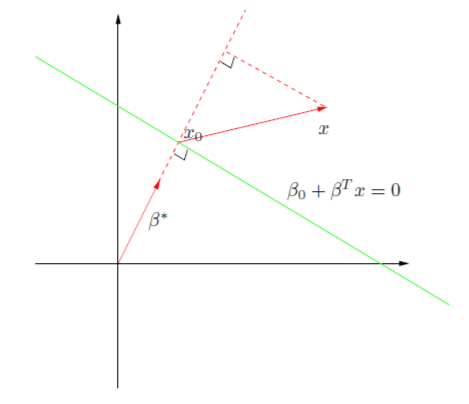
\includegraphics[width=.4\textwidth]{./chap/1chap/3sec/8images/1_hyperplaneAffine.PNG}
	\end{center}
	\caption{The linear algebra of a hyperplane (affine set)}
	\label{fig:1_hyperplaneAffine}
\end{figure}

\paragraph{Rosenblatt's Perceptron Learning Algorithm}
\tB{It tries to find a separating hyperplane by minimizing the distance of misclassified points 
to the decision boundary.} The goal is to minimize: 
%$$ D(\beta, \beta_{0}) = \su{{i\in\mathcal{M}}}{}y_{i}\left(x_{i}^{T}\beta + \beta_{0}\right)$$
\begin{center}
\enc{$D(\beta, \beta_{0}) = \su{{i\in\mathcal{M}}}{}y_{i}\left(x_{i}^{T}\beta + \beta_{0}\right)$}
\end{center}
where $\mathcal{M}$ indexes the set of misclassified points.

\begin{align*}
	\dfrac{\partial D(\beta,\beta_{0})}{\partial\beta}=&-\su{{i\in\mathcal{M}}}{}y_{i}x_{i}\\
	\dfrac{\partial D(\beta,\beta_{0})}{\partial\beta_{0}}=&-\su{{i\in\mathcal{M}}}{}y_{i}\\
\end{align*}
The algorithm in fact uses \tB{\textit{stochastic gradient descent}} to minimize this piecewise 
linear criterion.\\
The misclassified observations are visited in some sequence, and parameters $\beta$ are updated
via:
$${{\beta}\choose{\beta_{0}}} \leftarrow {{\beta}\choose{\beta_{0}}}+\rho {{y_{i}x_{i}}\choose{y_{i}}}$$
$\rho$ is the learning rate.

\paragraph{Optimal Separating Hyperplanes}
The \textit{optimal separating hyperplanes} separates the 2 classes and maximizes the distance
to the closet point from  either class. Consider the optimization problem:
\begin{center}
$\max\limits_{\beta,\beta_{0},\norm{\beta}=1} M$\\
subject to $y_{i}\left(x_{i}^{T}\beta+\beta_{0}\right)\geq M, i\in\inter{1}{N}$
\end{center}
\sB{The set of conditions ensure that all the points are at least a signed distance $M$ from the
decision boundary defined by $\beta$ and $\beta_{0}$}

%\subsection{Lab: logistic regression LDA, QDA and KNN}
%\begin{itemize}
 \item
 \end{itemize}

%%\subsection{Exercises}
%%\begin{itemize}
 \item
 \end{itemize}


\section{Resampling Methods}
\begin{itemize}
	\item
 \end{itemize}
\subsection{Cross-validation}
\begin{itemize}
	\item
 \end{itemize}

\subsection{The Bootstrap}
\tR{It can be used to quantify the uncertainity associated with a given
estimator or statistical learning method.}\\

\begin{figure}[H]
	\begin{center}
		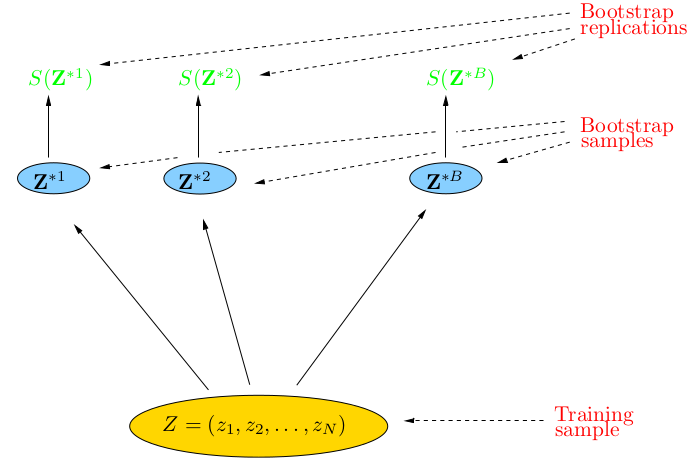
\includegraphics[width=.7\textwidth]{./chap/1chap/4sec/3_bootstrap.png}
	\end{center}
	\caption{Schematic of the bootstrap process}
	\label{fig:3_bootstrap}
\end{figure}

The basic idea is to randomly draw datasets with replacement from the training data, each sample
the same size as the original training set. This is done $B$ times, producing $B$ bootstrap datasets.
$S(\bm{Z})$ is any quantity computed from the data $\bm{Z}$. From the bootstrap sampling we can
estimate any aspect of the distribution of $S(\bm{Z})$, for example its variance:
\begin{center}
\enc{
$\hat{\V{S(\bm{Z})}}=\dfrac{1}{B-1}\su{{b=1}}{B}\left(S(\bm{Z}^{*b})-\overline{S}^{*}\right)^{2}$}
\end{center}
with $\overline{S}^{*}=\dfrac{1}{B}\su{{b=1}}{B}S(\bm{Z}^{*b})$
%\tB{We wish to minimize $\V{\alpha X+(1-\alpha)Y}$ (the risk)} one can
%show that the value that minimze the risk is : 
%\begin{center}
%\encV{$
%\alpha = \dfrac{\sigma_{Y}^{2}-\sigma_{XY}}{\sigma_{X}^{2}\sigma_{Y}^{2}-2\sigma_{XY}}
%$}
%\end{center}
%and $\sigma_{XY}=Cov(X,Y)$\\
%In reality, the quantities $\sigma_{X}^{2},\sigma_{Y}^{2}$ and $\sigma_{XY}$ are unknown.\\
%
%\tB{We can compute the standard error of these bootstrap estimates}
%using the formula:
%\begin{center}
%\encV{$
%SE_{B}\left( \hat{\alpha} \right)=
%\sqrt{\dfrac{1}{B-1}\su{{r=1}}{B}\left( \hat{\alpha}^{*r}-\dfrac{1}{B}\su{{r'=1}}{B}\hat{\alpha}^{*r'} \right)^{2}}
%$}
%\end{center}

\subsection{lab: Cross-validation and the Bootsrap}
\begin{itemize}
 \item
 \end{itemize}

\subsection{Exercises}
\begin{itemize}
 \item
 \end{itemize}


\section{Linear model selection and regularization}
\begin{itemize}
	\item
 \end{itemize}
\subsection{Subset selection}
\begin{itemize}
	\item
 \end{itemize}

\subsection{Shrinkage methods}
\paragraph{Ridge Regression}
\subparagraph{Definition}
\sB{The ridge regression coefficient estimates $\hat{\beta}^{R}$ are 
the values that minimize}:
\begin{center}
\encV{$
\su{{i=1}}{n}\left( y_{i}-\beta_{0}-\su{{j=1}}{p}\beta_{j}x_{ij} \right)^{2} + \lambda\su{{j=1}}{p}\beta_{j}^{2}=RSS+\lambda\su{{j=1}}{p}\beta_{j}^{2}
$}
\end{center}
where $\lambda > 0$ is a \emph{turning parameter} to be determined 
separately.\\
$RSS(\lambda)=(\bm{y}-\bm{X}\beta)^{T}(y-\bm{X}\beta)+\lambda\beta^{T}\beta$\\
\begin{center}
	\enc{$\hat{\beta}^{ridge}=(\bm{X}^{T}\bm{X}+\lambda\bm{I})^{-1}\bm{X}^{T}\bm{y}$}
\end{center}
In the case of orthonormal inputs, the ridge estimates are just a
scaled version of the least squares estimates, that is 
\tB{$\hat{\beta}^{ridge}=\frac{1}{1+\lambda}\hat{\beta}$}\\
The \tR{Singular Value Decomposition (SVD)} of the centered input matrix
$\bm{X}$ gives us some additional insight into the nature of ridge 
regression:
The $SVD$ of the $N\times p$ matrix $\bm{X}$ has the form:
\begin{center}
	\encB{$\bm{X} = \bm{UD}\bm{V}^{T}$}
\end{center}
Here \sB{$\bm{U}$ and $\bm{V}$ are $N\times p$ and $p\times p$ orthogonal
matrices}, with the columns of \sB{$\bm{U}$ spanning the columns space} of
$\bm{X}$, and the columns of \sB{$\bm{V}$ spanning the row space}.\\
$\bm{D}$ is a $p\times p$ diagonal matrix, containing singular values
of $\bm{X}$
Using the singular value decomposition:
\begin{align*}
	\bm{X}\hat{\beta}^{ls} &= \bm{X}(\bm{X}^{T}\bm{X})^{-1}\bm{X}^{T}\bm{y}\\
	&= \bm{U}\bm{U}^{T}\bm{y}
\end{align*}
For ridge regression:
\begin{align*}
	\bm{X}\hat{\beta}^{ridge} &= \bm{X}(\bm{X}^{T}\bm{X}+\lambda\bm{I})^{-1}\bm{X}^{T}\bm{y}\\
	&= \bm{U}\bm{D}(\bm{D}^{2}+\lambda\bm{I})^{-1}\bm{D}\bm{U}^{T}\bm{y}\\
	&= \su{{j=1}}{p}u_{j}\dfrac{d_{j}^{2}}{d_{j}^{2}+\lambda}u_{j}^{T}\bm{y}
\end{align*}
Like linear regression, \sB{ridge regression computes the coordinates of 
$\bm{y}$ with respect to the orthonormal basis $\bm{U}$, It shrinks
these coordinates by} \tB{$\dfrac{d_{j}^{2}}{d_{j}^{2}+\lambda}$}, a greater
amount of shrinkage is applied to the coordinates of basis vectors with
smaller $d_{j}^{2}$\\
The SVD of the centered matrix $X$ is another way to express the 
principal components of the variables in $\bm{X}$. The sample 
covariance matrix is given by $\bm{S}=\dfrac{\bm{X}^{T}\bm{X}}{N}$
\begin{center}
	$\bm{X}\bm{X}^{T}=\bm{V}\bm{D}^{2}\bm{V}^{T}$
\end{center}
which is the eigen decomposition of $\bm{X}^{T}\bm{X}$\\
The eigenvectors $v_{j}$ are also called the principal components 
directions of $\bm{X}$. The first principal component direction 
$v_{1}$ has the property that $z_{1}=\bm{X}v_{1}$ has the largest
sample variance amongst all normalized linear combinations of the 
columns of $\bm{X}$:
\begin{center}
	$\V{z_{1}}=\V{\bm{X}v_{1}}=\dfrac{d_{1}^{2}}{N}$
\end{center}
\begin{figure}[H]
	\begin{center}
		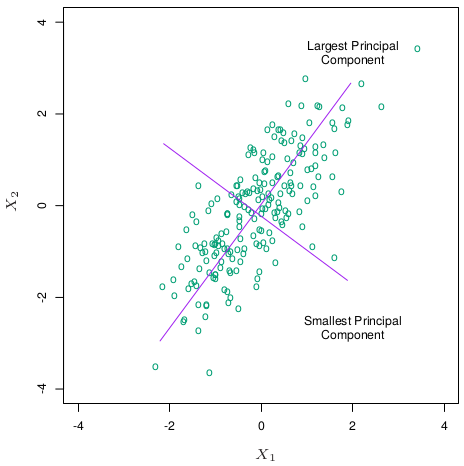
\includegraphics[width=.5\textwidth]{./chap/1chap/5sec/images/4_PrincipalComponentsRidge.png}
	\end{center}
	\caption{The largest principal components is the direction that
	maximizes the variance of the projected data and the smallest
	principal component minimizes that variance.
	\tB{Ridge regression projects $\bm{y}$ onto these components, and 
	then shrinks the coefficients of the low-variance components 
	more than the high-variance components}}
	\label{fig:5.4_PrincipalComponentsRidge}
\end{figure}
\begin{align*}
	df(\lambda) &=tr\left(\bm{X}(\bm{X}^{T}\bm{X}+\lambda\bm{I})^{-1}\bm{X}^{T}\right)\\
	&= tr(\bm{H}_{\lambda})\\
	&= \su{{j=1}}{p}\dfrac{d_{j}^{2}}{d_{j}^{2}+\lambda}
\end{align*}
This monotone decreasing function of $\lambda$ is the \emph{effective
degrees of freedom} of the ridge regression fit.\\
Note that \tB{$df(\lambda)=p$ when $\lambda=0$ (no regularization) and
$df(\lambda)\rightarrow 0$ as $\lambda\rightarrow \infty$}

\subparagraph{Why does Ridge Regression improve over Least Squares?}
Ridge regression's advantage over least squares is rooted in the 
\emph{bias-variance trade-off}. \tR{As $\lambda$ increases, the 
flexibility of the ridge regression fit decreases, leading to decreased
variance but increased bias.}

\begin{python}
reg = linear_model.Ridge(alpha=0.5)
reg.fit([[0, 0], [0, 0], [1, 1]], [0, 1, 1])
print(reg.coef_)
\end{python}
\paragraph{The Lasso}
It is a relatively recent alternative to ridge regression.\\
\sB{The Lasso coefficients, $\hat{\beta}_{\lambda}$ minimize the
quantity}:
\begin{center}
\encV{
$
\su{{i=1}}{n}\left( y_{i}-\beta_{0}-\su{{j=1}}{p}\beta_{j}x_{ij} \right)^{2}+\lambda\su{{j=1}}{p}|\beta_{j}| = RSS +\lambda\su{{j=1}}{p}|\beta_{j}|
$}
\end{center}
\tB{Models generated from the lasso are generally much easier to 
interpret than those produced by ridge regression.}
\begin{python}
reg = linear_model.Lasso(alpha=0.1)
reg.fit([[0, 0], [1, 1]], [0, 1])
print(reg.coef_)
\end{python}

\subparagraph{Another formulation for Ridge Regression and the Lasso}
\begin{center}
\encV{
$
\begin{cases}
	\min\limits_{\prtH{\beta}{j}{0}{p}}\left\{ \su{{i=1}}{n}\left( y_{i-}-\beta_{0}-\su{{j=1}}{p}\beta_{j}x_{ij} \right)^{2} \right\}\text{ subject to }\su{{j=1}}{p}|\beta_{j}|\leq s\text{ Ridge Regression}\\
	\min\limits_{\prtH{\beta}{j}{0}{p}}\left\{ \su{{i=1}}{n}\left( y_{i-}-\beta_{0}-\su{{j=1}}{p}\beta_{j}x_{ij} \right)^{2} \right\}\text{ subject to }\su{{j=1}}{p}\beta_{j}^{2}\leq s\text{ Lasso}
\end{cases}
$}
\end{center}

\paragraph{The variable selection property of the Lasso}
The least squares solution is marked as $\hat{\beta}$.
\begin{figure}[H]
	\begin{center}
		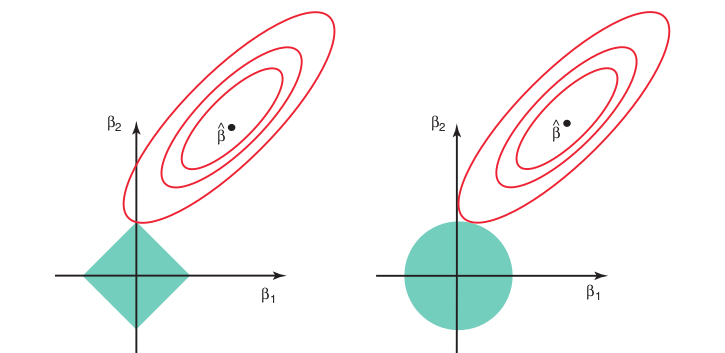
\includegraphics[width=\textwidth]{./chap/1chap/5sec/images/1RSSelipses.png}
	\end{center}
	\caption{Contours of the error and constraint functions for the
	lasso (left) and ridge regression (right). The solid blue areas
	are the constraint regressions, $|\beta_{1}|+|\beta_{2}|\leq 
	s\text{ and }\beta_{1}^{2}+\beta_{2}^{2}\leq s$, while the red
	ellipses are the contours of the RSS (all of the points on a
	given ellipse share a common value of the RSS).}
	\label{fig:5.1 RSSelipses}
\end{figure}

\sB{Since ridge regression has a circular contraint with no sharp
points, this intersection will not generally occur on an axis, and so
the
ridge regression coefficient estimates will be exclusively non-zero.}\\
However, the lasso constraint has \emph{corners} at each of the axes, 
and so the ellipse will often intersect the constraint region at an 
axis.

\subparagraph{Comparing the Lasso and Ridge Regression}
In general, one might expect \tB{the lasso to perform better in a
setting where a relatively small number of predictors have a 
substantial coefficients}, and the remaining predictors have 
coefficients that are very small or that equal zero.\\
\tB{Ridge regression will perform better when the response is a
function of many predictors}, all with coefficients of roughly equal 
size.\\

\tR{A technique such as cross-validation can be used in order to
determine which approach is better on a particular data set.}

\subparagraph{Bayesian Interpretation}
\tB{It assumes that the coefficient vector $\beta$ has some \emph{
prior} distribution}, say $p(\beta)$, where $\beta=
\begin{pmatrix}
	\beta_{0}\\
	.\\
	.\\
	.\\
	\beta_{p}
\end{pmatrix}
$
The likelihood of the data can be written as $f(Y|X,\beta)$, where
$X=
\begin{pmatrix}
	X_{1}\\
	.\\
	.\\
	.\\
	X_{p}
\end{pmatrix}
$
\sB{Multiplying the prior distribution by the likelihood gives us (up to a
proportionality constant) the posterior distribution} which takes the
form:\\
$
p(\beta|X,Y)\propto f(Y|X,\beta)p(\beta|X)=f(Y|X,\beta)p(\beta)
$\\
We assume that $Y=\beta_{0}+\su{{i=1}}{p}X_{i}\beta_{i}+\epsilon$ and:
$p(\beta)=\prd{{j=1}}{p}g(\beta_{j})$, for some density function $g$.\\
$g\hookrightarrow\mathcal{N}(0,f(\lambda)^{2})\Rightarrow$ the most
likely value for $\beta$ is given by the \emph{Ridge Regression} 
solution\\
$g\hookrightarrow Laplace(0,f(\lambda))\Rightarrow$ the posterior mode
for $\beta$ is the \emph{Lasso Regression} solution.
\begin{figure}[H]
	\begin{center}
		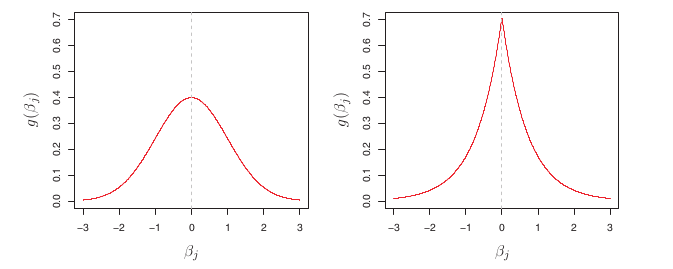
\includegraphics[width=\textwidth]{./chap/1chap/5sec/images/2bayesianPointOfView.png}
	\end{center}
	\caption{Left: Ridge regression is the posterior mode for 
	$\beta$ under a Gaussian prior.\\
	Right: The lasso is the posterior mode for $\beta$ under a 
	double-exponential prior.}
	\label{fig:2bayesianPointOfView}
\end{figure}
We can generalize ridge regression and the lasso, and view them as 
Bayes estimates:
\begin{center}
	\enc{
	$\tilde{\beta}=\min\limits_{\beta}\left\{
	\su{{i=1}}{N}\left(y_{i}-\beta_{0}-
	\su{{j=1}}{p}x_{ij}\beta_{j}\right)^{2}+
	\lambda\su{{j=1}}{p}|\beta_{j}|^{q}\right\}$}
\end{center}
for $q\geq 0$
The value:
$
\begin{cases}
	q=0:\text{ \emph{subset selection} the penalty
	counts the number of nonzero parameters}\\
	q=1:\text{ the \emph{lasso}}\\
	q=2:\text{ the \emph{ridge regression}}
\end{cases}
$\\
The case $q=1$ (lasso) is the smallest $q$ such that the constraint
region is convex: \sV{non-convex constraint regions make the optimization
problem more difficult}.
\begin{figure}[H]
	\begin{center}
		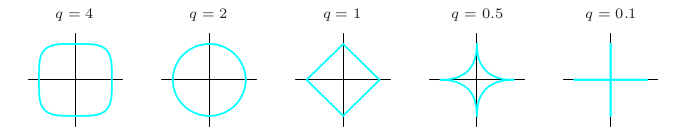
\includegraphics[width=.7\textwidth]{./chap/1chap/5sec/images/5_penaltyContours.png}
	\end{center}
	\caption{Contours of constant value of 
	$\su{j}{}|\beta_{j}|^{q}$}
	\label{fig:5.5_penaltyContours}
\end{figure}
\paragraph{Elastic-net}
\begin{center}
	\enc{$\lambda\su{{j=1}}{p}\left(\alpha\beta_{j}^{2}+(1-\alpha)|\beta_{j}|\right)$}
\end{center}
\begin{python}
reg = linear_model.ElasticNet(random_state=0)
reg.fit([[0, 0], [1, 1]], [0, 1])
print(reg.coef_)
\end{python}

\paragraph{Selecting the Tuning Parameter}
Cross-validation provides a simple way to select $\lambda$ or 
equivalently $s$:\\
\begin{itemize}
	\item We choose a grid of $\lambda$ values
	\item We compute the cross-validation for each value of 
		$\lambda$
	\item We select the tuning parameter value for which the 
		cross-validation error is smallest.
\end{itemize}
Finally the model is re-fit using all of the available observations and
the selected value of the tuning parameter.
\begin{python}
X, y = load_diabetes(return_X_y=True)
clf = RidgeCV(cv = 5, random_state=0).fit(X, y)
print(clf.alpha_)

clf = LassoCV(cv = 5, random_state=0).fit(X, y)
print(clf.alpha_)

clf = ElaticNet(cv = 5, random_state=0).fit(X, y)
print(clf.alpha_) # corresponds to lambda
print(clf.l1_ratio_) # corresponds to alpha
\end{python}

\paragraph{Least Angle Regression}
\subparagraph{Least Angle Regression}
\begin{enumerate}
	\item \sB{Standardize the predictors} to have mean zero an unit 
		norm.\\ \sB{Start with the residual $\bm{r}=\bm{y}-
		\overline{\bm{y}}$}, and for all $i\in\inter{1}{p}
		\beta_{i}=0$
	\item Find the predictor $x_{j}$ most correlated with $\bm{r}$
	\item Move $\beta_{j}$ from 0 to its least-squares coefficient
		$\dfrac{\sP{\bm{x}_{j}}{\bm{r}}}{\sP{\bm{x}_{j}}{\bm{x}_{j}}}$, then recompute 
		$\bm{r}$. Find the predictor $x_{k}$ most correlated with the new $\bm{r}$
	\item Move $\beta_{k}$ from 0 to its least-squares coefficient
		$\dfrac{\sP{\bm{x}_{k}}{\bm{r}}}{\sP{\bm{x}_{k}}{\bm{x}_{k}}}$, then recompute 
		$\bm{r}$. Find the predictor $x_{l}$ most correlated with the new $\bm{r}$\dots
%	\item Move $\beta_{j}$ and $\beta_{k}$ in the direction defined
%		by their joint least squares coefficient of the current
%		residual on $(x_{j},x_{k})$, until some other 
%		competitor $x_{l}$ has as much correlation with the
%		current residual.
	\item Continue in this way until all $p$ predictors have been
		entered. After $\min(N-1, p)$ steps, we arrive at the
		full least-squares solution.
\end{enumerate}
Suppose $\mathcal{A}_{k}$ is the active set of variables at the 
beginning of the $k^{th}$ step and let $\beta_{\mathcal{A}_{k}}$ be the
coefficient vector for these variables at this step, there will be 
$k-1$ nonzero values and the one just entered will be zero.\\
If \sB{$\bm{r}_{k}=\bm{y}-\bm{X}_{\mathcal{A}_{k}}\beta_{\mathcal{A}_{k}}$}
is the current residual, then the direction for this step is:
\begin{center}
	$\delta_{k}=(\bm{X}_{\mathcal{A}_{k}^{T}}\bm{X}_{\mathcal{A}_{k}^{T}})^{-1}\bm{X}_{\mathcal{A}_{k}^{T}}^{T}\bm{r}_{k}$
\end{center}
The name ``least angle'' arises from a geometrical interpretation of 
this process; $\bm{u}_{k}$ makes the smallest (and equal) angle with
each of the predictors in $\mathcal{A}_{k}$
Advantages and Disadvantages:
\begin{itemize}
	\item[\tV{+}] Numerically efficient when $p\gg n$
	\item[\tV{+}] As fast as forward selection and has the same order of complexity as OLS
	\item[\tV{+}] Produces a full piecewise linear solution path
	\item[\tV{+}] Stable
	\item[\tV{+}] Esealy modified to produce for other estimators like the Lasso
	\item[\tR{-}] Because LARS is based upon iterative refitting of the residuals, it would
		appears to be especially sensitive to the effect noise.
\end{itemize}

\subparagraph{Least Angle Regression: Lasso Modification}
\begin{itemize}
	\item[4a] If a non-zero coefficient hits zero, drop its variable from the
		active set of varibalbes and recompute the current joint least squares
		direction
\end{itemize}
\begin{python}
reg = Lars()
reg.fit([[ -1, 1], [0, 0], [1, 1]], [-1.1111, 0, -1.1111])
print(reg.coef_)
\end{python}

\subsection{Dimension reduction methods}
\paragraph{Principal Component Analysis}
\subparagraph{Intuitive}
PCA can be thought of as \tB{fitting a $p-dimensional$ to the data, which each axis of the
ellipsoid represents a principal component}. If some axis of the ellipsoid is small, then the
variance along that axis is also small, and by omitting that axis and its corresponding principal
component from our representation of the dataset. 

\subparagraph{Methods}
To find the axes ellipsoid, we must first subtract the mean of each variable from the dataset
to center the data around the origin. 
\begin{enumerate}
	\item \sB{Subtract the mean of each variable} from the dataset to center the data around 
		the origin.
	\item \sB{Computing the covariance matrix} of the data and \sB{calculate the eigenvalues} and
		corresponding eigenvectors.
	\item \sB{Normalize each of the orthogonal eigenvectors} to turn into unit vectors.
\end{enumerate}
Then each of the mutually orthogonal, unit eigenvectors can be interpreted as an axis of the 
ellipsoid fitted to the data.\\ Our covariance matrix will be transformed into a diagonalised
form with the diagonal elements representing the variance of each axis.\\
The proportion of the variance that each eigenvector represents can be calculated by dividing 
the eigenvalue corresponding to that eigenvector by the sum of all eigenvalues.

\subparagraph{Mathematically}
PCA is defined as an orthogonal linear transformation that transforms the data to a new
coordinate system such that the greatest variance by some scalar projection of the 
data comes to lie on the first coordinate (the first principal component), the second greatest
variance on the second coordinate.\\

The transformation is defined by a \sB{set of size $l$ of $p-dimensional$ vectors of weights}
$\bm{\omega}_{(k)}=(\omega_{1},\cdots,\omega_{p})_{(k)}$, with $k\in\inter{1}{l}$, \sB{that map each
row vector} $\bm{x}_{(i)}$ of $\bm{X}$ \sB{to a new vector of principal component scores} $t_{(i)}=
(t_{1}, \cdots, t_{l})_{(i)}$ given by:
$\forall(i,k)\in\inter{1}{n}\times\inter{1}{l}{t_{k}}_{(i)}=\sP{\bm{x}_{i}}{\bm{\omega}_{(k)}}
\text{ with }l\leq p$\\

\tB{In order to maximize variance}, the first weight vector $\bm{\omega}_{(1)}$ thus has to satisfy:
\begin{center}
$\bm{\omega}_{(1)} = \max\limits_{\norm{\bm{\omega}}=1}\norm{\bm{X}\bm{\omega}}^{2}=
\max\limits_{\norm{\bm{\omega}}=1}\left(\bm{X}\bm{\omega}\right)^{T}\bm{X}\bm{\omega}$
\end{center}
Since $\bm{\omega}_{(1)}$ has been defined to be a unit vector, it equivalently also satisfies:
\begin{center}
\enc{$\bm{\omega}_{(1)}=\max\limits_{\norm{\bm{\omega}}=1}\dfrac{\bm{\omega}^{T}\bm{X}^{T}\bm{X}\bm{
\omega}}{\bm{\omega}^{T}\bm{\omega}}$}
\end{center}
The quantity to be maximised can be recognized as a Rayleigh quotient. A standard result \sB{for a 
positive semidefinite matrix such as $\bm{X}^{T}\bm{X}$ is that the Rayleigh quotient's maximum
possible value is the largest eigenvalue of the matrix, which occurs when $\bm{\omega}$ is the 
corresponding eigenvector}.\\

\textbf{\emph{Further components}}:\\
The $k^{th}$ component can be found by subtracting the first $k-1$ principal components from
$\bm{X}$:
\tB{$\hat{\bm{X}}_{k}=\bm{X}-\su{{s=1}}{k-1}\bm{X}\bm{\omega}_{(s)}\bm{\omega}_{(s)}^{T}$}
and then finding the weight vector which extracts the maximum variance from this new data matrix:
\begin{center}
\encB{$\bm{\omega}_{(k)}=\max\limits_{\norm{\bm{\omega}}=1}\norm{\hat{\bm{X}}_{k}\bm{\omega}}^{2}=
\max\limits_{\norm{\bm{\omega}}=1}\dfrac{\bm{\omega}^{T}\hat{\bm{X}}_{k}^{T}\hat{\bm{X}}_{k}\bm{
\omega}} {\bm{\omega}^{T}\bm{\omega}}$}
\end{center}
It turns out that this gives the remaining eigenvectors of $\bm{X}^{T}\bm{X}$, with the maximum 
values for the quantity in brackets given by their corresponding eigenvalues. Thus the weight vectors
are eigenvectors of $\bm{X}\bm{X}^{T}$.\\
The \sR{full principal components decomposition of $\bm{X}$ can therefore be given as:
$\bm{T}=\bm{X\Omega}$}
where \tR{$\bm{\Omega}$ is a $p\times p$ of weights whose columns are the eigenvectors of 
$\bm{X}^{T}\bm{X}$}.

\begin{figure}[H]
	\begin{center}
		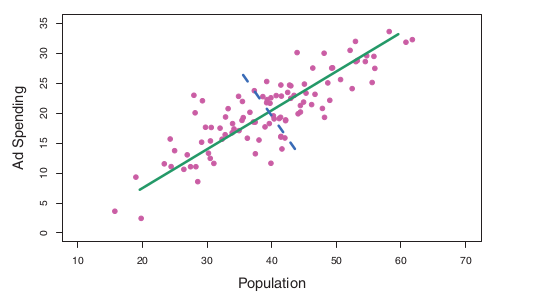
\includegraphics[width=\textwidth]{./chap/1chap/5sec/images/3principalCompoment.png} \end{center}
	\caption{The population size and ad spending for 100 different
	cities are shown as purple circles. The green solid line
	indicates the first principal component, and the blue dashed
	line indicates the second principal compoment.}
	\label{fig:3principalCompoment}
\end{figure}

\subparagraph{Principal Components Regression and Ridge Regression}
The \emph{Principal Components Regression} (PCR) approach \tB{involves
constructing the first $M$ principal components $\prth{Z}{i}{M}$
and then using these components as the predictors in a linear 
regression model that is fit using least squares}.\\

One can show that PCR and Ridge Regression are very closely related, 
one can even think of ridge regression as a continuous version of PCR.
\\
When performing PCR we generally recommend \emph{standardizing} each
predictor, using, prior to generating the principal components.\\

Ridge regression shrinks the coefficients of the principal components,
shrinking more depending on the size of the corresponding eigenvalue;
principal components regression discard the $p-M$ smallest eigenvalue
components.\\
\subparagraph{Python Code}
\begin{python}
import numpy as np
import pandas as pd
import matplotlib.pyplot as plt
import statsmodels.api as sm
from statsmodels.multivariate.pca import PCA
import sklearn
from sklearn.preprocessing import StandardScaler
from sklearn.decomposition import PCA as PCA_sk

df = pd.read_csv('myfile.csv', sep=';')
X, y = df.iloc[:, 1:], df.iloc[:, 0]
pca_model = PCA(X,
    standardize=False, # mean 0 and unit variance
    demean=True # to subtract columns by their mean
)
# Standardize the Data
fig = pca_model.plot_scree(log_scale=False) # to plot the explained
# variance of components.
print(pca_model.loadings.iloc[:, :2]).argsort() # to
# estimate the implication of a given variable in a the
# 2 first components.

# Computation
X_rm_mean = StandardScaler(with_std=False).fit_transform(X)
pca = PCA_sk(n_components=2) # 2 assuming that the 2 first 
# principal components explained the quasi-totality of the variance
principalCompnents = pca.fit_transform(X_rm_mean)
df_pca = pd.DataFrame(data= principalCompnents,
    columns=['pc1', 'pc2'])
df_transf = df.iloc[:, 0].join(df_pca)

# Visualize
fig = plt.figure()
ax.set_xlabel('Principal Component 1', fontsize=15)
ax.set_ylabel('Principal Component 2', fontsize=15)
ax.set_title('2 component PCA', fontsize=20)
ax.scatter(df_transf.loc[:, 'pc1'], df_transf.loc[:, 'pc2'])

# Explained Variance
print(pca.explained_variance_ratio_)
\end{python}

\paragraph{Partial Least Squares}
\tB{It is a \emph{supervised} alternative to PCR, PLS approach attempts
to find directions that help explain both the response and the
predictors.}\\
\begin{itemize}
	\item To standardize the $p$ predictors
	\item Computation of the first direction $Z_{1}$ by setting 
		each $\phi_{j1}$ equal to the coefficient from the
		simple linear regression of $Y$ onto $X_{j}$.
\end{itemize}
Hence in computing $Z_{1}=\su{{j=1}}{p}\phi_{j1}X_{j}$ places the 
highest weight on the variables that are most strongly related to the
response.
\subparagraph{Partial Least Squares}
\begin{itemize}
	\item Standardize each $x_{j}$ to have mean zero and variance
		one.\\ Set $\hat{\bm{y}}^{(0)}=\overline{\bm{y}}$ and
		for all $j\in\inter{1}{p}~x_{j}^{(0)}=x_{j}$ 
	\item For $m\in\inter{1}{p}$
		\begin{enumerate}[label=(\alph*)]
			\item $\bm{z}_{m}=\su{{j=1}}{p}\dfrac{\sP{\bm{x}_{j}^{(m-1)}}{\bm{y}^{(m-1)}}
				}{\sP{\bm{x}_{j}^{(m-1)}}{\bm{x}_{j}^{(m-1)}}}\bm{x}_{j}^{(m-1)}$
			\item $\hat{\bm{y}}^{(m)} = 
				\hat{\bm{y}}^{(m-1)} + 
				\dfrac{\sP{\bm{z}_{m}}{\bm{y}^{(m-1)}}}{\sP{\bm{z}_{m}}{\bm{z}_{m}}}\bm{z}_{m}$
			\item Orthogonalize each $\bm{x}_{j}^{m-1}$ 
				with respect to $\bm{z}_{m}$:\\
				$\bm{x}_{j}^{(m)}=\bm{x}_{j}^{(m-1)}-
				\dfrac{\sP{\bm{z}_{m}}{\bm{x}_{j}^{(m-1)}}}{\sP{\bm{z}_{m}}{\bm{z}_{m}}}\bm{z}_{m}$ for $j\in\inter{1}{p}$
		\end{enumerate}
\end{itemize}
\sB{PLS seeks directions that havae high variance and have high correlation with response,
in contrast to PCR which keys only on high variance.}
Particularly  the $m^{th}$ principal component direction $v_{m}$ solves:
$$ \max_{\alpha} \V{\bm{X}\alpha} \text{such that}
\begin{cases} 
	\norm{\alpha}=1 \\ 
	\forall l\in \inter{1}{m-1} \alpha^{T}\bm{S}v_{l} = 0
\end{cases}$$
$\bm{S}$ is the sample covariance matrix of the $\bm{x}_{j}$
The conditions $\alpha^{T}\bm{S}v_{l}=0$ ensures that $z_{m} = \bm{X}\alpha$ is 
uncorrelated with all the previous linear combinations $z_{f}=\bm{X}v_{l}$\\
The $m^{th}$ PLS direction $\hat{\Phi}_{m}$ solves 
$$ \max_{\alpha} Corr^{2}(\bm{y}, \bm{X\alpha})\V{\bm{X}\alpha} \text{such that}
\begin{cases} 
	\norm{\alpha}=1 \\ 
	\forall l\in \inter{1}{m-1} \alpha^{T}\bm{S}\hat{\Phi}_{l} = 0
\end{cases}$$

\sB{PLS, PCR and Ridge Regression tend to behave similarly, Ridge Regression may be 
preferred because it shrinks smoothly}, rather than in discrete steps. Lasso falls
somewhere between ridge regression and best subset regression, and enjoys some of the
properties of each.

\subparagraph{Python Code}
\begin{python}
X = [[0., 0., 1.], [1., 0., 0.], [2., 2., 2.], [2., 5., 4.]]
y = [0.1, 0.9, 12.3]

pls1 = PLSRegression(n_components=2)
pls1.fit(X, y)
print(pls1.score(X, y))
\end{python}


\subsection{Consideration in high dimensions}
\paragraph{High-Dimensional Data}
Data sets containing more features than observations are often referred
to as \emph{high-dimensional}. \sB{Classical approaches such as least 
squares linear regression are not appropriate in this setting.}

%\paragraph{What goes wrong in high dimensions?}
%Regression and classification when $p>n$, we begin by examining what
%can go wring if we apply a statistical technique not intended for the
%high-dimensional setting.

\paragraph{Regression in High Dimensions}
\sB{Ridge regression, the lasso and principal components regression, are
particularly useful} for performing regression in the high-dimensional
setting. Essentially these approaches avoid overfitting by using a 
less flexible fitting approach than least squares.

%\paragraph{Interpreting Results in High Dimensions}
%At most, we can hope to assign large regression coefficients to 
%variables that are correlated with the variables that truly are 
%predictive of the outcome.

\subsection{Lab1: subset selection methods}
\begin{itemize}
 \item
 \end{itemize}

\subsection{Lab2: ridge regression and the Lasso}
\begin{itemize}
 \item
 \end{itemize}

\subsection{lab3: PCR and PLS regression}
\begin{itemize}
 \item
 \end{itemize}

\subsection{Exercises}
\begin{itemize}
 \item
 \end{itemize}


\section{Moving beyond linearity}
\subsection{Polynomial Regression}
\paragraph{Definition}
Historically when the relationship between the response and the
predictors is non-linear we used to replace the standard linear model
$$
y_{i}=\beta_{0}+\beta_{1}x_{i}+\epsilon_{i}
$$
with a polynomial function:
\begin{center}
\enc{$
y_{i}=\su{{r=0}}{d}\beta_{r}x_{i}^{r}
$}
\end{center}
Generally speaking, \tB{it is unusual to use $d$ greater than 3 or 4}.

\begin{python}
import pandas as pd
import sklearn
from sklearn.preprocessing import PolynomialFeatures
from sklearn.linear_model import LinearRegression
from sklearn.pipeline import Pipeline

df = pd.read_csv('myFile.csv', sep=';')
y, X = df.iloc[:, 0].values, df.iloc[:, 1].values.reshape(-1, 1)

model = Pipeline([
  ('poly', PolynomialFeatures(degree=3)),
  ('linear', LinearRegression(fit_intercept=False))
  ])
model = model.fit(X, y)
print(model.score(X, y))
\end{python}

%\subsection{Step functions}
%\begin{itemize}
	\item
 \end{itemize}

%%\subsection{Basis functions}
%%\begin{itemize}
 \item
 \end{itemize}

\subsection{Regression splines}
\paragraph{Piecewise Polynomials}
\tB{It involves fitting separate low-degree polynomials over different 
regions of $X$.}\\
The points where the coefficients change are called \tR{\emph{knots}}.
It is a function $f(X)$ that is obtained by dividing the domain of $X$ into contiguous intervals,
and representing $f$ by a separate polynomial in each interval.
More generally, an order$-M$ spline with knots $\zeta_{j}, j\in\inter{1}{K}$ is a 
piecewise-polynomial of order $M$, and has continuous derivatives up to order $M-2$.
Likewise the general form for the truncated-power basis set would be:
\begin{align*}
h_{j}(X) &= X^{j-1}, &j\in\inter{1}{M}\\
h_{M+j} &=\left(X-\zeta_{l}\right)_{+}^{M-1}, &l\in\inter{1}{K}
\end{align*}

%\paragraph{Constraints and Splines}
%We can fit a piecewise polynomial under the constraint that the fitted
%curve must be continuous.

\paragraph{The spline Basis Representation}
A cubic spline with $K$ knots can be modeled as:
\begin{center}
\enc{$
y_{i}=\beta_{0}+\su{{r=1}}{K+3}\beta_{r}b_{r}(x_{i})
$}
\end{center}
for an appropriate choice of \emph{basis functions} $\prth{b}{i}{K+3}$\\
The most direct way to represent cubic spline is \tB{to start off with
a basis for a cubic polynomial -namely, $x, x^{2}, x^{3}$ -and then add
one \emph{truncated power basis} function per knot}.
A truncated power basis function, for a cubic polynomial, is defined as:
\begin{center}
\enc{$
h(x,\zeta) = (x-\zeta)_{+}^{3}=
\left\{
\begin{array}{ll}
	(x-\zeta)^{3}&\mbox{if }x>\zeta\\
	0&\mbox{otherwise}
\end{array}
\right.
$}
\end{center}
where $\zeta$ is the knot.\\
In order to fit a cubic spline to a data set with $K$ knots, we perform
least squares regression with an intercept and $3+K$ predictors of the
form $X, X^{2}, X^{3}, h\left(X,\zeta_{1}\right), h\left(X,\zeta_{2}\right),,..,h\left(X,\zeta_{K}\right)$ where $\prth{\zeta}{i}{K}$ are the
knots. This amounts to estimating a total of $K+4$ regression 
coefficients.\\
Cubic splines are popular because most human eyes cannot detect 
discontinuity at the knots.

\begin{figure}[H]
	\begin{center}
		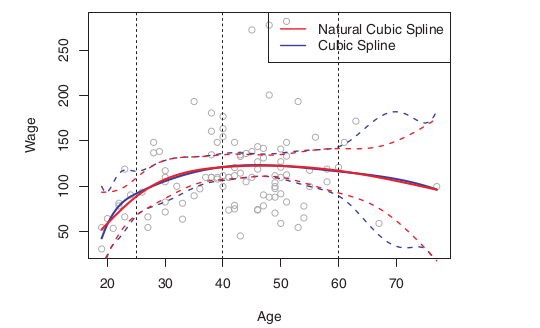
\includegraphics[width=.7\textwidth]{./chap/1chap/6sec/images/1splines.png}
	\end{center}
	\caption{A cubic spline and a natural cubic spline, with 3 
	knots, fit to a subset of the Wage data, confidence interval as
	dashed lines.}
	\label{fig:6.1splines}
\end{figure}
A natural spline is a regression spline with additional boundary 
constraints: the function is required to be linear at the boundary (in
the region where $X$ is smaller than the smallest knot, or larger than
the largest knot).\\
\tB{This frees up $4$ degrees of freedom ($2$ constraints each in both boundary regions), which
can be spent more profitably by sprinkling more knots in the interior region. }
A natural cubic spline with $K$ knots is represented by $K$ basis functions.
\begin{center}
	$\begin{cases}
		N_{1}(X) = 1\\
		N_{2}(X) = X
	\end{cases}
	,~ N_{k+2}(X) = d_{k}(X)-d_{K-1}(X)$
\end{center}
where $d_{k}(X) = \dfrac{\left(X-\zeta_{k}\right)_{+}^{3} - \left(X-\zeta_{K}\right)_{+}^{3}}{
\zeta_{K}-\zeta_{k}}$

\paragraph{Choosing the Number and Locations of the Knots}
One option is \tB{to place more knots in places where we feel the 
function might vary most rapidly}, and to place fewer knots where it 
seems more stable.\\
\sR{For the number of knots we can use cross-validation.}

\begin{python}
import pandas 
import statsmodels.api as sm
import sklearn
from sklearn.model_selection import KFold
import patsy
from patsy import dmatrix

# Choosing the good number of knots
y, x = df.iloc[:, 0], df.iloc[:, 1]
kf = KFold(n_splits=5)
n = 52
cv_set = {str(i):0 for i in range(1, n)}
for i in range(1, n):
    n_knots = i
    knot_list = np.quantile(x, np.linspace(0, 1, n_knots + 2))[1:-1]
    mse_list = []
    for train, test in kf.split(x):
        x_natural = dmatrix('cr(x, knots=knot_list)', {'x':x[train]})
        fit_natural = sm.GLM(y[train], x_natural).fit()
        yhat = fit_natural.predict(dmatrix('cr(x, knots=knot_list)', {'x':x[test]}))
        mse = ((yhat-y[test])**2).mean()
        # mse_list.append(mse)
        mse_list.append(mse)
        # print(mse)
    cv_set[str(i)] = np.array(mse_list).mean()
cv_list = list({k:v for k,v in sorted(cv_set.items(), key=lambda item: item[1])})


n_knots = int(cv_list[0])
knot_list = np.quantile(x, np.linspace(0, 1, n_knots + 2))[1:-1]
# Natural
x_natural = dmatrix('cr(x, knots = knot_list)', {'x':x})
fit_natural = sm.GLM(y, x_natural).fit()

# Create spline
xp = np.linspace(x.min(), x.max(), 50)
line_natural = fit_natural.predict(dmatrix('cr(xp,knots=knot_list)',
                                           {'xp':xp}))

plt.figure()
plt.scatter(df.iloc[:, 0], df.iloc[:, 1])
plt.plot(xp, line_natural, color='red', label="Natural Spline Regression")
for k in knot_list:
    plt.axvline(k, color='gray', ls='--')
plt.legend()
plt.show()
\end{python}
\paragraph{Comparison to Polynomial Regression}
Regression splines give superior results to polynomial regression.\\
\sB{This is because unlike polynomials, which must use a higher degree 
to produce flexible fits, splines introduce flexibility by increasing
the number of knots but keeping the degree fixed.}\\
Splines produce also more stable estimates.

\subsection{Smoothing splines}
\begin{itemize}
	\item
 \end{itemize}

\subsection{Local regression}
\paragraph{Span}
It plays a role like that of the tuning parameter $\lambda$ in 
smoothing splines: \tB{it controls the flexibility of the non-linear fit}.\\
\sT{The smaller the value of $s$, the more \emph{local} will be our fit.}

\paragraph{Algorithm: \emph{Local Regression} at $X=x_{0}$}
\begin{figure}[H]
	\begin{center}
		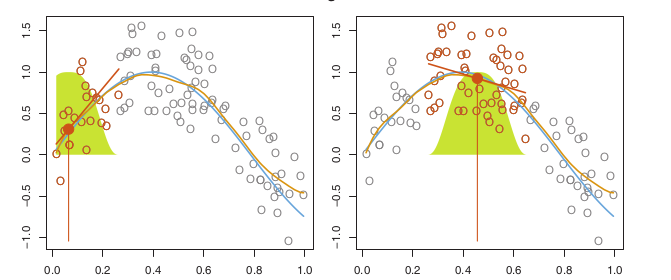
\includegraphics[width=\textwidth]{./chap/1chap/6sec/images/2localRegression.png}
	\end{center}
	\caption{Blue curve represents $f(x)$ from which the data were
	generated.\\
	Orange curve corresponds to the local regression estimate $f(x)$.\\
	Orange colored points are local to the target point $x_{0}$.\\
	Yellow-bell-shape superimposed on the plot indicates weights 
	assigned to each point, decreasing to zero with distance from
	the target point.}
	\label{fig:6.1localRegression}
\end{figure}
\begin{enumerate}
	\item Gather the fraction $s=\frac{k}{n}$ of training points
		whose $x_{i}$ are closet to $x_{0}$
	\item Assign a weight $k_{i0}=K(x_{i},x_{0})$ so that \tB{the
		point furthest from $x_{0}$ has weight zero, and the 
		closet has the highest weight}.\\
		\sB{All but these $k$ nearest neighbors get weight 0}
	\item \tB{Fit a weighted least squares regression of the $y_{i}
		$ on the $x_{i}$}, using the aforementioned weights, by
		\tB{finding $\beta_{0}$ and $\beta_{1}$ that minimize:
		$$\su{{i=1}}{n}K_{i0}(y_{i}-\beta_{0}-\beta_{1}x_{i})^{2}$$}
	\item \tB{The fitted value at $x_{0}$ is given by $\hat{f}(x_{
		0})= \hat{\beta}_{0}+\hat{\beta}_{1}x_{0}$}
\end{enumerate}
For $p$-dimensional neighborhoods, local regression can perform poorly
if $p$ is much larger than 3 or 4, because there will generally be very
few training observations close to $x_{0}$

\subsection{Generalized additive models}
\emph{Generalized Additive Models} (GAMs) \sB{provide a genral 
framework for extending a standard linear model by allowing non-linear}
functions of each of the varialbes, \sB{while maintaining additivity}.

\paragraph{Principle}
\subparagraph{Definition}
Considering we have $y_{i}=\beta_{0}+\su{{r=1}}{p}\beta_{r}x_{ir}+
\epsilon$\\ \tB{We replace each linear component $\beta_{j}x_{ij}$ with
a (smooth) non-linear function $f_{j}(x_{ij})$}:\\
$$
y_{i}=\beta_{0}+\su{{j=1}}{p}f_{j}(x_{ij})+\epsilon_{i}
$$
\sB{It is called an \emph{additive model} because we calculate a
separate $f_{i}$ for each $X_{j}$, and then add together all of their 
contributions.}\\
In the regression setting, a generalized additive model has the form: 
$\E{Y|\prth{X}{j}{p}}=\alpha+\su{{j=1}}{p}f_{j}(X_{j})$, the $f_{j}$'s are unspecified smooth
(``non-parametric'') functions.
\paragraph{Fitting Additive Models}
The additive model has the form:
\begin{center}
	\enc{$ Y = \alpha + \su{{j=1}}{p}f_{j}(X_{j})+\epsilon$}
\end{center}
where $\E{\epsilon}=0$. Given observations $x_{i},y_{i}$ a criterion like the penalized sum of
squares
\begin{center}
\encB{$ PRSS\left(\alpha,\prth{f}{j}{p}\right) = \su{{i=1}}{N}\left(y_{i}-\alpha-\su{{j=1}}{p}
f_{j}(x_{ij})\right)^{2} + \su{{j=1}}{p}\lambda_{j}\su{}{}f_{j}^{''}(t_{j})^{2}dt_{j}$}
\end{center}
where the $\lambda_{j}\geq 0$ are the tuning parameters.

\subparagraph{The Backfitting Algorithm for Additive Models}
\begin{enumerate}
	\item Initialize: $\forall (i,j)\in\inter{1}{N}\times\inter{1}{p}, \hat{\alpha} = \dfrac{1}{N}\su{{1}}{N}y_{i}, \hat{f}_{j}\equiv 0$
	\item Cycle: $j=1,\dots,p,1,\dots,p,\dots$
		\begin{align*}
			\hat{f}_{j} &\leftarrow \bm{S}_{j}\left[\left\{y_{i}-\hat{\alpha}-
			\su{{k\neq}}{}\hat{f}_{k}(x_{ik})\right\}_{1}^{N}\right]\\
			\hat{f}_{j} &\leftarrow \hat{f}_{j}-\dfrac{1}{N}\su{{i=1}}{N}\hat{f}_{j}(x_{ij})
		\end{align*}
		until the function $\hat{f}_{j}$ change less than a pre-specified threshold.
\end{enumerate}
We set \sB{$\hat{\alpha}=ave(y_{i})$} and it never changes. We apply a \sB{cubic smoothing spline  
$S_{j}$} to the targets $\left\{y_{i}-\hat{\alpha}-\su{{k\neq j}}{}\hat{f}_{k}(x_{ik})\right\}_{1}^{N
}$. The process is continued unitil the estimates $\hat{f_{j}}$ stabilize.\\ \sB{The backfitting 
procedure allow one to choose a fitting method appropriate for each input variable however it fits 
all predictors which is not feasible or desirable when a large number are available}

\subparagraph{Python Code}
\begin{python}
import pygam
from pygam import LinearGAM, LogisticGAM
from pygam import GAM, l, s, f, te, intercept


# REGRESSION
df_reg = pd.read_csv('myFile_reg.txt', sep=';')
y, X = df.iloc[:, 0], df.iloc[:, 1:]
p = len(X)
lgam = LinearGAM(
   eval(' + '.join(['f({})'.format(i) 
       for i in range(p-3)] +
       ['l(p-3)', 'l(p-2)', 'l(p-1)'])
       )
)

lgam_grid = lgam.gridsearch(X, y)
lgam_grid.summary()

fig, ax = plt.subplots()
ax.scatter(X.budget_std, y)
ax.plot(X.budget_std, lgam_grid.predict(X), color='red')
ax.plot(X.budget_std, lgam_grid.prediction_intervals(X)[:, 0])
ax.plot(X.budget_std, lgam_grid.prediction_intervals(X)[:, 1])
plt.show()



# CLASSIFICATION
# Replace LinearGAM by LogisticGAM!!

\end{python}

\subparagraph{Pros and Cons of GAM's}
\begin{itemize}
	\item[\tV{+}] We do not need to manually try out many different
		transformations on each variable individually.
	\item[\tV{+}] The non-linear fits can potentially make more
		accurate predictions for the response $Y$
	\item[\tV{+}] Because the model is additive, we can examine the
		effect of each $X_{j}$ on $Y$ individually while 
		holding all of the other variables fixed.
		
	\item[\tV{+}] The smoothness of the function $f_{j}$ for the 
		variable $X_{j}$ can be summarized via degrees of 
		freedom.
	\item[\tR{-}] The model is restricted to be additive
\end{itemize}

\paragraph{The Naive Bayes Classifier}
It is \tB{especially appropriate when dimension $p$ of the feature space is high}, making density 
estimation unattractive. The naive Bayes model \tB{assumes that given a class $G=j$, the features
$X_{k}$ are independent}.\\
While this assumption is generally not true, it does simplify the estimation dramatically, using
class $J$ as the base we can derive:
\begin{itemize}
	\item The individual class-conditional marginal densities $f_{jk}$ can each be estimated
		separately using one-dimensional kernel density estimates.
	\item If a component $X_{j}$ of $X$ is discrete, then an appropriate histogram estimate
		can be used.
\end{itemize}

\sB{Despite these rather optimistic assumptions, naive Bayes classifiers often outperform far more
sophisticated alternatives.} Because although the individual class density estimates may be biased
this bias might not hurt the posterior probabilities as much especially near the decision regions.

\begin{align*}
	\log\left(\dfrac{\ProbC{X}{G=l}}{\ProbC{X}{G=J}}\right) =& \log\left(\dfrac{\pi_{l}f_{l}(
	X)}{\pi_{J}f_{J}(X)}\right)\\
	=& \log\dfrac{\pi_{l}\prd{{k=1}}{p}f_{lk}(X_{k})}{\pi_{J}\prd{{k=1}}{p}f_{Jk}(X_{k})}
	\text{ (independence assumption)}\\
	=& \log\left(\dfrac{\pi_{l}}{\pi_{J}}\right) + \su{{k=1}}{p}\log\left(\dfrac{f_{lk}(X_{k})}{f_{Jk}(X_{k})}\right)\\
	=& \alpha_{l} + \su{{k=1}}{p}g_{lk}(X_{k})
\end{align*}
\subparagraph{Python Code}

\begin{python}
import sklearn
from sklearn.model_selection import train_test_split
from sklearn.naive_bayes import GaussianNB

df = pd.read_csv('myFile.csv', sep=';')
y, X = df.iloc[:, 0], df.iloc[:, 1:]

X_train, X_test, y_train, y_test = train_test_split(
    X, y, test_size=0.5, random_state=0)
gnb = GaussianNB()
y_pred = gnb.fit(X_train, y_train).predict(X_test)
print('Number of mislabeled points out of a total\
%d points: %d'
% (X_test.shape[0], (y_test != y_pred).sum()))
\end{python}

\subsection{Radial Basis Functions and Kernels}
Kernel method achieve flexibility by fitting simple models in a region local to the target point
$x_{0}$. Localization is achieved via a weighting kernel $K_{\lambda}$, and individual 
observations receive weights $K_{\lambda}(x_{0}, x_{1})$.\\ 
Radial basis functions combine these ideas by treating the kernel function $K_{\lambda}(\xi, x)$.
This leads to the model:
\begin{align*}
	f(x) =& \su{{j=1}}{M}K_{\lambda}(\xi_{j},x)\beta_{j}\\
	=& \su{{j=1}}{M}D\left(\dfrac{\norm{x-\xi_{j}}}{\lambda_{j}}\right)\beta_{j}
\end{align*}
where \sB{each basis elements is indexed bya a location or \emph{prototype} parameters $\epsilon_{j}$
and a scale parameter $\lambda_{j}$}.



\subsection{Model Inference and Averaging}
\paragraph{Maximum Likelihood Inference}
The likelihood function can be used to assess the precision of $\hat{\theta}$. We need few more
definitions.
\begin{itemize}
	\item Score function: $\dot{l}(\theta,\bm{Z})=\su{{i=1}}{N}\dot{l}(\theta,z_{i}) = 
		\su{{i=1}}{N}\dfrac{\partial l(\theta;z_{i})}{\partial \theta}$ 
	\item The \emph{information matrix} is: $\bm{I}=-\dfrac{{i=1}}{N}\dfrac{\partial^{2}l(
		\theta;z_{i})}{\partial\theta\partial\theta^{T}}$
	\item \emph{Fisher information}: $\bm{i}(\theta)=\mathbb{E}_{\theta}\left(\bm{I}(\theta)\right)$
\end{itemize}

Confidence points for $\theta_{j}$ can be constructed from either approximation:
$\hat{\theta}-z^{(1-\alpha)}\sqrt{\bm{I}(\hat{\theta})_{jj}^{-1}}$
More accurate confidence intervals can be derived from the likelihood function, by using the
chi-squared approximation
$$ 2\left[l(\hat{\theta})-l(\theta_{0})\right]\hookrightarrow \chi_{p}^{2}$$
where $p$ is the number of components in $\theta$.\\
The maximum likelihood estimate is obtained by setting $\dfrac{\partial l}{\partial\beta}=
\dfrac{\partial^{2} l}{\partial\sigma^{2}}=0$ giving 
$$
\begin{cases}
	\hat{\beta} = \left(\bm{H}^{T}\bm{H}\right)^{-1}\bm{H}^{T}\bm{y}\\
	\sigma^{2} = \dfrac{1}{N}\su{}{}\left(y_{i}-\hat{\mu}(x_{i})\right)^{2}
\end{cases}
$$
The advantage of the bootstrap over the maximum of likelihood formula is that it allows us to
compute maximum likelihood estimates of standard errors and other quantities in setting where
no formulas are available.


\paragraph{The EM Algorithm}
We would like to model the density of the data points, and \sB{due to the apparent bi-modality, a
Gaussian distribution} would not be appropriate.
$
\begin{cases}
	Y_{1}\hookrightarrow\mathcal{N}(\mu_{1}, \sigma_{1}^{2})\\
	Y_{2}\hookrightarrow\mathcal{N}(\mu_{2}, \sigma_{2}^{2})\\
	Y = (1-\Delta)Y_{1} + \Delta Y_{2}
\end{cases}
$ 
where $\delta\in\left\{0,1\right\}$ with \sB{$\Prob{\Delta=1}=\pi$}\\
$$
l_{0}(\theta;\bm{Z},\bm{\Delta}) = \su{{i=1}}{N} \left[(1-\bm{\Delta}_{i})\log\left(
\phi_{\theta_{1}}(y_{i})\right) +\bm{\Delta}_{i}\log\left( \phi_{\theta_{2}}(y_{i})\right) 
\right] + \su{{i=1}}{N} \left[(1-\bm{\Delta}_{i})\log\left( 1-\pi\right) +
\bm{\Delta}_{i}\log\left(\pi\right) \right]
$$
Since the values of the $\Delta_{i}$'s are actually unknown, we proceed in an iterative fashion
substituting for each $\Delta_{i}$ in the previous equation : 
$\gamma_{i}(\theta)=\mathbb{E}_{\theta,\bm{Z}}(\Delta_{i}) = \ProbC{\theta,\bm{Z}}{\Delta_{i}=1}$
also called \sB{the \emph{responsibility}}
We use the following EM algorithm for special case of the Gaussian mixtures.
\begin{itemize}
	\item \tB{Expectation} Step: we do a soft assignment of each observation to each model:
		\sB{the current estimates of the parameters are used to assign responsibilities}
		according to the relative density of the training points under each model.
	\item \tB{Maximization} Step: These \sB{responsibilities are used in weighted 
		maximum-likelihood fits} to update the estimates of the parameters.
\end{itemize}
The EM algorithm is a popular tool for simplifying difficult maximum likelihood problems.
\subparagraph{EM Algorithm for 2-Component Gaussian Mixture}
\begin{enumerate}
	\item  Take initial guesses for the parameters $\hat{\mu}_{1}, \hat{\sigma}_{1}, \hat{\mu}_{2}, \hat{\sigma}_{2}, \hat{\pi}$
	\item Excpectation Step: compute the responsibilities: 
		$\hat{\gamma}_{i}=\dfrac{\hat{\pi}\phi_{\hat{\theta}_{2}}(y_{i})}{(1-\hat{\pi})\phi_{\hat{\theta}_{1}}(y_{i}) + \hat{\pi}\phi_{\hat{\theta}_{2}}(y_{i})}$ for $i\inter{1}{N}$
	\item Maximization Step: compute the weighted means and variances
		\begin{align*}
			\hat{\mu}_{1} = \dfrac{\su{{i=1}}{N}(1-\hat{\gamma}_{i})y_{i}}{\su{{i=1}}{N}(1-\hat{\gamma}_{i})}&, & 
			\hat{\sigma}_{1} = \dfrac{\su{{i=1}}{N}(1-\hat{\gamma}_{i})(y_{i}-\hat{\mu}_{1})^{2}}{\su{{i=1}}{N}(1-\hat{\gamma}_{i})}\\
			\hat{\mu}_{2} = \dfrac{\su{{i=1}}{N}\hat{\gamma}_{i}y_{i}}{\su{{i=1}}{N}\hat{\gamma}_{i}}&, & 
			\hat{\sigma}_{2} = \dfrac{\su{{i=1}}{N}\hat{\gamma}_{i}(y_{i}-\hat{\mu}_{2})^{2}}{\su{{i=1}}{N}\hat{\gamma}_{i}}
		\end{align*}
	\item Iterate steps 2 and 3 until convergence
\end{enumerate}
and the mixing probability $\hat{\pi}=\su{{i=1}}{N}\dfrac{\hat{\gamma}_{i}}{N}$

\begin{python}
import sklearn
from sklearn.mixture import GaussianMixture

df = pd.read_csv('myFile.csv', sep=';')
y, X = df.iloc[:, 0], df.iloc[:, 1:]

model = GaussianMixture(n_components=2,
    init_params='random')
model.fit()
y_pred = model.predict(X)
\end{python}

\paragraph{The EM Algorithm in General}
Our observed data is $\bm{Z}$ having log-likelihood $l(\theta,\bm{Z})$. The latent or missing data
is $\bm{Z}^{m}$, so that the complete data is $\bm{T}=(\bm{Z},\bm{Z}^{m})$ with log-likelihood 
$l_{0}(\theta,\bm{T})$. In the mixture problem $(\bm{Z},\bm{Z}^{m}) = (\bm{y},\bm{\Delta})$
Since $\ProbC{\bm{Z},\theta'}{\bm{Z}^{m}}=\dfrac{\ProbC{\theta'}{\bm{Z}^{m},\bm{Z}}}{\ProbC{\theta'}{\bm{Z}}}$ we can write:
$\ProbC{\theta'}{\bm{Z}}=\dfrac{\ProbC{\theta'}{\bm{T}}}{\ProbC{\bm{Z},\theta'}{\bm{Z}^{m}}}$.
In terms of log-likelihoods, we have:
$$ l(\theta';\bm{Z}) = l_{0}(\theta'; \bm{T}) - l_{1}(\theta';\bm{Z}^{m}|bm{Z})$$ where $l_{1}$ is
based on the conditional density: $\ProbC{\bm{Z},\theta'}{\bm{Z}^{m}}$
\begin{enumerate}
	\item Start with initial guesses for the parameters $\hat{\theta}^{(0)}$
	\item Expectation Step: at the $j^{th}$ step, compute 
		$$ Q(\theta',\hat{\theta}^{(j)}) = \E{l_{0}(\theta':\bm{T})|\bm{Z},\hat{
		\theta}^{j)}}$$
	\item Maximization Step: determine the new estimate $\hat{\theta}^{(j+1)}$ as the 
		maximizer of $Q\left(\theta',\hat{\theta}^{(j)}\right)$ over $\theta'$
	\item Iterate steps 2 and 3 until convergence
\end{enumerate}
In the M step, the EM algorithm maximizes $Q(\theta', \theta)$ over $\theta'$ rather than
actual objective function $l(\theta':\bm{Z})$
\subparagraph{EM as a Maximization Procedure}
Here is a different view of the EM procedure, as a joint maximization algorithm. Consider 
function:
$$ F(\theta',\tilde{P})= \mathbb{E}_{\tilde{P}}\left(l_{0}(\theta':\bm{T})\right)-
\mathbb{E}_{\tilde{P}}\left(\tilde{P}(\bm{Z}^{m})\right)$$
Here $\tilde{P}(\bm{Z}^{m})$ is any distribution over the latent data $\bm{Z}^{m}$

The  function $F$ expands the domain of the log-likelihood, to facilitate its maximization.
The maximizer over $$\tilde{P}(\bm{Z})=\ProbC{\bm{Z},\theta'}{\bm{Z}}$$
\begin{figure}[H]
	\begin{center}
		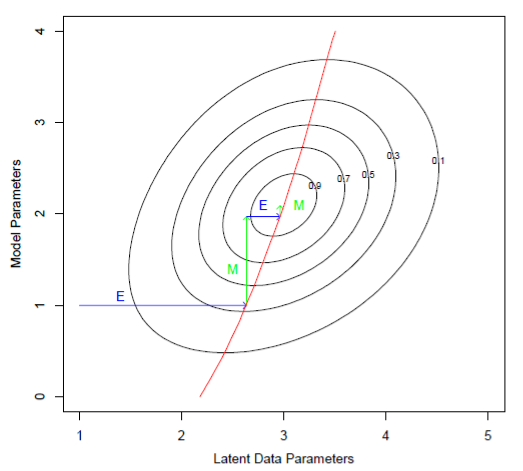
\includegraphics[width=.5\textwidth]{./chap/1chap/6sec/images/3_emAlgo.PNG}
	\end{center}
	\caption{The contours of the (augmented) observed data log-likelihood $F(\theta,\tilde{P})$
	The $E$ step is equivalent to maximizing the log-likelihood over the parameters of the 
	latent data distribution. The $M$ step maximizes it over the parameters of the 
	log-likelihood. The red curve corresponds to the observed data log-likelihood a profile
	obtained by maximizing $F(\theta', \tilde{P})$ for each value of $\theta'$}
	\label{fig:3_emAlgo}
\end{figure}
\subparagraph{Gibbs Sampler}
\begin{enumerate}
	\item Take some initial values $U_{k}^{(0)}$ for $k\in\inter{1}{K}$
	\item Repeat for $t\in\inter{1}{?}$:
		For $k\in\inter{1}{K}$ generate $U_{k}^{(t)}$ from 
		$$ \Pr(U_{k}^{(t)}|U_{1}^{(t)}, \cdots U_{k-1}^{(t)}, U_{k+1}^{(t-1)},\cdots U_{K}^{(t-1)})$$
	\item Continue step 2 until the joint distribution of $\left( U_{j}^{(t)} \right)_{1\leq j\leq K}$
\end{enumerate}
\paragraph{MCMC (Markov chain Monte Carlo) for Sampling from the Posterior}
Gibbs sampling  is an MCMC procedure that is closely related to the EM Algorithm: the main 
difference  is that is it samples from the conditional distributions rather than maximizing over 
them. \\
More formally, Gibbs sampling produces a Markov chain whose stationary distribution is the 
true joint distribution, and hence the term of ``Markov Chain Monte Carlo''
\subparagraph{Gibbs sampling for mixtures}
\begin{enumerate}
	\item Take some initial values: $\theta^{(0)}=(\mu_{1}^{(0)}, \mu_{2}^{(0)})$
	\item Repeat for $t\in\inter{1}{?}$:
		\begin{enumerate}[label=(\alph*)]
			\item For $i\in\inter{1}{N}$ generate $\bm{\Delta}_{i}^{(t)}\in\left\{0,1
				\right\}$ with $\Prob{\bm{\Delta}_{i}^{(t)}=1}=\hat{\gamma}_{i}(
				\theta^{(t)})$
			\item Set
				\begin{align*}
					\hat{\mu}_{1} = & \dfrac{\su{{i=1}}{N}\left(1-\bm{\Delta}_{i}^{(t)}\right)y_{i}}{\su{{i=1}}{N}\left(1-\bm{\Delta}_{i}^{(t)}\right)}\\
					\hat{\mu}_{2} = & \dfrac{\su{{i=1}}{N}\bm{\Delta}_{i}^{(t)}y_{i}}{\su{{i=1}}{N}\bm{\Delta}_{i}^{(t)}}
				\end{align*}
					and generate $\mu_{1}^{(t)}\hookrightarrow\mathcal{N}(\hat{\mu}_{1}, \hat{\sigma}_{1}^{2})$ and $\mu_{1}^{(t)}\hookrightarrow\mathcal{N}(\hat{\mu}_{2},
					\hat{\sigma}_{2}^{2})$
			\item Continue until the joint distribution of $\left(\Delta^{(t)},\mu_{1}^{(t)}, \mu_{2}^{(t)}\right)$ does not change.
		\end{enumerate}
\end{enumerate}

\paragraph{Bagging}
We show how to use the bootstrap to improve the estimate or prediction itself.\\
For each bootstrap $\bm{Z}^{*b}$ for $b\in\inter{1}{B}$ we fit our model, giving prediction
$\hat{f}^{*b}(x)$. The bagging estimate is defined by:
$$ \hat{f}_{bag}(x) = \dfrac{1}{B}\su{{b=1}}{B}\hat{f}^{*b}(x)$$
It is a Monte Carlo estimate of the true bagging estimate, approaching it as $B\rightarrow \infty$.o
Suppose $\xi$
\paragraph{Model Averaging and Stacking}
The posterior distribution of $\xi$ is
$$ \ProbC{\bm{Z}}{\xi} = \su{{m=1}}{M}\ProbC{M_{m},\bm{Z}}{\xi}\ProbC{\bm{Z}}{M_{m}}$$
with posterior $\E{\xi|\bm{Z}} = \su{{m=1}}{M}\E{\xi|M_{m},\bm{Z}}\ProbC{\bm{Z}}{M_{m}}$.
This Bayesian prediction is a weighted average of the individual predictions with weights 
proportional to the posterior probability of each model. This formulation leads to a number
of different model-averaging strategies.

\paragraph{Stochastic Search: Bumping}
\emph{Bumping} uses bootstrap sampling to move randomly through model space. 
In detail we draw bootstrap samples $\left(\bm{Z}^{*j}\right)_{1\leq j\leq B}$ and fit our model
to each giving predictions $\hat{f}^{*b}(x), b\in\inter{1}{B}$. We then choose the model that 
produces the smallest prediction error, averaged over the \emph{original training set}.
$$ \hat{b}=\min\limits_{b}\su{{i=1}}{N}\left[y_{i}-\hat{f}^{*b}(x_{i})\right]^{2}$$

%\subsection{lab: Non-linear modeling}
%\begin{itemize}
 \item
 \end{itemize}

%\subsection{Exercises}
%\begin{itemize}
 \item
 \end{itemize}


\section{Tree-based-methods}
\begin{itemize}
	\item
 \end{itemize}
\subsection{The basics of decision trees}
\begin{itemize}
	\item
 \end{itemize}

\subsection{Bagging, RandomForest and Boosting}
\paragraph{Bagging}
\subparagraph{Bootstrap aggregation (bagging) definition}
It is a \tB{general-purpose procedure for reducing the variance of a
statistical learning method}; we introduce it here because it is
particularly useful and frequently used in the context of decision
trees.\\
In other words for estimating $\hat{f}(x)$, the prediction at input x, we could calculate $\left(f^{i
}(x)\right)_{1\leq i\leq B}$ using $B$ separate training sets, and average them in order to
obtain a single low-variance statistical learning model.\\
We then \sB{train our method on the $b^{th}$ bootstrapped training set in
order to get $\hat{f}^{*b}(x)$}, and finally average all the predictions
to obtain:
\begin{center}
	\encB{$\hat{f}_{bag}(x)=\dfrac{1}{B}\su{{b=1}}{B}\hat{f}^{*b}(x)$}
\end{center}
This is called bagging.

\emph{Python Code}
\begin{python}
import pandas as pd
import sklearn
from sklearn import tree
from sklearn.ensemble import BaggingClassifier,
    BaggingRegressor

y, X = df.iloc[:, 0], df.iloc[:, 1:]
bagging = BaggingClassifier(tree.DecisionTreeClassifier(),
    max_samples=0.5, max_features=0.5)
\end{python}

\subparagraph{Out-of-Bag Error Estimation}
The key to bagging is that trees are repeatedly fit to bootstrapped subsets of the observations.

\paragraph{Random Forest}
When building these decision trees, \sR{each time a split in a tree is 
considered, a random sample of $m$ predictors is chosen as split 
candidates from the full set of $p$ predictors}.\\
In building a random forest, at each split in the tree the algorithm
is \emph{not even allowed to consider} a majority of the available
predictors.

\subparagraph{Random Forest for Regression or Classification}
\begin{enumerate}
	\item For $b\in\inter{1}{B}$
		\begin{enumerate}[label=(\alph*)]
			\item \sB{Draw a bootstrap sample $\bm{Z}^{*}$ of size $N$} from the training
				data
			\item \sB{Grow a random-forest tree $T_{b}$ to the bootstrapped data}, by
				recursively repeating the following steps for each terminal mode
				of the tree, until the minimum node size $n_{min}$ is reached.
				\begin{enumerate}[label=\alph*]
					\item[i.] Select $m$ variables at random from the $p$ 
						variables
					\item[ii.] Pick the best variable/split-point among the $m$
					\item[iii.] Split the node into 2 daughter nodes.
				\end{enumerate}
		\end{enumerate}
	\item Output the ensemble of trees $\left\{T_{b}\right\}_{1}^{B}$
\end{enumerate}
\textit{Regression}: \enc{$\hat{f}_{rf}^{B}(x) = \dfrac{1}{B}\su{{b=1}}{B}T_{b}(x)$}\\
\textit{Classification}: Let $\hat{C}_{b}(x)$ be the class prediction of the $b^{th}$ 
random-forest tree, then $\hat{C}_{rf}^{B}(x)=majority\_vote\left\{\hat{C}_{b}(x)\right\}_{1}^{B}$

\subparagraph{Python Code}
\begin{python}
import pandas as pd
import sklearn
from sklearn.ensemble import RandomForestClassifier,
    RandomForestRegressor

y, X = df.iloc[:, 0], df.iloc[:, 1:]
clf = RandomForestClassifier(n_estimator=10)
\end{python}

\paragraph{Boosting}
\subparagraph{Boosting for Regression Trees}
The motivation for boosting was a procedure that combines the outputs of many ``weak'' classifiers
to produce a powerful ``committee'''. A \sB{weak classifier is one whose error rate is only slightly
better than random guessing}.
\begin{enumerate}
	\item Set $\hat{f}(x)=0$ and $r_{i}=y_{i}$ for all $i$ in the
		training set.
	\item For $b\in\inter{1}{B}$ repeat:
		\begin{enumerate}[label=\alph*]
			\item Fit a tree $\hat{f}^{b}$ with $d$ splits
				($d+1$ terminal nodes) to the training
				data (X,r)
			\item Update $\hat{f}$ by adding in a shrunken
				version of the new tree:
				$$
				\hat{f}(x)\leftarrow \hat{f}(x)+\lambda
				\hat{f}^{b}(x)
				$$
			\item Update the residuals,
				$r_{i}\leftarrow r_{i}-\lambda \hat{f}^{b}(x_{i})$
			\end{enumerate}
	\item Output the boosted model, $\hat{f}(x)=\su{{b=1}}{B}\lambda\hat{f}^{b}(x)$
\end{enumerate}

\subparagraph{Boosting methods}
Consider a two-class problem, with the output variable coded as $Y\in\left\{-1,1\right\}$. Given a
vector of predictor variables $X$, a classifier $G(X)$ produces a prediction taking one of the 
2 values $\{-1,1\}$
\begin{figure}[H]
	\begin{center}
		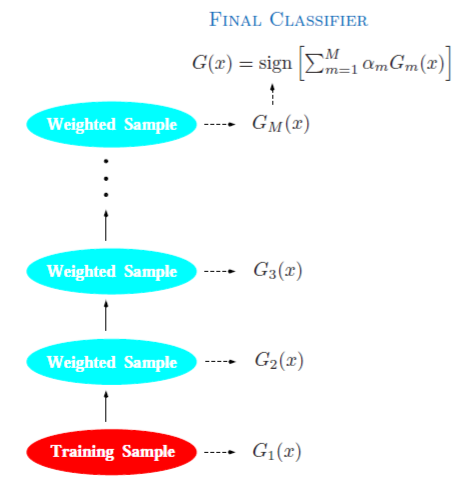
\includegraphics[width=.5\textwidth]{./chap/1chap/7sec/images/1_adaboost.PNG}
	\end{center}
	\caption{Schematic of AdaBoost. Classifiers are trained on weighted versions of the 
	dataset, and then combined to produce a final prediction.}
	\label{fig:1_adaboost}
\end{figure}
\begin{center}
	\encB{$ G(x) = sign\left( \su{{m=1}}{M}\alpha_{m}G_{m}(x) \right)$}
\end{center}
Here \sB{$\alpha_{m}$'s are computed by the boosting algorithm and weight the contribution of each 
respective $G_{m}(x)$}. Their effect is to give higher influence to the more accurate classifiers in
the sequence.

\subparagraph{AdaBoost.M1}
\begin{enumerate}
	\item Initialize the observation weights $w_{i}=\frac{1}{N}, i\in\inter{1}{N}$
	\item For $m\in\inter{1}{M}$:
		\begin{enumerate}[label=\alph*]
			\item Fit a classifier $G_{m}(x)$ to the training data using weights $w_{i}$
			\item Compute:
				$$ err_{m} = \dfrac{\su{{i=1}}{N}\omega_{i}I\left(y_{i}\neq G_{m}(x_{i})\right)}{\su{{i=1}}{N}\omega_{i}}$$
			\item Compute \tV{$\alpha_{m}=\log\left(\dfrac{1-err_{m}}{err_{m}}\right)$}
			\item Set \tV{$\omega_{i} \leftarrow \omega_{i}e^{\alpha_{m}I(y_{i}\neq G_{m}(x_{i}))}$ for $i\in\inter{1}{N}$}
		\end{enumerate}
	\item Output $G(x)=sign\left[\su{{m=1}}{M}\alpha_{m}G_{m}(x)\right]$
\end{enumerate}
\subparagraph{Python Code}
\begin{python}
import pandas as pd
import sklearn
from sklearn.ensemble import AdaBoostClassifier,
    AdaboostRegressor
from sklearn.model_selection import corss_val_score

y, X = df.iloc[:, 0], df.iloc[:, 1:]
clf = AdaBoostClassifier(n_estimator=100)
scores = corss_val_score(clf, X, y, cv=5)
\end{python}

\paragraph{Boosting Fits an Additive Model}
\begin{center}
\encB{$ f(x)=\su{{m=1}}{M}\beta_{m}b(x;\gamma_{m})$}
\end{center}
where $\beta_{m}$'s are the expansion coefficients and $b(x;\gamma)\in\mathbb{R}$ are usually
simple functions of the multivariate argument $x$, characterized by a set of parameters $\gamma$
\subparagraph{Forward Stagewise Additive Modeling}
\begin{enumerate}
	\item Initialize $f_{0}(x)=0$
	\item For $m\in\inter{1}{M}$
		\begin{enumerate}[label=\alph*]
			\item Compute \tV{$(\beta_{m},\gamma_{m}) = \min\limits_{\beta,\gamma}\su{{i=1}}{N}L(y_{i},f_{m-1}(x_{i})+\beta b(x_{i};\gamma))$}
			\item Set $f_{m}(x)=f_{m-1}(x)+\beta_{m}b(x;\gamma_{m})$
		\end{enumerate}
\end{enumerate}

\paragraph{Forward Stagewise Additive Modeling}
\sB{At each iteration $m$, one solves the optimal basis function $b(x;\gamma_{m})$ and corresponding
coefficient $\beta_{m}$ to add the current expansion $f_{m-1}(x)$.} This procedure $f_{m}(x)$,
and the process is repeated.
For the squared-error loss: $L(y,f(x))=\left(y-f(x)\right)^{2}$ one has 
\begin{align*}
L(y_{i},f_{m-1}(x_{i})+\beta b(x_{i};\gamma)) =& \left(y_{i}-f_{m-1}(x)-\beta 
b(x_{i};\gamma)\right)\\
=& \left(r_{im}-\beta b(x_{i},\gamma)\right)^{2}
\end{align*}
where $r_{im}=y_{i}-f_{m-1}(x_{i})$ is simply the residual of the current model on the $i^{th}$
observation.

\paragraph{Loss Functions and Robustness}
\subparagraph{Robust Loss Functions for Classification}
The minimizer of the corresponding risk on the population is :
$$ f^{*}(x)=\min\limits_{f(x)}\mathbb{E}_{Y|x}\left(Y-f(x)\right)^{2} = \E{Y|X}=2\ProbC{x}{Y=1}
-1$$
\begin{figure}[H]
	\begin{center}
		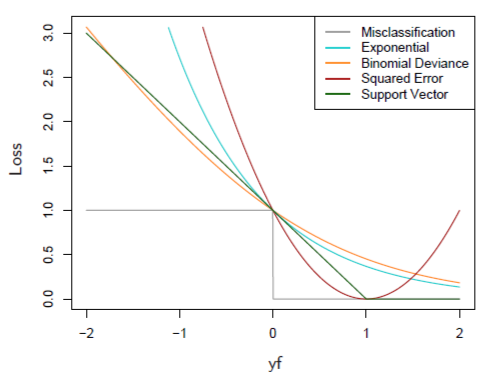
\includegraphics[width=.6\textwidth]{./chap/1chap/7sec/images/2_LossFunction.PNG}
	\end{center}
	\caption{The response is $y=\pm 1$ the prediction is $f$, with class prediction $sign(f)$.
	The losses are misclassification: $I(sign(f)\neq y)$; exponential: $exp(-yf)$; binomial
	deviance $\log(1+e^{-2yf})$; squared error $(y-f)^{2}$; and support vector: $(1-yf)_{+}$}
	\label{fig:2_LossFunction}
\end{figure}
\subparagraph{Python Code}
\begin{python}
import pandas as pd
import sklearn
from sklearn.ensemble import GradientBoostingClassifier
from sklearn.model_selection import train_test_split

y, X = df.iloc[:, 0], df.iloc[:, 1:]
X_train, X_test, y_train, y_test = train_test_split(
    X, y, random_state=0)
clf = GradientBoostingClassifier(
   loss = 'deviance', # {'deviance', 'exponential'}
   random_state = 0
)
print(clf.score(X_test, y_test))
\end{python}
\subparagraph{Robust Loss Functions for Regression}
One such criterion is the Huber loss criterion used for M-regression
$$ L(y,f(x))=
\begin{cases}
	\left(y-f(x)\right)^{2} \Leftarrow |y-f(x)|\leq \delta \\
	2\delta|y-f(x)|-\delta^{2} \Leftarrow |y-f(x)|> \delta
\end{cases}
$$
\begin{figure}[H]
	\begin{center}
		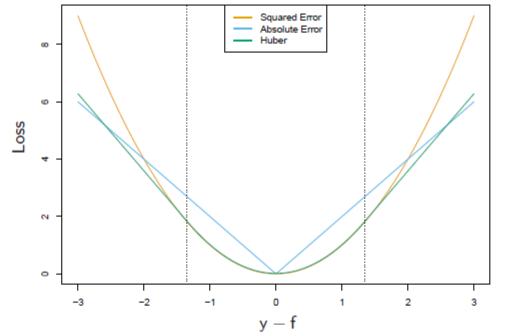
\includegraphics[width=.7\textwidth]{./chap/1chap/7sec/images/3_LossFunction_reg.PNG}
	\end{center}
	\caption{The Huber loss function combines the good properties of squared-error loss near
	zero and absolute error loss when $|y-f|$ is large}
	\label{fig:3_LossFunction_reg}
\end{figure}

\subparagraph{Python Code}
\begin{python}
import pandas as pd
import sklearn
from sklearn.ensemble import GradientBoostingRegressor
from sklearn.model_selection import train_test_split

y, X = df.iloc[:, 0], df.iloc[:, 1:]
X_train, X_test, y_train, y_test = train_test_split(
    X, y, random_state=0)
reg = GradientBoostingRegressor(
   loss = 'huber', # {'ls', 'lad', 'huber'}
   random_state = 0
)
print(reg.score(X_test, y_test))
\end{python}



\paragraph{Procedures for Data Mining}
\begin{figure}[H]
	\begin{center}
		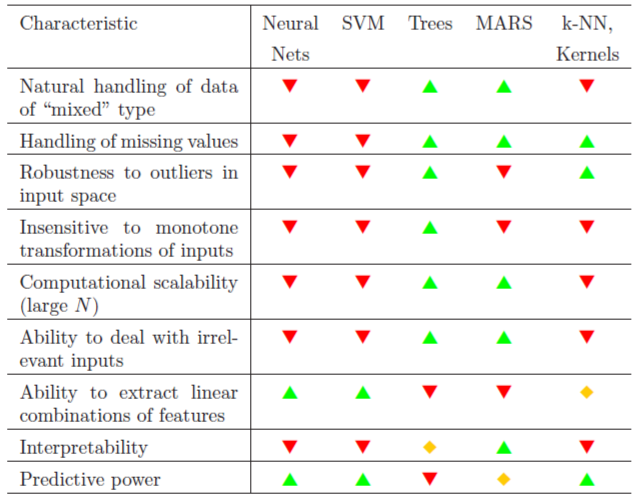
\includegraphics[width=\textwidth]{./chap/1chap/7sec/images/4_compMeth.PNG}
	\end{center}
	\caption{Some characteristics of different learning methods.Green=good, Yellow=fair, 
	Red=poor}
	\label{fig:4_compMeth}
\end{figure}

\paragraph{Boosting Trees}
Regression and classification trees partition the space of all joint predictor variable values
into disjoint regions $R_{j},j\in\inter{1}{J}$ as represented by the terminal nodes of the tree.\\
A constant $\gamma_{j}$ is assigned to each such region and the predictive rule is :
$x\in R_{j} \Rightarrow f(x)=\gamma_{j}$. Thus a tree can be formally expressed as:
$$ T(x;\Theta)=\su{{j=1}}{J}\gamma_{j}I(x\in R_{J})$$
with parameters $\Theta=\left\{R_{j},\gamma_{j}\right\}_{1}^{J}$
The parameters are found by minimizing the empirical risk: 
$\Theta = \min\limits_{\Theta}\su{{j=1}}{J}\su{{x_{i}\in R_{j}}}{}L(y_{i},\gamma_{j})$

\paragraph{Numerical Optimization via Gradient Boosting}
The goal is to minimize $L(f)=\su{{i=1}}{N}L(y_{i},f(x_{i}))$ with respect to $f$, where here
$f(x)$ is constrained to be a sum of trees. Ignoring this constraint, minimizing $L(f)$ can be
viewed as a numerical optimization:
$$ \hat{\bm{f}} = \min\limits_{f}L(\bm{f})$$ where the parameters $\bm{f}\in\mathbb{R}^{N}$ are
the values of the approximating function $f(x_{i})$ such as $\bm{f} = \left(f(x_{i})
\right)_{1\leq i\leq N}^{T}$
Numerical optimization procedures solves the previous equation as a sum of component vectors:
$$ \bm{f}_{M} = \su{{m=0}}{M}\bm{h}_{m}, \bm{h}_{m}\in\mathbb{R}^{N}$$

\subparagraph{Steepest Descent}
Steepest descent chooses \tB{$\bm{h}_{m} = -\rho_{m}\bm{g}_{m}, (\rho_{m}, \bm{g}_{m})\in\mathbb{R}
\times\mathbb{R}^{N}$, $\bm{g}_{m}$ is the gradient of $L(\bm{f})$ evaluated at $\bm{f}=\bm{f}_{
m-1}$}. The components of the gradient $\bm{g}_{m}$ are: 
\begin{center}
\encB{$ g_{im} = \left[\dfrac{\partial L(y_{i},f(x_{i}))}{\partial f(x_{i})}\right]_{f(x_{i}=f_{m-1}(
x_{1}))}$} 
\end{center}
The step length $\rho_{m}$ is the solution to 
$ \rho_{m}=\min\limits_{\rho}L\left(\bm{f}_{m-1}-\rho\bm{g}_{m}\right)$, the current solution
is then updated 
\begin{center}
	\enc{$ \bm{f}_{m} = \bm{f}_{m-1} -\rho_{m}\bm{g}_{m}$}
\end{center}

\begin{figure}[H]
	\begin{center}
		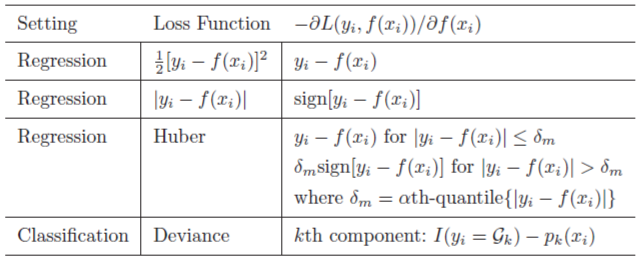
\includegraphics[width=\textwidth]{./chap/1chap/7sec/images/5_common_gradients.PNG}
	\end{center}
	\caption{Gradients for commonly used loss functions}
	\label{fig:5_common_gradients}
\end{figure}

Gradient Tree Boosting Algorithm
\begin{enumerate}
	\item Initialize $f_{0}(x)=\min\limits_{\gamma}\su{{i=1}}{N}L(y_{i},\gamma)$
	\item For $m\in\inter{1}{M}$:
		\begin{enumerate}[label=(\alph*)]
			\item For $i\in\inter{1}{N}$ compute: $r_{im}=-\left[\dfrac{\partial L(y_{i},f(x_{i}))}{\partial f(x_{i})}\right]_{f=f_{m-1}}$
			\item  Fit a regression tree to the targets $r_{im}$ giving terminal 
				regions $R_{jm},j\in\inter{1}{J_{m}}$
			\item For $j\in\inter{1}{J_{m}}$ compute: $\gamma_{jm}=\min\limits_{
				\gamma}\su{{x_{i}}\in R_{jm}}{}L(y_{i},f_{m-1}(x_{i}) + \gamma)$
			\item Update $f_{m}(x)=f_{m-1}(x)+\su{{j=1}}{J_{m}}\gamma_{jm}I(x\in\mathbb{R}_{jm})$
		\end{enumerate}
	\item Output $\hat{f}(x)=f_{M}(x)$
\end{enumerate}


\subsection{Lab: decision trees}
\begin{itemize}
 \item
 \end{itemize}

\subsection{Exercises}
\begin{itemize}
 \item
 \end{itemize}


\section{Support vector machines}
\subsection{Maximal margin classifier}
\begin{itemize}
	\item
 \end{itemize}

\subsection{Support vectors classifiers}
\paragraph{Aim}
Considering that the maximal margin hyperplane is extremely sensitive
to a change in a single observation, it may have overfit the training
data.\\
In this case we might be willing to consider a classifier based on a
hyperplane that does not perfectly separate the 2 classes therewith to
get 
\begin{itemize}
	\item \tB{Greater robustness} to individual observation
	\item \tB{Better classification} of most of the training observations
\end{itemize}
And the \emph{Support Vector Classifier} does exactly this.

\paragraph{Details}
The support vector classifier classifies a test observation depending
on which side of the hyperplane it lies.
\begin{figure}[H]
	\begin{center}
		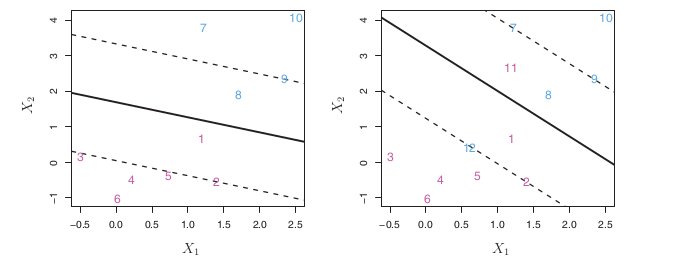
\includegraphics[width=\textwidth]{./chap/1chap/8sec/images/2supportVectorClassifier.png}
	\end{center}
	\caption{Left:Purple observations: 3, 4, 5 and 6 are on the 
	correct side, 2 is on the margin and 1 is on the wrong side.\\
	Blue observations: 7 and 10 are on the correct side, 9 on the
	margin and 8 on the wrong side\\
	Right: same as left panel with two additional points, 11 and 12
	which are on the wrong side}
	\label{fig:8.1 supportVectorClassifier}
\end{figure}

It is the solution to the optimization problem
\begin{center}
\enc{$
\max\limits_{\prtH{\beta}{i}{0}{p}\prtH{\epsilon}{i}{1}{n},M}~M~
\text{ subject to }
\begin{cases}
	\su{{j=1}}{p}\beta_{j}^{2}=1\\
	y_{i}\left( \beta_{0}+\su{{j=1}}{p}\beta_{j}x_{ij} \right) >
	M(1-\epsilon_{i})\\
	\epsilon_{i}\geq 0, \su{{i=1}}{n}\epsilon_{i}\leq C
\end{cases}$}
\end{center}
where $C$ is a nonnegative tuning parameter, $M$ is the width of the 
margin.\\
$\prth{\epsilon}{i}{n}$ are \emph{slack variables} that allow 
individual observations to be on the wrong side of the margin or the
hyperplane.
We have:
$$
\begin{cases}
	\tB{\epsilon_{i}=0}\Rightarrow i^{th}\text{ observation is on the
	\sB{correct side of the margin}}\\
	\tB{\epsilon_{i}>0}\Rightarrow i^{th}\text{ observation is on the
	\sB{wrong side of the margin}}\\
	\tB{\epsilon_{i}>1}\Rightarrow i^{th}\text{ observation is on the
	\sB{wrong side of the hyperplane}}\\
\end{cases}
$$
$C$ determines the number and severity of the violations to the margin
that we will tolerate.\\

In practice $C$ is treated as a tuning parameter that is generally 
chosen via cross-validation.\\

It turns out an observation that only observations that lies strictly
on the correct side of the margin does not affect the support vector
classifier.

\subsection{Support vectors machines}
\paragraph{Classification with non-linear decision boundaries}
Rather than fitting a support vector classifier using $p$ features
we could instead fit a support vector classifier using $2p$ features,
then we get for $\left(X_{i},X_{i}^{2}\right)_{0\leq i\leq p}$:
$$
\max\limits_{\left(\beta_{i1}\right)_{0\leq i\leq p}\left(\beta_{i2}\right)_{1\leq i\leq p}\prtH{\epsilon}{i}{1}{n},M} M\\
\text{ subject to }
\begin{cases}
	\su{{j=1}}{p}\su{{k=1}}{2}\beta_{jk}^{2}=1\\
	y_{i}\left( \beta_{0}+\su{{j=1}}{p}\beta_{j1}x_{ij}+\su{{j=1}}{p}\beta_{j2}x_{ij}^{2}\right) >
	M(1-\epsilon_{i})\\
	\epsilon_{i}\geq 0, \su{{i=1}}{n}\epsilon_{i}\leq C
\end{cases}
$$

\paragraph{Support Vector Machine}
The linear \tB{support vector classifier} can be represented as :
\begin{center}
\enc{$
f(x)=\beta_{0} + \su{{i\in\mathcal{S}}}{}\alpha_{i}\sP{x_{i}}{x_{i'}}$}
\end{center}
where $\prth{\alpha}{i}{n}$ are parameters.\\
It turns out that $\alpha_{i}$ is nonzero only for the support vectors
in the solution. So \sB{$\mathcal{S}$ is the collection of indices of 
support vectors in the solution}.\\

We replace inner product with a generalization of the inner product
of the form:
$K(x_{i},x_{i'})$
Where $K$ is some function that we will refer to as a \emph{kernel}.
A kernel is a function that quantifies the similarity of 2 observations

\subparagraph{Linear Kernel}
$K(x_{i},x_{i'})=\tB{\su{{j=1}}{p}x_{ij}x_{i'j}}$ essentially \sB{quantifies
the similarity of a pair of observations} using Pearson (standard)
correlation.
\subparagraph{Polynomial Kernel}
$K(x_{i},x_{i'})=\tB{\left( 1 + \su{{j=1}}{p}x_{ij}x_{i'j} \right)^{d}}$
instead of the standard linear kernel in the support vector classifier
algorithm leads to a \sB{much more flexible decision boundary}.
\subparagraph{Radial Kernel}
$K(x_{i},x_{i'})=\tB{\exp\left( -\gamma\su{{j=1}}{p}(x_{ij}x_{i'j})^{2} \right)}$
with $\gamma\geq 0$, the radial kernel has \sB{very local behavior}, in the
sens that only nearby training observations have an effect on the class
label of a test observation.
\begin{figure}[H]
	\begin{center}
		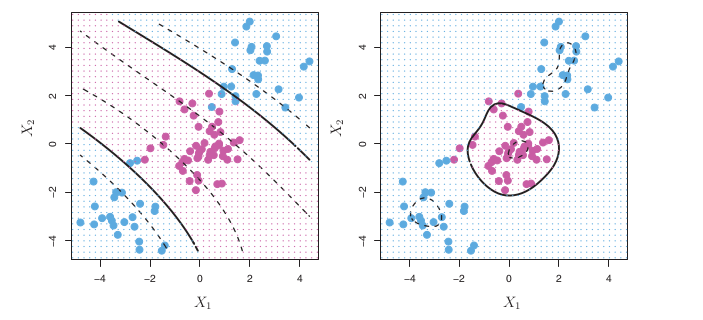
\includegraphics[width=\textwidth]{./chap/1chap/8sec/images/3polynomialRadialKernel.png}
	\end{center}
	\caption{Left: a SVM with a polynomial kernel of degree 3 is
	applied to non-linear data.\\
	Right: a SVM  with a radial kernel is applied.}
	\label{fig:8.3polynomialRadialKernel}
\end{figure}

\subparagraph{Python Code}
\begin{python}
import pandas as pd
import sklearn
from sklearn import tree
from sklearn import svm

y, X = df.iloc[:, 0], df.iloc[:, 1:]
clf = svm.SVC(
   C = 1.0, # Regularization parameter
   kernel = 'linear', # {'linear', 'poly', 'rbf'}
)
clf.fit(X, y)

\end{python}

\subsection{SVMs with more than 2 classes}
\paragraph{One-Versus-One Classification}
Suppose that we would like to perform classification using SVMs, and
there are $K>2$ classes.\\
We classify a test observation using each of the $\binom{K}{2}$ 
classifier and we tally the number of times that the test observation
is assigned to each of the $K$ classes. The final classification is 
performed by assigning the test observation to the class to which it
was most frequently assigned in these $\binom{K}{2}$ pairwise
classifications.

\paragraph{One-Versus-All Classification}
We fit $K$ SVMs, each time comparing one of the $K$ classes to the 
remaining $K-1$ classes.

\subsection{Relationship to Ridge Regression}
It turns out that one can \sB{rewrite solution for fitting the support}
vector classifier $f(X)=\beta_{0}+\su{{i=1}}{p}\beta_{i}X_{i}$
\begin{center}
\encB{$
\min\limits_{\prtH{\beta}{i}{1}{p}}\left\{ \su{{i=1}}{n}max[0,~~1-y_{i}f(x_{i})]+\lambda\su{{j=1}}{p}\beta_{j}^{2} \right\}
$}
\end{center}
where $\lambda$ is a nonnegative tuning parameter, and 
$P(\beta)=\su{{j=1}}{p}\beta_{j}^{2}$ (ridge regression) and 
$P(\beta)=\su{{j=1}}{p}|\beta_{j}|$ (lasso)
Recall that the ``Loss + Penality'' form is:
$\min\limits_{\prtH{\beta}{i}{1}{p}}{L(X,y,\beta)+\lambda P(\beta)}$\\
For the ridge regression and the lasso both loss functions take this
form with:\\
$L(X,y,\beta)=\su{{i=1}}{n}\left( y_{i}-\beta_{0}-\su{{j=1}}{p}x_{ij}\beta_{j} \right)^{2}$\\
For the SVM the loss function istead takes the form:\\
$L(X,y,\beta)=\su{{i=1}}{n}max[0,~~1-y_{i}\left( \beta_{0}+\su{{j=1}}{p}\beta_{j}x_{ij} \right)]$

\paragraph{Regression and Kernels}
\sB{Suppose we consider approximation of the regression function in terms of a set of basis 
functions} $\left\{h_{m}(x)|m\in\inter{1}{M}\right\}$: $f(x)=\su{{m=1}}{M}\beta_{m}h_{m}(x)+
\beta_{0}$ To estimate $\beta$ and $\beta_{0}$ we minimize:
$$ H(\beta,\beta_{0})=\su{{i=1}}{N}V(y_{i}-f(x_{i}))+\dfrac{\lambda}{2}\su{}{}\beta_{m}^{2}$$
for some general error measure $V(r)$.\\
\sB{For any choice of $V(r)$}, the solution $\hat{f}(x)=
\su{}{}\hat{\beta}_{m}h_{m}(x)+\hat{\beta}_{0}$ has the form : 
\begin{center}
	\encB{$ \hat{f}(x)=\su{{i=1}}{N}\hat{\alpha}_{i}K(x,x_{i})$}
\end{center}
with $K(x,y)=\su{{m=1}}{M}h_{m}(x)h_{m}(
y)$\\
We estimate $\beta$ by minimizing the penalized least squares criterion:
$$ H(\beta)=\left(\bm{y}-\bm{H}\beta\right)^{T}\left(\bm{y}-\bm{H}\beta\right) + 
\lambda\norm{\beta}^{2}$$
The solution is $\hat{\bm{y}} = \bm{H}\hat{\beta}$ with $\hat{\beta}$ determined by:
$-\bm{H}^{T}(\bm{y}-\bm{H}\hat{\beta}) + \lambda\hat{\beta} = 0$
We can pre-multiply by $\bm{H}$ to give: 
$$ \bm{H}\hat{\beta} = \left(\bm{H}\bm{H}^{T}+\lambda\bm{I}\right)^{-1}\bm{H}\bm{H}^{T}\bm{y}$$


\subparagraph{Python Code}
\begin{python}
import pandas as pd
import sklearn
from sklearn.kernel_ridge import KernelRidge

y, X = df.iloc[:, 0], df.iloc[:, 1:]
clf = KernelRidge(
    alpha=0.5,
    kernel='linear')
clf.fit(X, y)
\end{python}

\subsection{Linear Discriminant Analysis}
There is a class of techniques that produce better classifiers than LDA by directly generalizing
LDA.

\paragraph{Flexible Discriminant Analysis}
This is a method for performing LDA using linear regression on derived responses.\\
We assume that we have observations with a quantitative response $G$ falling into one $K$ classes
$\mathcal{G}=\left\{k\right\}_{1\leq k\leq K}$ each having measured features $X$.\\
Suppose $\theta:\mathcal{G}\mapsto\mathbb{R}$ is a function that assigns scores to the classes,
such that the transformed class labels are optimally predicted by linear regression on $X$: If
our training has the form $\left(g,x_{i}\right)$ for $i\in\inter{1}{N}$ we solve:
$$ \min\limits_{\beta,\theta}\su{{i=1}}{N}\left(\theta(g_{i})-x_{i}^{T}\beta\right)^{2}$$
with restriction to $\theta$ to avoid a trivial solution (mean zero and unit variance over the 
training data).\\
More generally, we can find up to $L\leq K-1$ sets of independent scorings for the class labels
$\prth{theta}{l}{L}$ and $L$ corresponding linear maps $\eta_{l}(X)=X^{T}\beta_{l}$ with$l\in
\inter{1}{L}$ chosen to be optimal for multiple regression in $\mathbb{R}^{p}$. The scores
$\theta_{l}(g)$ and the maps $\beta_{l}$ are chosen to minimize the averages squared residual:

$$ASR = \dfrac{1}{N}\su{{l=1}}{L}\left[\su{{i=1}}{N}\left(\theta_{l}(g_{i})-x_{i}^{T}\beta_{l}
\right)^{2}\right] $$
Moreover, the Mahalanobis distance of a test point $x$ to the $k^{th}$ class centroid $\hat{\mu}_{
k}$ is given by:
$$ \delta_{J}(x,\hat{\mu}_{k}) = \su{{l=1}}{K-1}\omega_{l}\left(\hat{eta}_{l}(x)-\overline{\eta}_{
l}^{k}\right)^{2} + D(x)$$
where $\overline{\eta}_{l}^{k}$ is the mean of the $\hat{\eta}_{l}(x_{i})$ in the $k^{th}$ class,
and $D(x)$ does not depend on $k$. Here $\omega_{l}$ are coordinate weights that are defined
in terms of the mean squared residual $r_{l}^{2}$ of the $l^{th}$ optimally scored fit:
$$ \omega_{l}= \dfrac{1}{r_{l}^{2}(1-r_{l}^{2})}$$ To summarize LDA can be performed by a
sequence of linear regressions, followed by classification to the closest class centroid in
the space of fits. The analogy applies both to the reduced rank version or the full rank case
when $L=K-1$. \\
The real power of this result is in the generalizations that it invites, we can replace the linear
regression fits $\eta_{l}(x) = x^{T}\beta$ by far more flexible non-parametric fits, and by 
analogy achieve a more flexible classifier than LDA. In this more general form the regression 
problems are defined via the criterion:
$$ ASR\left(\left\{\theta_{l},\eta_{l}\right\}_{l=1}^{L}\right)=\dfrac{1}{N}\su{{l=1}}{L}\left[
\su{{i=1}}{N}\left(\theta_{l}(g_{i})-\eta_{l}(x_{i}) \right)^{2} +\lambda J(\eta_{l})\right]$$
where $J$ is a regularized appropriate for some forms of non-parametric regression, such as 
smoothing splines, additive splines and lower-order ANOVA spline models.

\paragraph{Penalized Discriminant Analysis}
Although FDA is motivated by generalized optimal scoring, it can also be viewed directly as a
form of regularized discriminant analysis. Suppose the regression procedure used in FDA amounts
to a linear regression onto a basis expansion $h(X)$, with a quatrat

The steps in FDA can be viewed as generalized form of LDA which we call penalized discriminant
analysis or PDA:
\begin{itemize}
	\item Enlarge the set of predictors $X$ via basis expansion $h(X)$
	\item Use penalized LDA in the enlarged space, where the penalized Mahalanobis distance
		is given by:
		i$$D(x,\mu)=\left(h(x)-h(\mu)\right)^{T}\left(\Sigma_{W}+\lambda\Omega \right)^{
		-1}\left(h(x)-h(\mu)\right)$$ where $\Sigma_{W}$ is the within-class covariance
		matrix of the derived variables $h(x_{i})$
	\item Decompose the classification subspace using a penalized metric:
		$$ \max u^{T}\su{}{}\beta u\text{ subject to }u^{T}\left(\Sigma_{W}+\lambda\Omega\right)u = 1$$
\end{itemize}


%\subsection{lab: support vector machines}
%\begin{itemize}
 \item
 \end{itemize}

%\subsection{Exercises}
%\begin{itemize}
 \item
 \end{itemize}


\section{Unsupervised learning}
\begin{itemize}
	\item
 \end{itemize}
\subsection{The challenge of unsupervised learning}
Unsupervised learning is often performed as part of an 
\emph{explaratory data analysis}.

\subsection{Principal compoments analysis}
\begin{itemize}
	\item
 \end{itemize}

\subsection{Clustering methods}
\paragraph{$K$-Means Clustering}
It is a method for finding clusters and cluster centers in a set of unlabeled data. 
\subparagraph{Definition}
The principle lays on the thought that a good clustering is one for
which the within cluster variation is as small as possible. The
within-cluster variation for cluster $C_{k}$is a measure $W(C_{k})$:
\begin{center}
\enc{
$
\min\limits_{\prth{C}{i}{K}}\left\{ \su{{k=1}}{K}W(C_{k}) \right\}
$
}
\end{center}
We need to define the within-cluster variation, the most common choice
is:
\begin{center}
\enc{
$
W(C_{k})=\dfrac{1}{|C_{k}|}\su{ {i,i'\in C_{k}}}{}\su{{j=1}}{p}(x_{ij}-x_{i'j})^{2}
$
}
\end{center}
where \tB{$|C_{k}|$ denotes the cardinal of $k^{th}$ cluster}.

\subparagraph{Algorithm K-Means Clustering}

\begin{enumerate}
	\item Randomly assign a number in $\inter{1}{K}$ to each of the
		observations.
	\item Iterate until the cluster assignment stop changing:
		\begin{enumerate}[label=(\alph*)]
			\item For each $K$ clusters, compute the
				cluster \emph{centroid}. The $k^{th}$
				cluster centroid is the vector of 
				the $p$ feature means for the 
				observations in the $k^{th}$ cluster.
			\item Assign each observation to the cluster
				whose centroid is closet.
			\end{enumerate}
\end{enumerate}
\begin{figure}[H]
	\begin{center}
		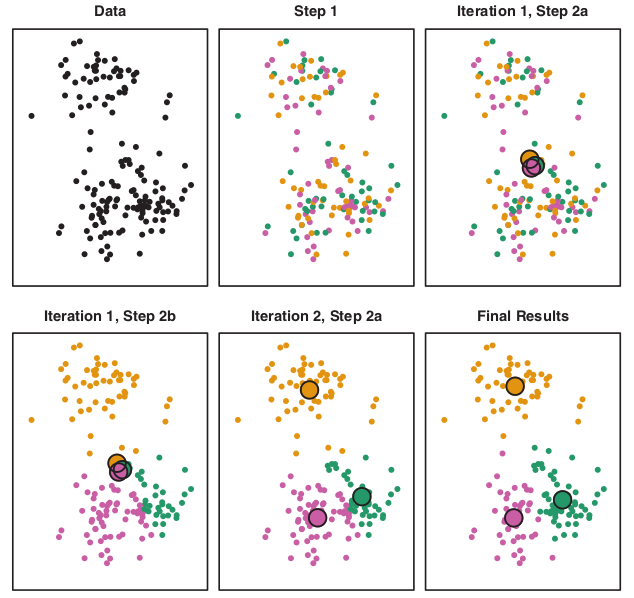
\includegraphics[width=.5\textwidth]{./chap/1chap/9sec/images/1kMeans.png}
	\end{center}
	\caption{Step1: Each observation is randomly assigned\\
	Step(2a): The clusters are computed\\
	Step(2b): Each observation is assigned to the nearest centroid.}
	\label{fig:9.1kMeans}
\end{figure}
\subparagraph{Python Code}
\begin{python}
import pandas as pd
import sklearn
from sklearn.cluster import KMeans

X = df.copy()
kmeans = KMeans(n_clusters=2,
    random_state=0).fit(X)
print(kmeans.labels_)
print(kmeans.cluster_centers_)
\end{python}

\subparagraph{Learning Vector Quantization}
In this technique, prototypes are placed strategically with respect to the decision boundaries
in an ad-hoc way. LVQ is an online algorithm. The idea is that the training points attract
prototypes of the correct class and repel other prototypes.
\begin{enumerate}
	\item Choose $R$ initial prototypes for each class: $\left\{m_{r}(k)|(r,k)\in\inter{1}{R}
		\times\inter{1}{K}\right\}$ by sampling $R$ training points at random from each
		class.
	\item Sample a training point $x_{i}$ randomly (with replacement):
		\begin{enumerate}[label=\alph*]
			\item if $g_{i}=k$ (i.e. they are in the same class), move the prototype
				towards the training point:
				$$ m_{j}(k)\leftarrow m_{j}(k) + \epsilon(x_{i}-m_{j}(k))$$
				where $\epsilon$ is the learning rate
			\item If $g_{i}\neq k$ (i.e, they are in different classes), move the 
				prototype away from the training point:
				$$ m_{j}(k)\leftarrow m_{j}(k) - \epsilon(x_{i}-m_{j}(k))$$
		\end{enumerate}
	\item Repeat step 2, decreasing the learning rate $\epsilon$ with each iteration towards
		zero.
\end{enumerate}

\paragraph{Hierarchical Clustering}
It is an alternative approach which does not require the we commit to
a particular choice of $K$.\\
It results in an attractive tree-based representation of the 
observations, called a \emph{dendrogram}.

\subparagraph{Interpreting a Dendogram}

\begin{figure}[H]
\begin{subfigure}[b]{0.49\textwidth}
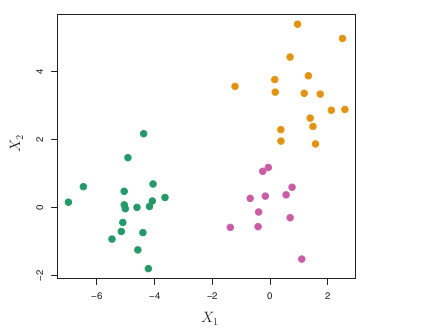
\includegraphics[width=\textwidth]{./chap/1chap/9sec/images/2a_hierarchicalCluster.png}
\caption{Original Data Set}
\label{fig:9.2a_hierarchicalCluster}
\end{subfigure}
\hfill
\begin{subfigure}[b]{0.49\textwidth}
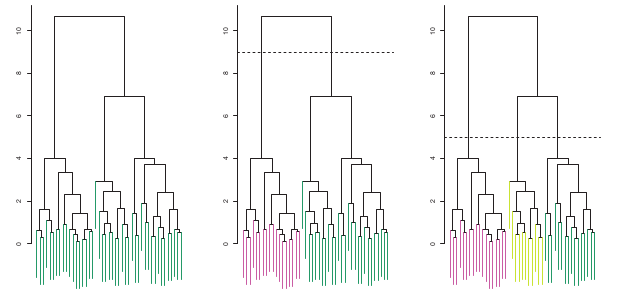
\includegraphics[width=\textwidth]{./chap/1chap/9sec/images/2b_hierarchicalCluster.png}
\caption{Dendrogram}
\label{fig:9.2b_hierarchicalCluster}
\end{subfigure}
\caption{
There are in reality 3 classes, but we will ignore them
and seek to cluster the observations.\\
In the right figure:\\
Left: Dendogram obtained from hierarchically clustering the data of of the left figure.\\
Center: The Dendrogram from the left-hand panel cut at a heigh of 9.
This cut results in 2 distinct clusters.\\
Right: The Dendrogram from the left-hand panel cut at a heigh of 5.
This cut results in 3 distincts clusters.
.}
\end{figure}

\subparagraph{Hierarchical Clustering}
\begin{enumerate}
	\item Begin with $n$ observations and a measure (such as 
		Euclidean distance) of all the $\binom{n}{2}$ pairwise
		dissimilarities.\\ \sB{Treat each observations as its own
		cluster}:
	\item $\forall i\in\inter{2}{n}$:
		\begin{enumerate}
			\item Examine all pairwise inter-cluster 
				dissimilarities among the $i$ cluster
				and \sB{identify the pair of clusters that
				are least dissimilar.\\
				Fuse these 2 cluster}, the dissimilarity
				between these 2 clusters indicates
				the height of the dendrogram at which
				the fusion should be placed.
			\item \sB{Compute the new pairwise inter-cluster
				dissimilarities among the $i-1$
				remaining clusters.}

		\end{enumerate}
\end{enumerate}

\subparagraph{Python Code}
\begin{python}
import pandas as pd
import sklearn
from sklearn.cluster import AgglomerativeClustering

X = df.copy()
clustering = AgglomerativeClustering().fit(X)
print(clustering.labels_)
\end{python}
\paragraph{Adaptive Nearest-Neighbor Methods}
When nearest-neighbor classification is carried out in a high-dimensional feature space, the
nearest neighbors of a point can be very far away, causing bias.\\
To quantify this, consider $N$ data points uniformly distributed in the unit cube $\left[-\dfrac{
1}{2},\dfrac{1}{2}\right]^{p}$. Let $R$ be the radius of a 1-nearest-neighborhood centered at the
origin. Then:
$$ median(R)=v_{p}^{-\frac{1}{p}}\left(1-\dfrac{1}{2}^{\frac{1}{N}}\right)^{\frac{1}{p}}$$ where
$v_{p}r^{^p}$ is the volume of the sphere of radius $r$ in $p$ dimensions.\\

The \emph{Discriminant Adaptive Nearest-Neighbor} (DANN) metric at a query point $x_{0}$ is 
defined by : 
$$ D(x, x_{0}) = (x-x_{0})^{T}\bm{\Sigma}(x-x_{0})$$ where 
\begin{align*}
	\bm{\Sigma} =& \bm{W}^{-\frac{1}{2}}\left[\bm{W}^{-\frac{1}{2}}\bm{B}\bm{W}^{-\frac{1}{2}}
	+\epsilon \bm{I}\right]\bm{W}^{-\frac{1}{2}}\\
	=& \bm{W}^{-\frac{1}{2}}\left[\bm{B}^{*}+\epsilon\bm{I}\right]\bm{W}^{-\frac{1}{2}}
\end{align*}

Here $\bm{W}$ is the pooled within-class covariance matrix $\su{{k=1}}{K}\pi_{k}\bm{W}_{k}$ and
$\bm{W}$ is the between class covariance matrix $\su{{k=1}}{K}\pi_{k}\left(\overline{x}_{k}-
\overline{x}\right)\left(\overline{x}_{k}-\overline{x}\right)$ with $\bm{W}$ and $\bm{B}$
computed using only the $50$ nearest neighbors around $x_{0}$.

\subsection{Lab1: principal compoments analysis}
\begin{itemize}
 \item
 \end{itemize}

\subsection{Lab2: clustering}
\begin{itemize}
 \item
 \end{itemize}

\subsection{Lab3: NCI60 data example}
\begin{itemize}
 \item
 \end{itemize}

\subsection{Exercises}
\begin{itemize}
 \item
 \end{itemize}



\end{document}
